In this chapter, we take an in-depth look at one of the most natural and ``basic'' properties to test, \emph{uniformity}: 
\begin{framed}
Is the unknown distribution \emph{the} uniform distribution $\uniform_\ab$ over the domain $[\ab]$, or does it significantly deviate from being uniform?
\end{framed}
Formally, recalling~\cref{def:testing}, we define uniformity testing by letting $\property_\ab \eqdef \{\uniform_\ab\}$ (a singleton), and $\class_\ab=\distribs{\ab}$. Of course, while the uniform distribution is a rather fundamental one, one might instead have a different reference distribution in mind, \eg a particular Binomial distribution, or a Zipf one, or an arbitrary probability distribution provided as a vector of $\ab$ probabilities. This generalization is known (in the computer science community) as \emph{identity testing}, and also goes by the name of \emph{one-sample goodness-of-fit}. While identity testing might seem to be a strictly more general problem than uniformity testing, the two are closely related. Clearly, identity testing is at least as hard as uniformity testing; but it turns out that a converse holds, and that uniformity is also the ``hardest'' case of identity testing, in a very strong sense. Namely, as we will see in~\cref{sec:identity}, any testing algorithm for uniformity implies one for identity testing, with essentially the same sample complexity!\footnote{There is a small print, of course, and some constant factors are lost.}

Before delving into the details of this chapter, two more comments. First, ``uniformity testing'' refers to testing whether the unknown distribution $\p$ is uniform \emph{on the whole, known domain}: the different question of testing whether $\p$ is uniform on its (unknown) \emph{support}, \ie, testing $\property_\ab \eqdef \setOfSuchThat{\uniform_S}{ S \subseteq [\ab]}$ is known as \emph{generalized} uniformity testing~\citep{BatuC17}, and has a strictly higher sample complexity.

Second, the formulation of identity testing crucially assumes that the reference distribution is fully known to the algorithm. One can also consider the task of testing, given samples from two distributions $\p,\q$ (both unknown), whether $\p=\q$ or $\totalvardist{\p}{\q}>\dst$. This question, \emph{closeness testing} (or \emph{two-sample goodness-of-fit}), which we briefly alluded to in~\cref{chap:what}), can be seen to be at least as hard as identity testing: any algorithm for closeness testing can be used to perform identity testing by generating \iid samples from the known reference distribution $\q$.\footnote{This adds a computational overhead, but as far as sample complexity is concerned this is not a problem.} But closeness testing, again, is \emph{strictly} harder than identity testing: while, as we will see, the latter has sample complexity \smash{$\Theta\big({\sqrt{\ab}/\dst^2\big)}$}, the former requires \smash{$\Theta\big({\ab^{2/3}/\dst^{4/3}+\sqrt{\ab}/\dst^2}\big)$} samples~\citep{ChanDVV14}, which is much larger as long as $\dst \gg 1/\ab^{1/4}$.\medskip


In the rest of the chapter, we will go through an in-depth overview of uniformity and identity testing, with a full derivation of many results. This is the most detailed section of this monograph. We will start in~\cref{sec:uniformity} by describing and analyzing seven different uniformity testing algorithms, before turning in~\cref{sec:identity} to identity testing. There, we will describe the aforementioned reduction between uniformity and identity testing, which lets us use any of the algorithms from~\cref{sec:uniformity} to solve the more general problem; as well as a testing algorithm to perform identity testing directly, without reducing it to uniformity. The goal of this chapter is not to provide a list of various testing algorithms to the reader, then left to ponder what to do with it; but rather to highlight some general techniques and ideas in the course of their analysis, applicable beyond these specific examples.

%\cnote{In-depth chapter with derivation of many results. Focus on one-sample testing.}

%%%%%%%%%%%%%%%%%%%%%%%%%%%%%%%%%%%%%%%%%%%%%%%%%%%%%%%%%%%%%%%%%%%%%%%%%
%%%%%%%%%%%%%%%%%%%%%%%%%%%%%%%%%%%%%%%%%%%%%%%%%%%%%%%%%%%%%%%%%%%%%%%%%
\section{Uniformity testing}
  \label{sec:uniformity}
%\cnote{Thorough presentation of the many algorithms for uniformity testing, with proofs, and relative advantages of each.}

The sample complexity of uniformity testing with distance parameter $\dst\in(0,1]$ is known to be $\Theta(\sqrt{\ab}/\dst^2)$~\citep{Paninski08}; this is, for a large range of parameters, significantly smaller than the domain size $\ab$, and in particular \emph{much} better than the learning baseline of~\cref{theo:learningbaseline}. This also means that we can reliably infer interesting properties of the distribution after observing only a negligible fraction of the domain elements! That is quite surprising, and nice. Now, \emph{how do we perform uniformity testing?}  And what should we keep in mind while doing so?


Although the sample complexity is of course a key aspect, there are several things to consider in a testing algorithm. To name a few:
\begin{description}
  \item[Data efficiency:] Does the algorithm achieve the optimal sample complexity $\Theta(\sqrt{\ab}/\dst^2)$?
  \item[Time efficiency:] How fast is the algorithm to run (as a function of $\ab,\dst$, and the number of samples $\ns$)?
  \item[Memory efficiency:] How much memory does the algorithm require (as a function of $\ab,\dst$, and $\ns$)?
  \item[Simplicity:] Is the algorithm simple to describe and implement?
  \item[``Simplicity'':] Is the algorithm simple to \emph{analyze}? This is not just a one-time thing: adapting and building upon a given algorithm will be much easier if the analysis does not require a long succession of technical, very specific, and complex steps.
  \item[Robustness:] How \emph{tolerant} is the algorithm to breaches of the promise? That is, does it accept distributions which are not \emph{exactly} uniform as well, or is it very brittle?
  \item[Elegance:] This is somewhat subjective, and each of us might have a different view of what it means. If you have strong feelings about this, however, know that you are not alone.
  \item[Generalizable:] Does the algorithm have other features that might be desirable in other settings? For instance, if the algorithm has low sensitivity (in the Lipschitz sense), then it will be more resilient to adversarial perturbations of some of the samples -- this is great for, \eg differential privacy applications. 
\end{description}

In this chapter, we will have a detailed look at seven different uniformity testing algorithms, each with its pros and cons. For each of them, we will provide a full proof of their performance, which will help us illustrate several techniques and ideas underlying the analysis of distribution testing algorithms. 
\cref{tab:summary:uniformity:testing} summarizes the names, and some of the specificities, of those seven algorithms: we will discuss them in more detail in~\cref{ssec:uniformity:discussion}. 
\begin{table}[ht]\centering\footnotesize
  \def\arraystretch{1.25}%  1 is the default, change whatever you need
% %   \begin{adjustwidth}{0in}{0in}% adjust the L and R margins by 1 inch
  \begin{tabularx}{\textwidth}{|Y|Y|Y|Y|}
  \hline
     & \bf Sample complexity & \bf Notes & \bf References \\\hline
    \bf Collision-based & $\dfrac{\ab^{1/2}}{\dst^2}$ & ``Natural'' & \cite{GoldreichR00,DiakonikolasGPP19} \\\hline
    \bf Unique elements & $\dfrac{\ab^{1/2}}{\dst^2}$ & Low sensitivity $\dst \gg 1/\ab^{1/4}$ & \cite{Paninski08} \\\hline
    \bf Modified $\chi^2$ & $\dfrac{\ab^{1/2}}{\dst^2}$ & (None) & \cite{ValiantV17,AcharyaDK15,DiakonikolasKN15} \\\hline
    \bf Empirical distance to uniform & $\dfrac{\ab^{1/2}}{\dst^2}$ & Low sensitivity & \cite{DiakonikolasGPP18} \\\hline
    \bf Random binary hashing & $\dfrac{\ab}{\dst^2}$ & Suboptimal, but fast & \cite{AcharyaCT19b} \\\hline
    \bf Bipartite collisions & $\dfrac{\ab^{1/2}}{\dst^2}$ & Tradeoff possible & \cite{DiakonikolasGKR19} \\\hline
    \bf Empirical subset weighting & $\dfrac{\ab^{1/2}}{\dst^2}$ & Tradeoff possible $\dst \gg 1/\ab^{1/4}$ & \cite{AcharyaCLST21} \\\hline
  \end{tabularx}
% %   \end{adjustwidth}
  \caption{\label{tab:summary:uniformity:testing}The current landscape of uniformity testing, based on the algorithms covered in this survey. For ease of reading, we omit the $O(\cdot)$, $\Theta(\cdot)$, and $\Omega(\cdot)$'s from the table: all results should be read as asymptotic with regard to the parameters, up to absolute constants.}
\end{table}

\subsection{The $\lp[2]$ distance, and why}
A key insight, which underlies a lot of the algorithms we will cover, is that here \emph{$\lp[2]$ distance is a good proxy for total variation distance}:
\begin{equation}
  \label{eq:relation:l1:l2:cs}
  \totalvardist{\p}{\uniform_\ab} = \frac{1}{2}\normone{\p-\uniform_\ab} \leq \frac{\sqrt{\ab}}{2}\normtwo{\p-\uniform_\ab}
\end{equation}
the inequality being Cauchy--Schwarz. So if $\totalvardist{\p}{\uniform_\ab}>\dst$, then $\normtwo{\p-\uniform_\ab}^2 > 4\dst^2/\ab$ (and, well, if $\totalvardist{\p}{\uniform_\ab}=0$ then $\normtwo{\p-\uniform_\ab}^2=0$ too, of course). Moreover, we have the very convenient fact, specific to the distance to uniform: for any distribution $\p$ over $[\ab]$,
\begin{equation}
  \label{eq:relation:collisionprob:distance:uniform}
  \normtwo{\p-\uniform_\ab}^2 = \sum_{i=1}^\ab (\p(i)-1/\ab)^2  = \sum_{i=1}^\ab \p(i)^2-1/\ab = \normtwo{\p}^2-1/\ab\,,
\end{equation}
so combining the two we get that $\totalvardist{\p}{\uniform_\ab}>\dst$ implies $\normtwo{\p}^2 > (1+4\dst^2)/\ab$.

\begin{remark}
  \label{rk:collision:probability}
  The quantity $\normtwo{\p}^2$ is commonly known as the \emph{collision probability}\index{collision probability} of $\p$, due to the following easy fact: if $X,Y$ are \iid random variables distributed according to $\p$, then
  \begin{equation}
      \probaOf{X=Y} = \sum_{i\in\domain} \probaOf{X=i, Y=i} = \sum_{i\in\domain} \p(i)^2 = \normtwo{\p}^2
  \end{equation}
  (this generalizes to higher-order collisions, with $\norm{\p}_j^j$). It is easy to see, from~\cref{eq:relation:collisionprob:distance:uniform}, that among all probability distributions over a given support size $\ab$ the collision probability is minimized for the uniform distribution: indeed, $\normtwo{\p}^2 = \frac{1}{\ab}+ \normtwo{\p-\uniform_\ab}^2 \geq \frac{1}{\ab}$. \todonote{Discuss R\'enyi entropy? Exercise, historical notes?}
%   Moreover, the collision probability is related to the \emph{R\'enyi entropy of order $2$}, $H_2(\p)$, via the identity
%   $
%     H_2(\p) = -2\log\normtwo{\p}
%   $.
\end{remark}

\begin{remark}
  \label{rk:relation:l1:l2}
  \cref{eq:relation:l1:l2:cs} provides an upper bound on the total variation distance in terms of the $\lp[2]$ distance. Recalling further that $\lp[p]$ norms are monotone (non-increasing) in $p$,\exercise{Prove it:~\cref{ex:identity:monotonicity:lp}.} we further get that $\normone{x}\geq \normtwo{x}$ for any $x\in\R^d$, and therefore
\begin{equation}
  \label{eq:relation:l1:l2:overall}
  \frac{1}{2}\normtwo{\p-\q} \leq \totalvardist{\p}{\q} \leq \frac{\sqrt{\ab}}{2}\normtwo{\p-\q}
\end{equation}
for any two $\p,\q\in\distribs{\ab}$. Although loose by a factor $\sqrt{\ab}$ (where $\ab$ is the domain size), this relation turns out to be surprisingly useful in many occasions.
\end{remark}

%%%%%%%%%%%%%%%%%%%%%%%%%%%%%%%%%%%%%%%%%%%%%%%%%%%%%%%%%%%%%%%%%%%%%%%%%
\subsection{Collision-based}
  \label{sec:uniformity:collision-based}
 In view of~\cref{eq:relation:collisionprob:distance:uniform}, a very natural idea is to estimate $\normtwo{\p}^2$, in order to distinguish between (i)~$\normtwo{\p}^2 = 1/\ab$ (uniform) and (ii)~$\normtwo{\p}^2 > (1+4\dst^2)/\ab$ ($\dst$-far from uniform). How to do that? Upon recalling~\cref{rk:collision:probability}, the probability that two independent samples from $\p$ take the same value (a ``collision'') is exactly $\normtwo{\p}^2$. Thus, 
an obvious approach is to take $\ns$ samples $X_1,\dots,X_\ns$, count the number of pairs that show a collision, and use that as an unbiased estimator $Z_1$ for $\normtwo{\p}^2$:
\begin{equation}
  \label{eq:def:z1}
    Z_1 = \frac{1}{\binom{\ns}{2}} \sum_{1\leq s < t \leq \ns} \indic{X_s=X_t}\,.
\end{equation}
By the above, $\expect{Z_1} = \normtwo{\p}^2$. If we threshold $Z_1$ somewhere between (i) and (ii), at say $\tau\eqdef (1+2\dst^2)/\ab$, we should be able to distinguish between our two cases and get a valid tester. But how large must $\ns$ be for this to work? 

\begin{algorithm}[ht!]
  \begin{algorithmic}[1]
    \Require Multiset of $\ns$ samples $x_1,\dots,x_\ns \in \domain$, parameters $\dst\in(0,1]$ and $\ab = \abs{\domain}$
    \State Set $\tau \gets \frac{1+2\dst^2}{\ab}$
    \State Compute \Comment{Can be done in $O(\ns)$ time if $\domain$ is known, $O(\ns\log\ns)$ if only $\ab$ is.}
    \[
        Z_1 = \frac{1}{\binom{\ns}{2}} \sum_{1\leq s < t \leq \ns} \indic{x_s=x_t} = \frac{1}{\binom{\ns}{2}} \sum_{j\in\domain} \binom{\occur_j}{2}
    \] where $\occur_j \gets \sum_{t=1}^\ns\indic{x_t=j}$.
    \If{ $Z_1 \geq \tau$ } \Return \reject \Comment{Not uniform}
    \Else\ 
      \Return \accept \Comment{Uniform}
    \EndIf
  \end{algorithmic}
  \caption{\label{algo:collision-based}\sc Collision-Based Tester}
\end{algorithm}

Intuitively, we expect the test to work as long as the standard deviation of $Z_1$ (the ``noise'') is smaller than the gap between the expectations in our two cases (the ``signal''); that is,
\begin{equation}
  \label{eq:signal:to:noise}
      \sqrt{\Var[Z_1]} \ll \Delta \expect{Z_1} = \frac{4\dst^2}{\ab}
\end{equation}
as this is the condition for the random fluctuations of our statistic $Z_1$ not to ``cross'' our threshold too often and lead to a wrong answer.

To make this quantitative, we can use Chebyshev's inequality, which requires us to bound $\Var[Z_1]$. This is where things get tricky, since $Z_1$ is the sum of $\binom{\ns}{2}$ random variables which are \emph{not} pairwise independent.\footnote{Namely, the summands $\indic{X_s=X_t}$ in the definition of $Z_1$ are \emph{positively correlated}: $\cov(\indic{X_s=X_t},\indic{X_{s'}=X_{t'}}) \geq 0$, and are only independent if $s,s',t,t'$ are all distinct.} 

We first show how to derive a (suboptimal) bound $\ns=\bigO{\sqrt{\ab}/\dst^4}$:
\begin{align*}
  \Var[Z_1] 
   &= \bEE{Z_1^2} - \bEE{Z_1}^2\\
   &= \frac{1}{\binom{\ns}{2}^2} \sum_{1\leq s < t \leq \ns}\sum_{1\leq s' < t' \leq \ns} \bEE{\indic{X_s=X_t}\indic{X_{s'}=X_{t'}}} - \normtwo{\p}^4
\end{align*}
To handle this last sum despite the lack of independence of the summands, we will break it in 3 groups depending on the cardinality of $\{s,t,s',t'\}$, which can be either 4 (all indices are distinct), 3 (one index is common to the two pairs), or 2 (both pairs of indices are the same).
\begin{itemize}
  \item In the first case, we have independence of the two indicator random variables, and 
  \[
    \bEE{\indic{X_s=X_t}\indic{X_{s'}=X_{t'}}} = \bEE{\indic{X_s=X_t}}\bEE{\indic{X_{s'}=X_{t'}}} = \normtwo{\p}^4.
  \]
  \item In the third case, the two indicator random variables are the same, and since $\indic{}^2=\indic{}$ we get
  \[
    \bEE{\indic{X_s=X_t}\indic{X_{s'}=X_{t'}}} = \bEE{\indic{X_s=X_t}} = \normtwo{\p}^2.
  \]
  \item The second case is the messiest one; still, one can verify that in this case $\indic{X_s=X_t}\indic{X_{s'}=X_{t'}}$ is 1 if, and only if, the three distinct samples corresponding to the 3 distinct indices among $s,t,s',t'$ take the same value, from which
  \[
    \bEE{\indic{X_s=X_t}\indic{X_{s'}=X_{t'}}} = \norm{\p}_3^3.
  \]
\end{itemize}
It remains to count how many summands of each type we have. Clearly, we have exactly $\binom{\ns}{2}$ summands of the third type; it is also not too hard to see that we have $\binom{\ns}{2}\binom{\ns-2}{2} = 6\binom{\ns}{4}$ summands of the first, and $6\binom{\ns}{3}$ of the second. (As a sanity check, $6\binom{\ns}{4}+6\binom{\ns}{3}+\binom{\ns}{2} = \binom{\ns}{2}^2$, so all our summands are accounted for.)

Getting back to our variance computation, this yields
\begin{align}
  \Var[Z_1] 
   &= \frac{1}{\binom{\ns}{2}^2} \Paren{ 6\binom{\ns}{4}\normtwo{\p}^4+6\binom{\ns}{3}\norm{\p}_3^3+\binom{\ns}{2}\normtwo{\p}^2 } - \normtwo{\p}^4 \notag\\
   &= \frac{1}{\binom{\ns}{2}^2} \Paren{ \Paren{6\binom{\ns}{4} - \binom{\ns}{2}^2}\normtwo{\p}^4+6\binom{\ns}{3}\norm{\p}_3^3+\binom{\ns}{2}\normtwo{\p}^2 } \label{eq:collisionbased:loose}\\
   &\leq \frac{4}{\ns}\norm{\p}_3^3+\frac{4}{\ns^2}\normtwo{\p}^2 \notag\\
   &\leq \frac{4}{\ns}\bEE{Z_1}^{3/2}+\frac{4}{\ns^2}\bEE{Z_1}  \notag
\end{align}
first using that $6\binom{\ns}{4} < \binom{\ns}{2}^2$ to discard a negative term, then that $\ns \geq 2$ to get a simpler-looking upper bound on binomial coefficients, and finally writing $\norm{\p}_3 \leq \normtwo{\p}$ by monotonicity of $\lp[p]$ norms.

In the uniform case (often called the \emph{completeness}\index{completeness} case for historical reasons), we seek to control the probability that $Z_1$ crosses our threshold $\tau \eqdef \frac{1+2\dst^2}{\ab}$, that is
\[
    \bPr{Z_1 \geq \tau} = \bPr{Z_1 \geq (1+2\dst^2)\bEE{Z_1}} \leq \bPr{Z_1 \geq (1+\dst^2)\bEE{Z_1}}
\]
while in the ``far'' case (often called the \emph{soundness}\index{soundness} case), we want to control
\[
    \bPr{Z_1 < \tau} \leq \bPr{Z_1 < \frac{(1-\dst^2)(1+4\dst^2)}{\ab}} \leq \bPr{Z_1 < (1-\dst^2)\bEE{Z_1}}
\]
using first that $(1-\dst^2)(1+4\dst^2) \geq 1+2\dst^2$ (for $\dst\leq 1/2$), and then the fact that in the ``far'' case $\bEE{Z_1} > \frac{1+4\dst^2}{\ab}$.

To control our probability of error in both cases, it is thus sufficient to upper bound $\bPr{\abs{Z_1-\bEE{Z_1}} \geq \dst^2\bEE{Z_1}}$; by Chebyshev's inequality (\cref{theo:chebyshev}), this is at most
\begin{align*}
    \bPr{\abs{Z_1-\bEE{Z_1}} \geq \dst^2\bEE{Z_1}}
    &\leq \frac{\Var[Z_1] }{\dst^4\bEE{Z_1}^2} \\
    &\leq \frac{4}{\dst^4\ns\bEE{Z_1}^{1/2}}+\frac{4}{\dst^4\ns^2\bEE{Z_1}} \\
    &\leq \frac{4\sqrt{\ab}}{\dst^4\ns}+\frac{4\ab}{\dst^4\ns^2}
\end{align*}
which is at most $1/3$, as desired, for $\ns \geq \frac{13\sqrt{\ab}}{\dst^4}$. (For the third inequality, we relied on the fact that $\bEE{Z_1} = \normtwo{\p}^2 \geq 1/\ab$ (\cf \cref{rk:collision:probability}).) \qed\medskip

The above argument establishes that the collision-based tester has sample complexity $O(\sqrt{\ab}/\dst^4)$. This is not the best one can get; in fact, by being (much) more careful one can show that this tester achieves the optimal sample complexity (as a function of $\ab$ and $\dst$)!
\begin{theorem}
  \label{theo:collision-based}
The collision-based tester (\cref{algo:collision-based}) is a testing algorithm for uniformity with sample complexity $\ns(\ab,\dst,1/3) = O(\sqrt{\ab}/\dst^2)$ and time complexity $O(\ns)$.
\end{theorem}
\begin{proof}
  Clearly, if we are to prove this tighter bound, we have to be less heavy-handed in one of the steps of the previous analysis, specifically in bounding the variance. An obvious candidate is the first step featuring an inequality instead of an equality, just after~\cref{eq:collisionbased:loose}: there, we discarded a term since its coefficient $6\binom{\ns}{4} - \binom{\ns}{2}^2$ was negative.
  
  Maybe we should not have. Starting again at~\cref{eq:collisionbased:loose} and recalling the relation
  $
    \binom{\ns}{2}^2 = 6\binom{\ns}{4} + 6\binom{\ns}{3} + \binom{\ns}{2}
  $ we saw earlier, we have 
  \begin{align}
  \binom{\ns}{2}^2\Var[Z_1]
   &= \Paren{6\binom{\ns}{4} - \binom{\ns}{2}^2}\normtwo{\p}^4+6\binom{\ns}{3}\norm{\p}_3^3+\binom{\ns}{2}\normtwo{\p}^2 \notag\\
   &= \binom{\ns}{2}\normtwo{\p}^2(1-\normtwo{\p}^2) + 6\binom{\ns}{3}(\norm{\p}_3^3-\normtwo{\p}^4)
  \end{align}
  A detour: this quite interesting! The first term is exactly the variance we would get had we had independent summands (this is exactly the variance of a Binomial with parameters $\binom{\ns}{2}$ and $\normtwo{\p}^2$), while the second is the ``positive correlation'' term. Indeed, one can see that the second term is always nonegative, as
  \[
      \normtwo{\p}^4 %= \Paren{\sum_{i} \p(i)^2 }^2
      = \Paren{\sum_{i} \p(i)^{3/2} \p(i)^{1/2} }^2
      \leq \sum_{i} \p(i)^{3} \sum_{i}\p(i) = \norm{\p}_3^3
  \]
  by Cauchy--Schwarz (with equality if, and only if, $\p$ is uniform on its support). Going back to our variance analysis, we will simplify a little the RHS above for the sake of conciseness, leading to
  \begin{align}
    \label{eq:good:variance}
  \Var[Z_1]
   &\leq \frac{4}{\ns^2}\normtwo{\p}^2 + \frac{4}{\ns}(\norm{\p}_3^3-\normtwo{\p}^4)
  \end{align}
  at the cost of some small constant factors (and assuming without loss of generality that $\ns \geq 2$).
  
  \begin{itemize}
    \item In the uniform case, we have $\norm{\uniform_\ab}_3^3=\normtwo{\uniform_\ab}^4$ and~\cref{eq:good:variance} gives $\Var[Z_1] \leq \frac{4}{\ns^2\ab}$, and similarly as before
    \[
    \bPr{Z_1 \geq \tau} = \bPr{Z_1 \geq (1+2\dst^2)\bEE{Z_1}} \leq \frac{\Var[Z_1]}{4\dst^4\bEE{Z_1}^2}
    \leq \frac{\ab}{\dst^4\ns^2}
    \]
    by Chebyshev's inequality, and using $\bEE{Z_1}=1/\ab$. This in turn is less than $1/3$ as long as $\ns \geq \sqrt{3\ab}/\dst^2$.
    \item In the ``far'' case, we will be a little more careful. Let $\alpha^2 \eqdef \ab\normtwo{\p-\uniform_\ab}^2 \geq 4\dst^2$, so that $\bEE{Z_1} = \frac{1+\alpha^2}{\ab}$. The probability that our tester errs in this case is
    \begin{align*}
      \bPr{Z_1 < \tau} 
      &= \bPr{Z_1 < \frac{1+2\dst^2}{1+\alpha^2}\bEE{Z_1}} \\
      &= \bPr{Z_1 < \Paren{1-\frac{\alpha^2-2\dst^2}{1+\alpha^2}}\bEE{Z_1}} \\
      &\leq \bPr{Z_1 < \Paren{1-\frac{\alpha^2}{2(1+\alpha^2)}}\bEE{Z_1}} \\
      &\leq \frac{4(1+\alpha^2)^2}{\alpha^4}\cdot \frac{\Var[Z_1]}{\bEE{Z_1}^2} \\
      &\leq \frac{16(1+\alpha^2)^2}{\alpha^4\ns^2\normtwo{\p}^2} + \frac{16(1+\alpha^2)^2}{\alpha^4\ns}\cdot \frac{\norm{\p}_3^3-\normtwo{\p}^4}{\normtwo{\p}^4}
    \end{align*}
    the first inequality using $\alpha^2 \geq 4\dst^2$, the second being Chebyshev's, and the third being~\cref{eq:good:variance}. The first term is relatively familiar: since $\normtwo{\p}^2 = (1+\alpha^2)/\ab$ by definition of $\alpha$, we have
    \begin{equation}
      \label{eq:annoying:collision:soundness:firstterm}
        \frac{16(1+\alpha^2)^2}{\alpha^4\ns^2\normtwo{\p}^2} = \frac{16(1+\alpha^2)\ab}{\alpha^4\ns^2} \leq \frac{5\ab}{\dst^4\ns^2}
    \end{equation}
    the inequality since $x>0 \mapsto \frac{1+x}{x^2}$ is decreasing and $\alpha^2\geq 4\dst^2$ (and $\dst \leq 1$ to write $1+4\dst^2 \leq 5$). 
    
    To handle the second, we write $\p=(\p-\uniform_\ab)+\uniform_\ab$ and expand:%we use monotonicity of $x>0 \mapsto \frac{(1+x)^2}{x^2}$ to simplify a little the bound, then go on as follows:
    \begin{align}
        \norm{\p}_3^3-\normtwo{\p}^4
        &\leq \norm{\p-\uniform_\ab+\uniform_\ab}_3^3-\frac{1}{\ab^2} \notag\\
        &= \norm{\p-\uniform}_3^3 + \frac{3}{\ab}\normtwo{\p-\uniform}^2 \label{eq:collision:before:monotonicity}\\
        &\leq \normtwo{\p-\uniform}^3 + \frac{3}{\ab}\normtwo{\p-\uniform}^2\notag\\
        &= \frac{\alpha^{3}}{\ab^{3/2}} + \frac{3\alpha^2}{\ab^2}
    \end{align}
    where the first inequality uses $\normtwo{\p}^2 \geq 1/\ab$, the equality follows from expanding the cubes in $\sum_i ((\p(i)-\uniform_\ab(i))+\uniform_\ab(i))^3$ and observing the cancellations, the second inequality is monotonicity of $\lp[p]$ norms, and the last equality stems from the definition of $\alpha$. This gives
    \begin{align}
        \frac{16(1+\alpha^2)^2}{\alpha^4\ns}\cdot \frac{\norm{\p}_3^3-\normtwo{\p}^4}{\normtwo{\p}^4}
        &= \frac{16\ab^2}{\alpha^4\ns}\cdot (\norm{\p}_3^3-\normtwo{\p}^4) \notag\\
        &\leq \frac{16\sqrt{\ab}}{\alpha\ns}+ \frac{48}{\alpha^2\ns} \notag\\
        &\leq \frac{8\sqrt{\ab}}{\dst\ns}+ \frac{12}{\dst^2\ns}\,. \label{eq:annoying:collision:soundness:secondterm}
    \end{align}
    Combining~\cref{eq:annoying:collision:soundness:firstterm,eq:annoying:collision:soundness:secondterm}, we get
    \[
        \bPr{Z_1 < \tau} \leq \frac{5\ab}{\dst^4\ns^2} + \frac{8\sqrt{\ab}}{\dst\ns}+ \frac{12}{\dst^2\ns}
        \leq \frac{5\ab}{\dst^4\ns^2} + \frac{20\sqrt{\ab}}{\dst^2\ns}
    \]
    which is less than $1/3$ for $\ns \geq 64\sqrt{\ab}/\dst^2$, as can be seen by solving the inequality $5x^2 + 20x\leq 1/3$ (where $x=\frac{\sqrt{\ab}}{\dst^2\ns}$).
  \end{itemize}
  Combining the uniform and far cases proves the theorem, showing that $\ns = O(\sqrt{\ab}/\dst^2)$ samples suffice for the collision-based tester to be correct with probability at least $2/3$ in both cases.
\end{proof}

%%to get the optimal bound $O(\sqrt{\ab}/\dst^2)$ instead of an (easier to obtain) $O(\sqrt{\ab}/\dst^4)$, the analysis of the variance has to be quite intricate.

%%%%%%%%%%%%%%%%%%%%%%%%%%%%%%%%%%%%%%%%%%%%%%%%%%%%%%%%%%%%%%%%%%%%%%%%%
\subsection{Unique elements}
  \label{sec:uniformity:unique}
Another idea: count the number of elements that appear exactly \emph{once} among the $\ns$ samples taken. Why is that a sensible thing to do? We have seen that the uniform distribution will have the fewer collisions, so, equivalently, will have the maximum number of unique elements. In this case, the estimator $Z_2$ (the number of unique elements) is defined as
\begin{equation}
  \label{eq:def:z2}
    Z_2 = \frac{1}{\ns} \sum_{j\in\domain} \indic{\occur_j=1}\,,
\end{equation}
again with $\occur_j \eqdef \sum_{t=1}^\ns \indic{X_t=j}$. It is a simple matter to verify that this statistic has expectation\exercise{Check it: \cref{ex:expectation:z2}.}
\begin{equation}
  \label{eq:z2:expectation}
  \expect{Z_2} = \sum_{i\in\domain} \p(i)(1-\p(i))^{\ns-1}
\end{equation}
which is\dots{} a thing? Note that under the uniform distribution $\uniform_\ab$, this is exactly $(1-1/\ab)^{\ns-1}\approx 1 - \frac{\ns}{\ab}$, and under arbitrary $\p$ this is (making a few approximations not always valid) $\approx \sum_{i=1}^\ab \p(i)(1-\ns\p(i)) = 1 - \ns\normtwo{\p}^2$. So the gap in expectation between the two cases ``should'' be around $4\dst^2\ns/\ab$, and, if the variance analysis goes well and the stars align, we will be able to use Chebyshev's inequality and argue that we can distinguish the two for $\ns$ large enough.

\begin{algorithm}[ht!]
  \begin{algorithmic}[1]
    \Require Multiset of $\ns$ samples $x_1,\dots,x_\ns \in \domain$, parameters $\dst\in(0,1]$ and $\ab = \abs{\domain}$ such that $\dst \geq \frac{15}{\ab^{1/4}}$
    \State Set $\tau \gets (1-\frac{1}{\ab})^{\ns-1}-\frac{\ns\dst^2}{8\ab}$ \Comment{This is $\bE{\uniform_\ab}{Z_2} - \frac{\ns\dst^2}{8\ab}$}
    \State Compute \Comment{Can be done in $O(\ns)$ time if $\domain$ is known, $O(\ns\log\ns)$ if only $\ab$ is.}
    \[
        Z_2 = \frac{1}{\ns} \sum_{j\in\domain} \indic{\occur_j=1}
    \] where $\occur_j \gets \sum_{t=1}^\ns\indic{x_t=j}$.
    \If{ $Z_2 \leq \tau$ } \Return \reject \Comment{Not uniform}
    \Else\ 
      \Return \accept \Comment{Uniform}
    \EndIf
  \end{algorithmic}
  \caption{\label{algo:unique-elements}\sc Unique-Elements Tester}
\end{algorithm}

Now, before we actually delve into this analysis, it is worth mentioning a limitation of this tester, which is that we only expect it to work for $\ns \ll \ab$. Indeed, we count the number of \emph{distinct} elements, and there will never ever be more than $\ab$ of them if the domain size is $\ab$.\footnote{More quantitatively, for $\ns \to \infty$ the approximations made in the above discussion completely break down; and we will instead get $\expect{Z_2} \to 0$ in both the uniform and the far cases.} That explains, intuitively, the condition for the test to work: we need $\ns$ (the number of samples taken) to be smaller than $\ab$ (the maximum number of distinct elements one can ever hope to see), which gives, since we will eventually get $\ns = \Theta(\sqrt{\ab}/\dst^2)$, the condition $\dst \gg 1/\ab^{1/4}$.

Our first step is to make our back-of-the-envelope computation above rigorous, and lower bound the gap $\Delta(\p) \eqdef \bE{\uniform_\ab}{Z_2} - \bE{\p}{Z_2}$ between the far and uniform cases.
\begin{lemma}
  \label{lemma:gap:z2}
If $\ns \leq \ab$, we have
\[
    \bE{\uniform_\ab}{Z_2} - \bE{\p}{Z_2} \geq \frac{\ns}{16\ab}\totalvardist{\p}{\uniform_\ab}^2\,.
\]
\end{lemma}
\begin{proof}
Denote this gap by $\Delta(\p)$. 
From~\eqref{eq:z2:expectation}, we can explicitly write
\begin{align*}
  \Delta(\p) 
  &= \Paren{1-1/\ab}^{\ns-1} - \sum_{i\in\domain} \p(i)(1-\p(i))^{\ns-1} \\
  &= \sum_{i\in\domain} \p(i)\Paren{ \Paren{1-1/\ab}^{\ns-1} - (1-\p(i))^{\ns-1} } \\
  &= \Paren{1-1/\ab}^{\ns-1}\sum_{i\in\domain} \p(i)\Paren{ 1 - \Paren{\frac{1-\p(i)}{1-1/\ab}}^{\ns-1} }
\end{align*}
where in the second line we used $\sum_i \p(i)=1$ to ``hide $1$.'' Defining $f\colon[0,1]\to\R$ by 
\[
  f(x) = x\Paren{ 1 - \Paren{\frac{1-x}{1-1/\ab}}^{\ns-1} }
\] and using the fact that $\ns \leq \ab$  to write $(1-1/\ab)^{\ns-1} \geq (1-1/\ab)^{\ab} \geq 1/4$ (as $\ab \geq 2$), we are left with
$
  \Delta(\p) \geq \frac{1}{4}\sum_{i\in\domain} f(\p(i))
$. At this point, we would like to rely on tools from our arsenal (convexity or concavity for Jensen's inequality, monotonicity, etc.); unfortunately, the function $f$ is not very well-behaved, and is neither concave, convex, or monotone. It does satisfy $f(0)=f(1/\ab)=0$, $f(1)=1$, but that is not quite enough. Instead, we will find a ``good'' lower bound $g$ on $f$, which will allow us to reason more easily: specifically, we will set, for $x\in[0,1]$,
\[
    g(x) = \frac{\ns-1}{\ab-1}\cdot (x-1/\ab) + \frac{\ns-1}{2(1-1/\ab)}(x-1/\ab)^2\indic{x\leq 1/\ab}\,.
\] 
Let us demystify this choice a little. The first coefficient is simply $f'\Paren{1/\ab}$, while the second has been chosen as the largest possible value such that $g'(0)\geq 0$.\footnote{While we will not require it, this ensures $g$ is nondecreasing, which is nice.} Moreover, when summing $\sum_i g(\p(i))$, the linear term will just cancel out and we will be left with a quadratic term of the form $\sum_i g(\p(i)) \asymp \sum_i (\p(i)-1/\ab)^2\indic{\p(i)\leq 1/\ab}$, which we can hope to relate to $\normtwo{\p-\uniform_\ab}^2$ (the same thing, without the indicator). An illustration of $f$ and $g$ is given in~\cref{fig:z2:fg}.

%%%%%%%%%%%%%%%%%%%%%%%%%%%%%%%%%%%%%%%%%%%%%%%%%%%%%%%%%%%%%%%%%%%%%%%%%
\begin{figure}[ht]\centering
  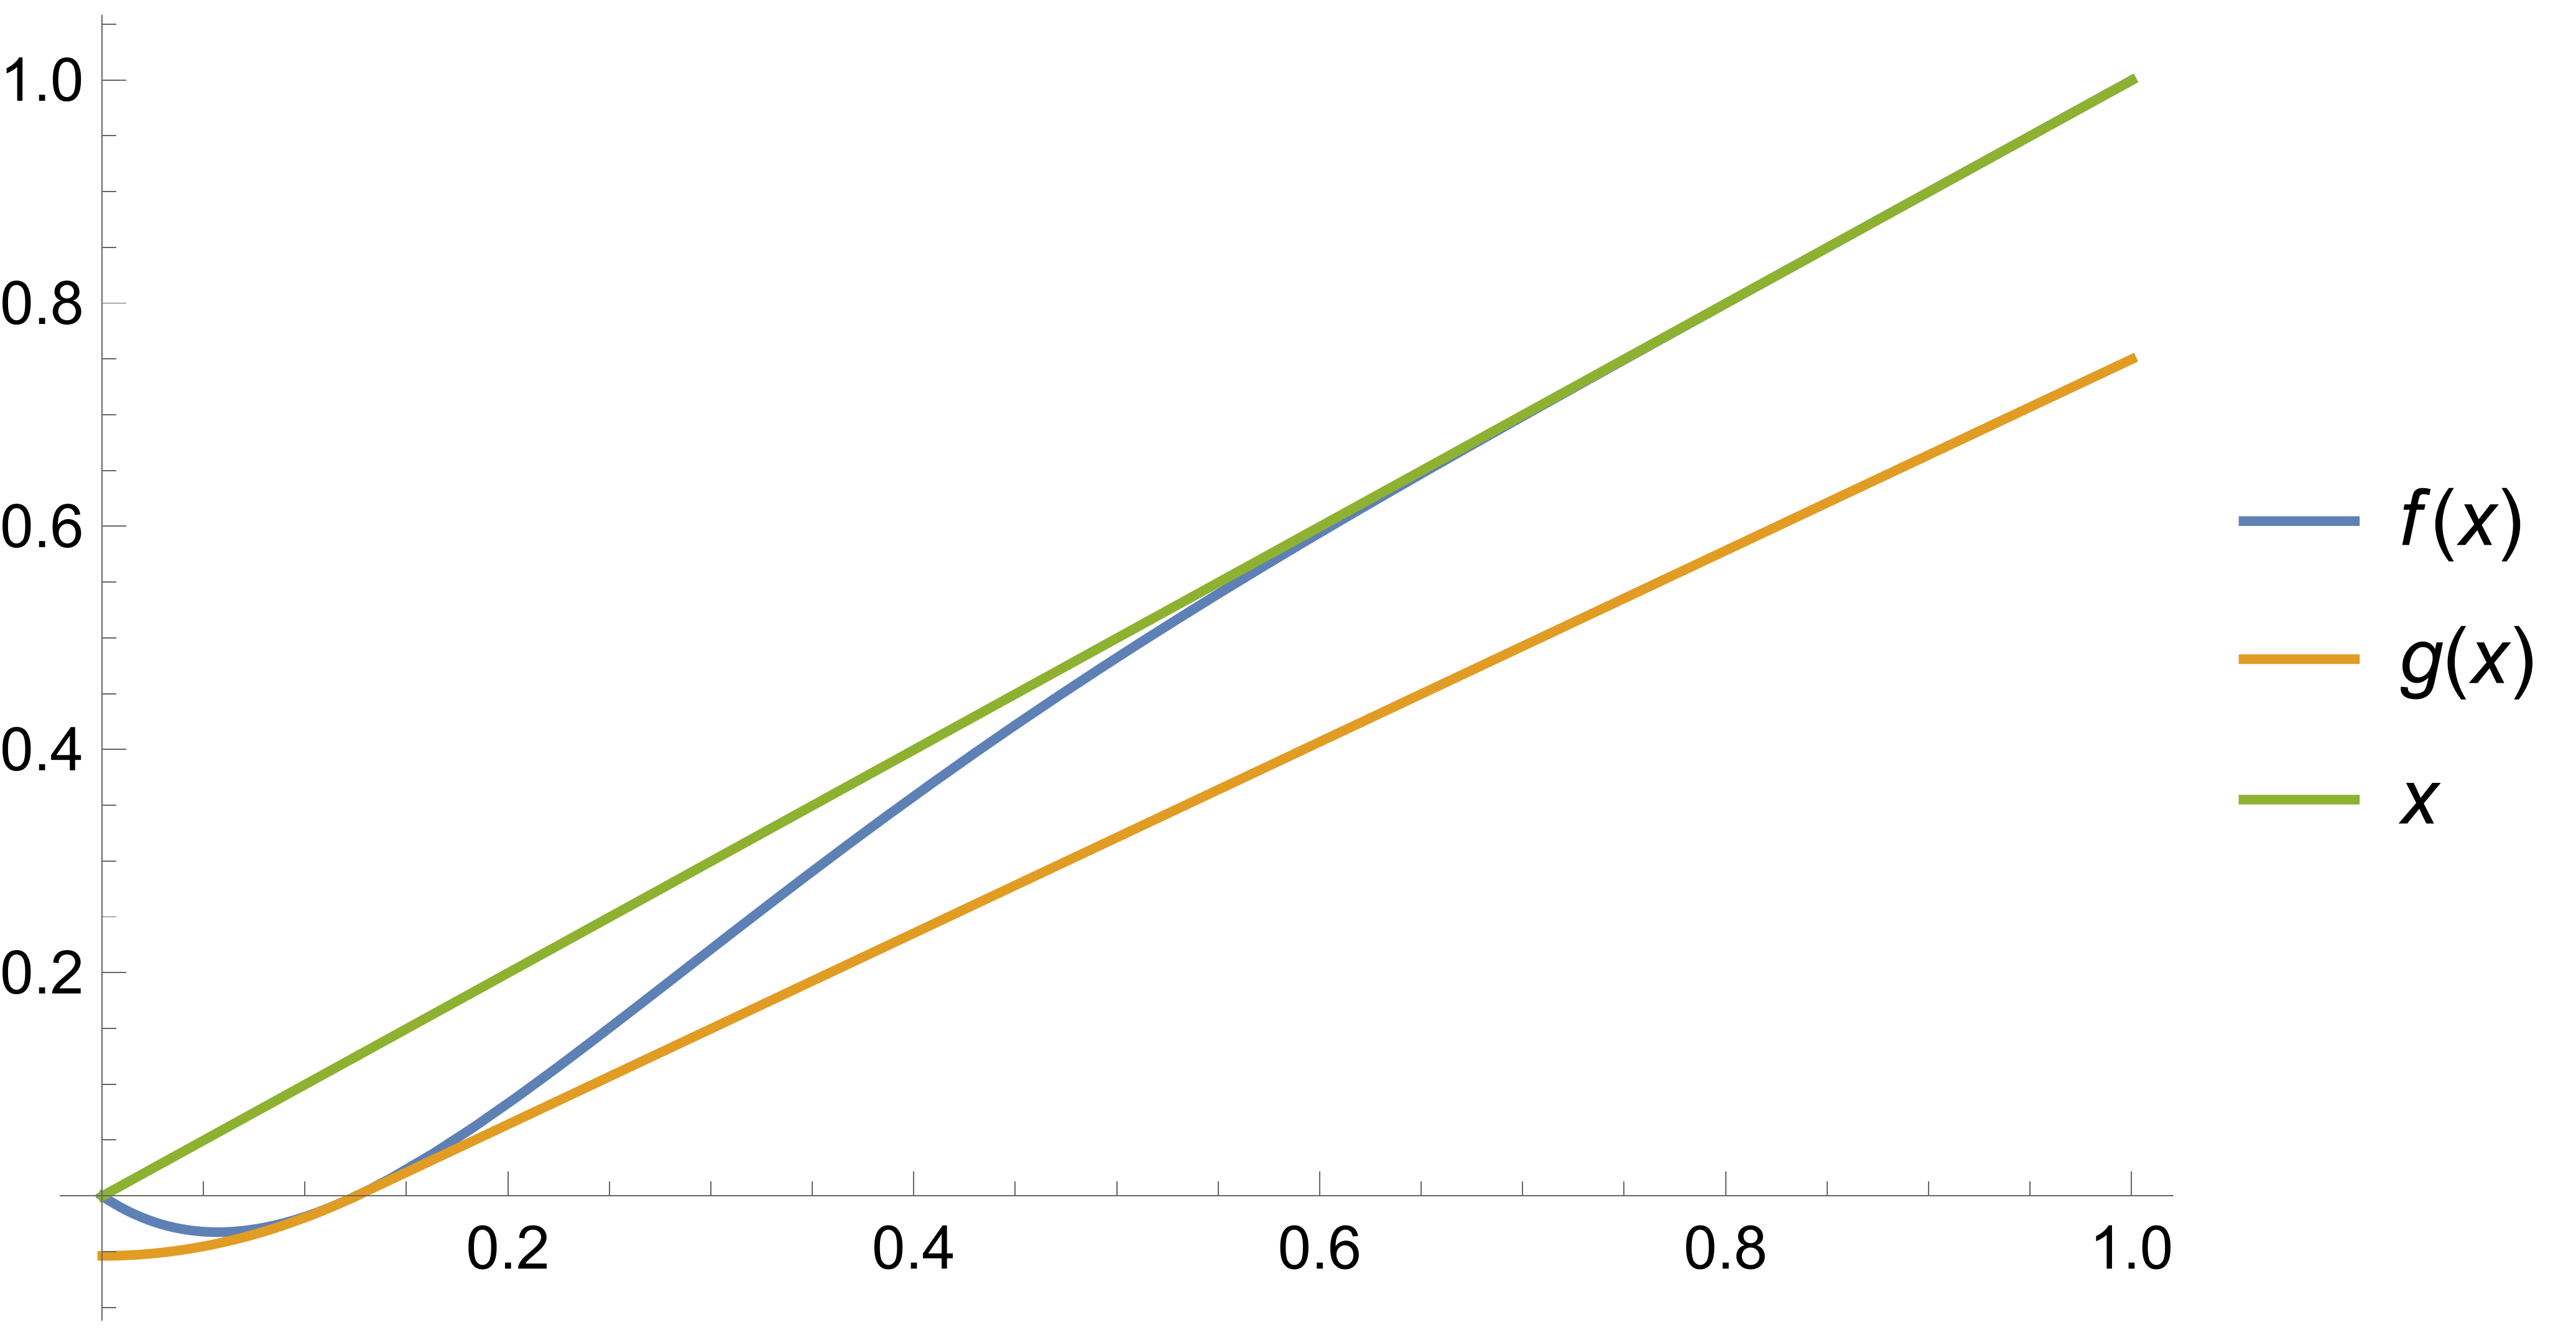
\includegraphics[width=1.0\textwidth]{figures/fig-uniformity-z2-fg}
  \caption{\label{fig:z2:fg}Our choice of $g$, here depicted for $\ab=8$, $\ns=7$.}
\end{figure}
%%%%%%%%%%%%%%%%%%%%%%%%%%%%%%%%%%%%%%%%%%%%%%%%%%%%%%%%%%%%%%%%%%%%%%%%%

To continue our analysis, we will rely on the following technical claim, whose proof is calculus and left to the reader.\exercise{You are the reader.}
\begin{claim}
Fix $\alpha\in(0,1)$ and $\beta \geq 1$ such that $\frac{\alpha\beta}{1-\alpha} \leq 1$; and define $f_{\alpha,\beta},g_{\alpha,\beta}\colon [0,1]\to\R$ by
$
f_{\alpha,\beta}(x) = x\Paren{1-\Paren{\frac{1-x}{1-\alpha}}^\beta}$ and 
\[
g_{\alpha,\beta}(x) = \frac{\alpha\beta}{1-\alpha}(x-\alpha) + \frac{\beta}{2(1-\alpha)} (x-\alpha)^2 \indic{x\leq \alpha}\,.
\]
Then $g_{\alpha,\beta}$ is nondecreasing, and $f_{\alpha,\beta}\geq g_{\alpha,\beta}$.
\end{claim}
Applying this to $\alpha\eqdef 1/\ab$ and $\beta \eqdef \ns-1$ (which, since $\ns\leq \ab$, satisfy the assumptions) leads to
\begin{align*}
  \Delta(\p) 
  &%\geq \frac{1}{4}\sum_{i\in\domain} f(\p(i)) 
  \geq \frac{1}{4}\sum_{i\in\domain} g(\p(i)) \\
  &= \frac{\ns-1}{8(1-1/\ab)} \sum_{i\in\domain} (\p(i)-1/\ab)^2\indic{\p(i)\leq 1/\ab} \\
  &\geq \frac{\ns-1}{8(\ab-1)} \Paren{\sum_{i\in\domain} \abs{\p(i)-1/\ab}\indic{\p(i)\leq 1/\ab}}^2 \\
  &= \frac{\ns-1}{8(\ab-1)} \totalvardist{\p}{\uniform_\ab}^2\,,
\end{align*}
where the first line uses $f\geq g$, the second from cancellation of the linear term of $g$, the third is Cauchy--Schwarz, and the last follows from the definition of total variation distance. Using $\ns \geq 2$ to write $\frac{\ns-1}{\ab-1}\geq \frac{\ns}{2\ab}$ concludes the proof.
\end{proof}
At this point, we have half of the puzzle: it remains to get a handle on the variance of $Z_2$ in both the far and uniform cases. We start by providing an exact (albeit unwieldy) expression for it.%, which we will then massage to obtain a usable bound in the uniform case.
\begin{align*}
\Var[Z_2] 
&= \frac{1}{\ns^2}\sum_{i,j\in\domain} \bEE{\indic{\occur_i=1}\indic{\occur_j=1}} - \bEE{Z_2}^2  \\
&= \frac{1}{\ns^2}\sum_{i\in\domain} \bEE{\indic{\occur_i=1}} + \frac{1}{\ns^2}\sum_{i\neq j} \bEE{\indic{\occur_i=1}\indic{\occur_j=1}} - \bEE{Z_2}^2 \\
&= \frac{1}{\ns}\bEE{Z_2}- \bEE{Z_2}^2 + \frac{\ns-1}{\ns}\sum_{i\neq j} \p(i)\p(j)(1-(\p(i)+\p(j)))^{\ns-2}\,, %\label{eq:var:z2}
\end{align*}
where the last line relied on~\cref{eq:def:z2} to recognize $\bEE{Z_2}$ in the first term, and on the fact that $\bEE{\indic{\occur_i=1}\indic{\occur_j=1}} = \ns(\ns-1)\p(i)\p(j)(1-(\p(i)+\p(j)))^{\ns-2}$ for $i\neq j$. (Indeed, $\indic{\occur_i=1}\indic{\occur_j=1}$ is equal to one if, and only if, out of the $\ns$ samples two fall on $i$ and $j$, respectively, and the $\ns-2$ others hit $\domain\setminus\{i,j\}$.)

This looks quite unwieldy; however, we can rearrange the term $\bEE{Z_2}^2$ to obtain the nicer expression
\begin{align}
\Var[Z_2] 
&= \frac{\bEE{Z_2}(1-\bEE{Z_2})}{\ns} + \frac{\ns-1}{\ns}\Paren{\sum_{i\neq j} \p(i)\p(j)(1-\p(i)-\p(j))^{\ns-2} - \bEE{Z_2}^2 } \notag\\
&\leq \frac{1-\bEE{Z_2}}{\ns} + \sum_{i\neq j} \p(i)\p(j)(1-\p(i)-\p(j))^{\ns-2} - \bEE{Z_2}^2 \label{eq:var:z2}
\end{align}
For the uniform case,~\cref{eq:var:z2} simplifies quite a bit, and we get
\begin{align}
\Var_{\uniform_{\ab}}[Z_2] 
%&\leq \frac{1}{\ns} \Paren{ 1-\Paren{1-\frac{1}{\ab}}^{\ns-1} } + \frac{\ab-1}{\ab}\Paren{1-\frac{2}{\ab}}^{\ns-2} - \Paren{1-\frac{1}{\ab}}^{2(\ns-1)} \notag\\
&\leq \frac{1}{\ns} \Paren{ 1-\Paren{1-\frac{1}{\ab}}^{\ns-1} } + \Paren{1-\frac{2}{\ab}}^{\ns-2} - \Paren{1-\frac{1}{\ab}}^{2(\ns-1)} \notag\\
&\leq \frac{\ns-1}{\ns\ab} + \Paren{1-\frac{1}{\ab}}^{2(\ns-2)} - \Paren{1-\frac{1}{\ab}}^{2(\ns-1)} \notag\\
&\leq \frac{1}{\ab} + \Paren{1-\frac{1}{\ab}}^{2(\ns-2)} \Paren{ 1 - \Paren{1-\frac{1}{\ab}}^{2} } \notag\\
&= \frac{1}{\ab} + \frac{2}{\ab}\Paren{1-\frac{1}{\ab}}^{2(\ns-2)} \Paren{ 1-\frac{1}{2\ab} } \leq \frac{3}{\ab}
\label{eq:var:z2:unif}
\end{align}
where the second inequality follows from $1-2x \leq (1-x)^2$, and $\Paren{1-x}^{m} \geq 1-mx$ for $m\geq 1$ and $x \leq 1$. (As a side note, we proved along the way that $\frac{1}{\ns}\Paren{1-\bE{\uniform_{\ab}}{Z_2}} \leq \frac{1}{\ab}$, which will come in handy.)

This looks great! We just proved that, at least in the uniform case, $\Var_{\uniform_{\ab}}[Z_2] \leq 3/\ab$. By the same rule of thumb as in the previous argument (\cref{eq:signal:to:noise}), we expect our test to work as long as the standard deviation (the ``noise'') of our statistic is smaller than the gap in expectations (the ``signal''), which by~\cref{lemma:gap:z2} gives the condition
\[
   \Var_{\uniform_{\ab}}[Z_2] \leq \frac{3}{\ab} \ll \frac{\dst^4\ns^2}{16\ab^2} \leq \Delta(\p)^2\,.
\]
Reorganizing, this yields the condition $\ns \gg \sqrt{\ab}/\dst^2$, which is exactly what we want to prove. The problem, of course, is that we so far only have bounded the variance in one of the two cases; to conclude, we need the last quarter of the puzzle.

To do so, we will invoke the following:
\begin{lemma}
  \label{lemma:technical:distinct:elements}
Fix $m \geq 1$ and $\ab \in \N$. For any $x_1,\dots,x_\ab \geq 0$ such that $\sum_{i=1}^\ab x_i = 1$, we have
\[
    \frac{m\sum_{1\leq i < j \leq \ab} x_i x_j \Paren{ (1-x_i - x_j)^{m-1} - (1-x_i)^m(1-x_j)^m} }{\sum_{i=1}^\ab x_i (1-(1-x_i)^m)} \leq 1
\]
\end{lemma}
Unfortunately, there is not much intuition we can provide about \emph{why} this inequality holds; and we defer its proof to the end of the chapter (\cref{sec:deferred:chap:identity}), focusing for now on how it will provide us with the last piece of said puzzle. In view of resuming from~\cref{eq:var:z2}, we expand $\bEE{Z_2}^2$ to write
\begin{align*}
\sum_{i\neq j} &\p(i)\p(j)(1-\p(i)-\p(j))^{\ns-2} - \bEE{Z_2}^2  \\
&= \sum_{i\neq j} \p(i)\p(j)(1-\p(i)-\p(j))^{\ns-2} - \sum_{i,j} \p(i)\p(j)(1-\p(i))^{\ns-1}(1-\p(j))^{\ns-1} \\
&\leq \sum_{i\neq j} \p(i)\p(j)\Paren{ (1-\p(i)-\p(j))^{\ns-2} - (1-\p(i))^{\ns-1}(1-\p(j))^{\ns-1} } \\
&\leq \frac{1}{\ns-1} \sum_{i=1}^\ab \p(i) (1-(1-\p(i))^{\ns-1}) = \frac{1-\bEE{Z_2}}{\ns-1}
\end{align*}
where the last inequality is~\cref{lemma:technical:distinct:elements} applied with $m=\ns-1$ and $x_i = \p(i)$. Then, using this in~~\cref{eq:var:z2} (and bounding $1/(\ns-1) \leq 2/\ns$) leads to 
\begin{align}
\Var[Z_2]
&\leq 3\cdot \frac{1-\bE{\p}{Z_2}}{\ns} 
= 3\Paren{ \frac{1-\bE{\uniform_{\ab}}{Z_2}}{\ns} + \frac{\bE{\uniform_{\ab}}{Z_2}-\bE{\p}{Z_2}}{\ns} }  \notag\\
&\leq 3\Paren{ \frac{1}{\ab} + \frac{\Delta(\p)}{\ns} }\,. \label{eq:var:z2:final}
\end{align}
Before invoking Chebyshev's inequality, let us see why this is wonderful news. The first term of the bound, $3/\ab$, is the same as in the uniform case, and we have discussed before how it would by itself lead to the desired sufficient condition $\ns \gg \sqrt{\ab}/\dst^2$. The second is new; by the same rule of thumb, it will lead to the condition
\[
    \frac{3\Delta(\p)}{\ns} \ll \Delta(\p)^2
\]
where one $\Delta(\p)$ crucially cancels out, leaving us with $\Delta(\p) \gg 1/\ns$. Since $\Delta(\p)\geq \frac{\dst^2\ns}{16\ab}$, a sufficient condition then becomes $\frac{\dst^2\ns}{\ab} \gg \frac{1}{\ns}$, which then will be satisfied as soon as $\ns \gg \sqrt{\ab}/\dst$.

Now that we have all the pieces of the puzzle, let us establish the main result of this subsection:
\begin{theorem}
  \label{theo:uniformity:unique:elements}
The unique-elements tester (\cref{algo:unique-elements}) is a testing algorithm for uniformity with sample complexity $\ns(\ab,\dst,1/3) = O(\sqrt{\ab}/\dst^2)$ and time complexity $O(\ns)$, provided that $\dst \geq 15/\ab^{1/4}$.
\end{theorem}
\begin{proof}
For any $\p\in\distribs{\ab}$, let as before $\Delta(\p) \eqdef \bE{\uniform_\ab}{Z_2} - \bE{\p}{Z_2}$. Of course, if $\p=\uniform_\ab$ then $\Delta(\p)=0$, and we know from~\cref{lemma:gap:z2} that $\Delta(\p) \geq \Delta \eqdef \frac{\ns\dst^2}{16\ab}$ whenever $\totalvardist{\p}{\uniform_\ab} \geq \dst$.\footnote{We assume throughout $\ns \leq \ab$, and will enforce this at the end.} We also obtained earlier (in~\cref{eq:var:z2:unif,eq:var:z2:final}) a bound in the variance of $Z_2$ in both the uniform and ``far'' cases, so we have all the ingredients we need. Define our threshold
\[
    \tau \eqdef \bE{\uniform_\ab}{Z_2} - \frac{\Delta}{2}
\]
as in~\cref{algo:unique-elements}.
\begin{itemize}
    \item In the uniform case, the probability to output \reject (and thus make a mistake) is bounded as
    \[
    \bPr{Z_2 \leq \tau} = \bPr{Z_2 \leq \bE{\uniform_\ab}{Z_2} - \frac{\Delta}{2} } \leq \frac{4\Var_{\uniform_\ab}[Z_2]}{\Delta^2}
    \leq \frac{3072\ab}{\dst^4\ns^2}
    \]
    by Chebyshev's inequality, using $\Var_{\uniform_\ab}[Z_2] \leq 3/\ab$ and the definition of $\Delta$. This in turn is less than $1/3$ as long as $\ns \geq 96\sqrt{\ab}/\dst^2$.
    \item In the ``far'' case, since $\bE{\p}{Z_2} = \bE{\uniform_\ab}{Z_2} - \Delta(\p)$ and $\Delta(\p) \geq \Delta$ the probability to err by outputting \accept is
    \begin{align*}
        \bPr{Z_2 > \tau} &= \bPr{Z_2 > \bE{\p}{Z_2} + \frac{\Delta(\p)}{2} + \frac{\Delta(\p)-\Delta}{2} } \\       
        &\leq \bPr{Z_2 > \bE{\p}{Z_2} + \frac{\Delta(\p)}{2} } \\
        &\leq \frac{4\Var_{\p}[Z_2]}{\Delta(\p)^2} 
        \leq \frac{12}{\ab \Delta(\p)^2} + \frac{12}{\ns \Delta(\p)} \\
        &\leq \frac{3072\ab}{\dst^4\ns^2} + \frac{192\ab}{\dst^2\ns^2} \leq \frac{3264\ab}{\dst^4\ns^2}
    \end{align*}
    using $\Var_{\p}[Z_2] \leq 3/\ab+3\Delta(\p)/\ns$. The resulting bound is then less than $1/3$ for $\ns \geq 99\sqrt{\ab}/\dst^2$.
  \end{itemize}
  The above analysis shows that both errors are less than $1/3$ for, say, $\ns = \lceil{99\sqrt{\ab}/\dst^2}\rceil$. However, we did rely on~\cref{lemma:gap:z2}, which requires $\ns \leq \ab$; given our choice of $\ns$, this in turns imposes a condition on $\dst$ (for instance, one can check that $\dst \geq 15/\ab^{1/4}$ suffices).
\end{proof}

%%%%%%%%%%%%%%%%%%%%%%%%%%%%%%%%%%%%%%%%%%%%%%%%%%%%%%%%%%%%%%%%%%%%%%%%%
\subsection{Modified $\chi^2$}
  \label{ssec:uniformity:chisquare}  If you are a statistician, or just took a Statistics class, or even got lost on Wikipedia at some point and ended up on the wrong page at the wrong time, you may know of Pearson's $\chi^2$ test for goodness-of-fit: for every element $i$ of the domain, count how many times it appeared in the samples, $\occur_i$. Compute $\sum_{i} \frac{(\occur_i-\ns/\ab)^2}{\ns/\ab}$. Compare the result to a predetermined threshold. This very natural idea, maybe not surprisingly, works well! In particular, since $\occur_i \sim \binomial{\ns}{\p(i)}$, one can derive
\[
\bEE{ \sum_{i=1}^\ab \frac{(\occur_i-\ns/\ab)^2}{\ns/\ab} } = \frac{\ab}{\ns}\sum_{i=1}^\ab \bEE{ \Paren{\occur_i-\frac{\ns}{\ab}}^2 } = \ab(\ns-1)\normtwo{\p-\uniform_\ab}^2 + \ab-1\,,
\]
using moments of a Binomial random variable and~\cref{eq:relation:collisionprob:distance:uniform}.\exercise{Check it!} This does look like a reasonable way to estimate the distance to uniformity \emph{via} the $\lp[2]$ distance again\dots{} unfortunately, the variance will be quite annoying, due to the correlations between terms of the sums.

To make the task easier, it is helpful to think of taking $\poisson{\ns}$ samples instead of exactly $\ns$, which will greatly simplify the analysis. Then, under this (slightly different) sampling model the $\occur_i$'s become independent, with $\occur_i\sim\poisson{\ns\p(i)}$: this is called \emph{Poissonization}\index{Poissonization}, and can be done more or less without loss of generality since a $\poisson{\ns}$ random variable will be between $0.99\ns$ and $1.01\ns$ with overwhelming probability. (See~\cref{app:poissonization} for more on Poissonization, and why we can use it ``without loss of generality'').

\begin{algorithm}[ht!]
  \begin{algorithmic}[1]
    \Require Multiset of $\ns$ samples $x_1,\dots,x_\ns \in \domain$, parameters $\dst\in(0,1]$ and $\ab = \abs{\domain}$
    \Comment{Assumes Poissonization}
    \State Set $\tau \gets 2\ns\dst^2$
    \State Compute \Comment{Can be done in $O(\ns)$ time if $\domain$ is known, $O(\ns\log\ns)$ if only $\ab$ is.}
    \[
        Z_3 = \sum_{j\in\domain} \frac{(\occur_j-\ns/\ab)^2-\occur_j}{\ns/\ab}
    \] where $\occur_j \gets \sum_{t=1}^\ns\indic{x_t=j}$.
    \If{ $Z_3 \geq \tau$ } \Return \reject \Comment{Not uniform}
    \Else\ 
      \Return \accept \Comment{Uniform}
    \EndIf
  \end{algorithmic}
  \caption{\label{algo:chisquare}\sc Chi-Square Tester}
\end{algorithm}

The bad news is that it does not actually lead to the optimal sample complexity: Poissonization introduces a bit more variance (as we introduce extra randomness ourselves by taking a random number of samples), and so the variance of this $\chi^2$ test can be too big due to the elements we only expect to see zero or once (so, most of them). The \emph{good} news is that a simple correction of that test, of the form
\begin{equation}
  \label{eq:def:z3}
    Z_3 = \sum_{i=1}^\ab \frac{(\occur_i-\ns/\ab)^2- \occur_i}{\ns/\ab}
\end{equation}
\emph{does} have a much smaller variance, and a threshold test of the form ``$Z_3 > \tau$?'' will yield the right sample complexity.\footnote{In the multinomial (``non-Poissonized'') case, substracting $\occur_i$ was not necessary, since that would correspond to removing overall $\frac{\ab}{\ns}\sum_{i=1}^\ab \occur_i = \ab$, a constant term. In the Poissonized case, however, $\sum_{i=1}^\ab \occur_i\sim\poisson{\ns}$, and $\frac{\ab}{\ns}\sum_{i=1}^\ab \occur_i$ is not a constant -- it is a random variable with expectation $\ab$ and (large) variance $\ab^2/\ns$.} Recalling that $\occur_i\sim\poisson{\ns\p(i)}$ for all $i$, the expectation of $Z_3$ will then just be 
\begin{equation}
  \label{eq:expectation:z3}
    \expect{Z_3} = \ns\ab \normtwo{\p-\uniform_\ab}^2
\end{equation}
which is perfect. Analyzing this test boils down, again, to bounding the variance of $Z_3$ and invoking Chebyshev's inequality\dots{} Before doing so, we will make a change which looks innocuous, but will come in quite handy in~\cref{sec:identity} when generalizing beyond the uniform distribution: let us rewrite
\[
    Z_3 = \sum_{i=1}^\ab \frac{(\occur_i-\ns\uniform_\ab(i))^2- \occur_i}{\ns\uniform_\ab(i)}
\]
where, of course, $\uniform_\ab(i) = 1/\ab$ for all $i\in[\ab]$. Recalling that, by Poissonization, all the $\occur_i$'s are independent Poisson random variables, we will invoke the technical claim below, which follows from (somewhat tedious, but straightforward) computations involving the moments of Poisson random variables:\exercise{Verify it: \cref{ex:uniformity:moments:poisson}.}
\begin{claim}
  \label{claim:uniformity:moments:poisson}
  Let $\mu, \lambda \geq 0$. If $X\sim\poisson{\lambda}$, then 
  $
  \bEE{(X-\mu)^2-X} = (\lambda-\mu)^2
  $
  and 
  $
  \bEE{((X-\mu)^2-X)^2} = (\lambda-\mu)^4 + 2\lambda^2 + 4\lambda(\lambda-\mu)^2
  $.
\end{claim}
Given this, by linearity of expectation we immediately get\footnote{Here, $\chisquare{\p}{\q} = \sum_{i=1}^\ab\frac{(\p(i)-\q(i))^2}{\q(i)}$ denotes the \emph{chi-square divergence} between distributions $\p$ and $\q$; for a refresher on this notion of distance, the reader is referred to~\cref{app:distances}.}
\begin{align}
    \bEE{Z_3} 
    &= \sum_{i=1}^\ab \frac{\bEE{(\occur_i-\ns\uniform_\ab(i))^2- \occur_i}}{\ns\uniform_\ab(i)}
    = \ns\sum_{i=1}^\ab \frac{(\p(i)-\uniform_\ab(i))^2}{\uniform_\ab(i)} \notag\\
    &= \ns\cdot\chisquare{\p}{\uniform_\ab} \label{eq:expectation:z3:chisquare}
\end{align}
which here can further be simplified by $\chisquare{\p}{\uniform_\ab} = \ab\normtwo{\p-\uniform_\ab}^2$, as the denominator is constant and equal to $1/\ab$; this establishes~\cref{eq:expectation:z3}.

Turning to the variance, we want to relate $\Var[Z_3]$ to known quantities, and in particular $\bEE{Z_3}$. To do so, we use independence of the $\occur_i$'s followed by the second part of the above claim to get
\begin{align}
    \Var[Z_3]
    &= \sum_{i=1}^\ab \frac{\Var[(\occur_i-\ns\uniform_\ab(i))^2- \occur_i]}{\ns^2\uniform_\ab(i)^2} \notag\\
    &= \sum_{i=1}^\ab \frac{2\ns^2\p(i)^2 + 4\ns^3\p(i)(\p(i)-\uniform_\ab(i))^2}{\ns^2\uniform_\ab(i)^2} \notag\\
    &= 2\sum_{i=1}^\ab \frac{\p(i)^2}{\uniform_\ab(i)^2}+4\ns\sum_{i=1}^\ab \frac{\p(i)(\p(i)-\uniform_\ab(i))^2}{\uniform_\ab(i)^2}\notag\\
    &\leq 2\sum_{i=1}^\ab \frac{\p(i)^2}{\uniform_\ab(i)^2}+4\ns\sqrt{\sum_{i=1}^\ab \frac{\p(i)^2}{\uniform_\ab(i)^2}}\cdot\sqrt{\sum_{i=1}^\ab \frac{(\p(i)-\uniform_\ab(i))^4}{\uniform_\ab(i)^2}}\notag\\
    &\leq 2\sum_{i=1}^\ab \frac{\p(i)^2}{\uniform_\ab(i)^2}+4\ns\sqrt{\sum_{i=1}^\ab \frac{\p(i)^2}{\uniform_\ab(i)^2}}\cdot\sum_{i=1}^\ab \frac{(\p(i)-\uniform_\ab(i))^2}{\uniform_\ab(i)}\notag\\
    &= 2\sum_{i=1}^\ab \frac{\p(i)^2}{\uniform_\ab(i)^2} + 4\sqrt{\sum_{i=1}^\ab \frac{\p(i)^2}{\uniform_\ab(i)^2}}\bEE{Z_3} \label{eq:z3:var:interm}\,,
\end{align}
where the first inequality is Cauchy--Schwarz, and the second is monotonicity of $\lp[p]$ norms: namely, $\lp[2] \leq \lp[1]$. In order to proceed further, we need to bound the quantity $\sum_{i=1}^\ab \frac{\p(i)^2}{\uniform_\ab(i)^2}$. The trick here will be to write, using $(a+b)^2 \leq 2a^2+2b^2$, 
\[
    \p(i)^2 = ((\p(i)-\uniform_\ab(i))+\uniform_\ab(i))^2 \leq 2(\p(i)-\uniform_\ab(i))^2 + 2\uniform_\ab(i)^2\,,
\]
since then we have
\begin{align*}
    \sum_{i=1}^\ab \frac{\p(i)^2}{\uniform_\ab(i)^2}
    &\leq 2\ab + 2\sum_{i=1}^\ab \frac{(\p(i)-\uniform_\ab(i))^2}{\uniform_\ab(i)^2}  
    = 2\ab + 2\ab\sum_{i=1}^\ab \frac{(\p(i)-\uniform_\ab(i))^2}{\uniform_\ab(i)} \\
    &= 2\ab\Paren{ 1 + \frac{\bEE{Z_3}}{\ns}  }\,.
\end{align*}
Putting this back in~\cref{eq:z3:var:interm}, we get
\begin{equation}
    \Var[Z_3]
    \leq 4\ab\Paren{ 1 + \frac{\bEE{Z_3}}{\ns}  } + 4\sqrt{2}\ab^{1/2}\bEE{Z_3}+4\sqrt{2}\frac{\ab^{1/2}}{\ns^{1/2}} \bEE{Z_3}^{3/2} \label{eq:z3:var}
\end{equation}
In particular, in the uniform case $\bE{\uniform_\ab}{Z_3} = 0$, and so $\Var_{\uniform_\ab}[Z_3] \leq 4\ab$. Before formally analyzing the resulting sample complexity via (once more) Chebyshev's inequality, let us do the usual check and compare standard deviation (noise) to expectation gap (signal), and see if things look promising. The gap in expectation will be, given~\cref{eq:expectation:z3:chisquare}, at least $\Delta \eqdef \ns\ab \cdot \frac{4\dst^2}{\ab} = 4\ns\dst^2$; so, in the uniform case, we need
$\Var_{\uniform_\ab}[Z_3] \ll \Delta^2$ which, given the above, is satisfied as long as $\ns \gg \sqrt{\ab}/{\dst^2}$, since then
\[
    \Var_{\uniform_\ab}[Z_3] \leq 4\ab \ll 16\ns^2\dst^4 \leq \Delta^2\,.
\]
In the ``far'' case, for $\p$ at total variation distance at least $\dst$ from uniform, the condition is $\Var_\p[Z_3] \ll \Delta(\p)^2 = \bE{\p}{Z_3}^2$, which by~\cref{eq:z3:var} will require
\[
    \max\Paren{\ab, \frac{\ab}{\ns}\bE{\p}{Z_3}, \ab^{1/2}\bE{\p}{Z_3} , \frac{\ab^{1/2}}{\ns^{1/2}}\bE{\p}{Z_3}^{3/2} } \ll \bE{\p}{Z_3}^2\,.
\]
Considering each term separately, simplifying, and recalling that $\bE{\p}{Z_3} \geq 4\ns\dst^2$, we see that this will also hold as long as $\ns \gg \sqrt{\ab}/{\dst^2}$.

We will make this formal, and show the following:
\begin{theorem}
  \label{theo:z3}
The $\chi^2$-based tester (\cref{algo:chisquare}) is a testing algorithm for uniformity with sample complexity $\ns(\ab,\dst,1/3) = O(\sqrt{\ab}/\dst^2)$ and time complexity $O(\ns)$ in the Poissonized setting.
\end{theorem}
\begin{proof}
For any $\p\in\distribs{\ab}$, let as before $\Delta(\p) \eqdef \bE{\p}{Z_3}$. By~\cref{eq:expectation:z3}, we know that if $\p=\uniform_\ab$ then $\Delta(\p)=0$, and that $\Delta(\p) \geq \Delta \eqdef 4\ns\dst^2$ whenever $\totalvardist{\p}{\uniform_\ab} \geq \dst$ (recalling~\cref{eq:relation:l1:l2:cs}). We also have our variance bound from~\cref{eq:z3:var}. Define our threshold
\[
    \tau \eqdef \frac{\Delta}{2}
\]
as in~\cref{algo:chisquare}.
\begin{itemize}
    \item In the uniform case, where $\bE{\uniform_\ab}{Z_3}=0$, the probability to output \reject (and thus make a mistake) is bounded as
    \[
    \bPr{Z_3 \geq \tau} \leq \frac{4\Var_{\uniform_\ab}[Z_3]}{\Delta^2}
    \leq \frac{\ab}{\dst^4\ns^2}
    \]
    by Chebyshev's inequality, using $\Var_{\uniform_\ab}[Z_3] \leq 4\ab$ and the definition of $\Delta$. This in turn is less than $1/3$ as long as $\ns \geq \sqrt{3\ab}/\dst^2$.
    \item In the ``far'' case, since $\bE{\p}{Z_3} \geq \Delta$ the probability to err by outputting \accept is
    \begin{align*}
        \bPr{Z_3 < \tau} %&= \bPr{Z_3 < \frac{\Delta(\p)}{2}  } \\       
        &\leq \bPr{\abs{Z_3 - \bE{\p}{Z_3}} > \frac{\Delta(\p)}{2} } \\
        &\leq \frac{4\Var_{\p}[Z_3]}{\Delta(\p)^2} \\
        &\leq \frac{16\ab\Paren{ 1 + \frac{\bEE{Z_3}}{\ns}  } + 16\sqrt{2}\ab^{1/2}\bEE{Z_3}+16\sqrt{2}\frac{\ab^{1/2}}{\ns^{1/2}} \bEE{Z_3}^{3/2}}{\bEE{Z_3}^2} \\
        %&= \frac{16\ab}{\bEE{Z_3}^2} + \frac{16\ab}{\ns\bEE{Z_3}^{\vphantom{2}}} + \frac{16\sqrt{2}\ab^{1/2}}{\bEE{Z_3}^{\vphantom{2}}}+\frac{16\sqrt{2}\ab^{1/2}}{\ns^{1/2}\bEE{Z_3}^{1/2}} \\
        &\leq \frac{\ab}{\ns^2\dst^4} + \frac{4\ab}{\ns^2\dst^2} + \frac{4\sqrt{2}\ab^{1/2}}{\ns\dst^2}+\frac{8\sqrt{2}\ab^{1/2}}{\ns\dst} \\
        &\leq \frac{5\ab}{\ns^2\dst^4} + \frac{12\sqrt{2}\ab^{1/2}}{\ns\dst^2}
    \end{align*}
    first using~\cref{eq:z3:var}, simplifying, then $\bEE{Z_3}\geq \ns\dst^2$. By solving the inequality $5x^2 + 12\sqrt{2}x \leq 1/3$, we see that the result is at most $1/3$ for $\ns \geq 52\sqrt{\ab}/\dst^2$.
  \end{itemize}
  The above analysis shows that both errors are less than $1/3$ for, say, $\ns = \lceil{52\sqrt{\ab}/\dst^2}\rceil$; this concludes the proof.
\end{proof}

% It's a good exercise, and under the Poissonization assumption not that hard. (Try \emph{without} removing $\occur_i$ in the numerator, though, and see what you get\dots)

%%%%%%%%%%%%%%%%%%%%%%%%%%%%%%%%%%%%%%%%%%%%%%%%%%%%%%%%%%%%%%%%%%%%%%%%%
\subsection{Empirical distance to uniform}
  \label{sec:uniformity:empirical}
 Let us take a break from $\lp[2]$ and consider another, very natural thing to try: the \emph{plugin estimator}. Since we have $\ns$ samples from $\p$, we can compute the empirical estimator of the distribution, $\hat{\p}_\ns$, based on these $\ns$ samples. Now, we want to test $\totalvardist{\p}{\uniform_\ab}=0$ vs. $\totalvardist{\p}{\uniform_\ab}>\dst$? Why not consider 
\begin{equation}
    Z_4 \eqdef \totalvardist{\hat{\p}}{\uniform_\ab}
\end{equation}
the empirical distance to uniform? A reason might be: \emph{this sounds like a terrible idea.} Unless $\ns = \Omega(\ab)$ (which is much more than what we want), we will not have observed most of the domain elements even once, and the empirical distribution $\hat{\p}_\ns$ will be at distance $1-o(1)$ from uniform, \emph{even} if $\p$ is actually uniform. 

That's the thing, though: the devil is in the $o(1)$ details. Sure, $\expect{Z_4}$ will be \emph{almost} $1$ whether $\p$ is uniform or far from it unless $\ns = \Omega(\ab)$. But this ``almost'' will be different in the two cases! Carefully analyzing this tiny gap in expectation, and showing that $Z_4$ concentrates well enough around its expectation to preserve this tiny gap, amazingly leads to a tester with optimal sample complexity $\ns = \Theta(\sqrt{\ab}/\dst^2)$. Let us see how.

\begin{algorithm}[ht!]
  \begin{algorithmic}[1]
    \Require Multiset of $\ns$ samples $x_1,\dots,x_\ns \in \domain$, parameters $\dst\in(0,1]$ and $\ab = \abs{\domain}$
    \LineComment{Set the threshold $\tau$, depending on the parameter regime.}
    \If{ $\ns \leq \ab$ }
        \State $\tau \gets \frac{\ns^2\dst^2}{32e\ab^2}$
    \ElsIf{$\ab < \ns \leq \ab/\dst^2$}
        \State $\tau \gets c_1\cdot \dst^2\sqrt{\ns/\ab}$ \Comment{$c_1>0$ is some absolute constant.}
    \Else
        \State $\tau \gets c_2\cdot\dst$ \Comment{$c_2>0$ is some absolute constant.}
    \EndIf
    \State Compute \Comment{Can be done in $O(\ns)$ time if $\domain$ is known, $O(\ns\log\ns)$ if only $\ab$ is.}
    \[
        Z_4 = \totalvardist{\hat{\p}}{\uniform_\ab} = \frac{1}{2} \sum_{j=1}^\ab \abs{\frac{\occur_j}{\ns} - \frac{1}{\ab} }
    \] where $\occur_j \gets \sum_{t=1}^\ns\indic{x_t=j}$.
    \If{ $Z_4 \geq \bE{\uniform_\ab}{Z_4} + \tau$ } \Return \reject \Comment{Not uniform}
    \Else\ 
      \Return \accept \Comment{Uniform}
    \EndIf
  \end{algorithmic}
  \caption{\label{algo:empirical:plugin}\sc empirical-distance tester}
\end{algorithm}

For simplicity of exposition, we focus here on the case $\ns \leq \ab$, though the analysis of the test can be extended to all parameter regimes~--~see~\citet{DiakonikolasGPP18} for the full general case. The argument proceeds in two steps: first, computing and bounding the expectation of $Z_4$ under the uniform and the far cases separately is not going to really work, so instead we will bound the expectation gap $\Delta(\p)\eqdef \bE{\p}{Z_4}-\bE{\uniform_{\ab}}{Z_4}$ directly (a little like in the case of the unique elements-based tester). Then, once the gap in expectation is established, we will once again argue concentration of $Z_4$ as usual by a variance-based (Chebyshev's inequality) argument~--~but this time diversifying our toolkit and using a different tool, the Efron--Stein lemma, to bound the variance.
%instead by invoking a more powerful (and slightly fancier) concentration inequality.\todonote{Revisit this.}

\paragraph{The expectation gap $\Delta(\p)$.} From the definition of total variation distance, we can rewrite
\[
    Z_4 = \sum_{i=1}^\ab \Paren{\hat{\p}_\ns(i) - \frac{1}{\ab}}\indic{\hat{\p}_\ns(i) > 1/\ab}
    = \frac{1}{\ns} \sum_{i=1}^\ab \Paren{\occur_i - \frac{\ns}{\ab} }_+
\]
where as previously $\occur_i$ denotes the number of samples falling on element $i$, and $x_+ \eqdef \max(x,0)$. For the sake of the analysis, we will introduce the multivariate function
\begin{equation}
  \label{eq:empirical:S}
  S(x_1,\dots,x_\ns) \eqdef \frac{1}{\ns} \sum_{i=1}^\ab \Paren{\occur_i(x_1,\dots,x_\ns) - \frac{\ns}{\ab} }_+
\end{equation}
and the function $\mu\colon\distribs{\ab}\to \R$ given by
\[
 \mu(\p) \eqdef \bE{\p}{S(X_1,\dots,X_\ns)}\,.
\] 
(Note that $\bE{\p}{Z_4} = \mu(\p)$.) Then, since $\occur_i\sim\binomial{\ns}{\p(i)}$ under $\p$, we have the exact expression
\begin{align*}
 \mu(\p) 
    &= \frac{1}{\ns} \sum_{i=1}^\ab \sum_{\ell=0}^\ns \binom{\ns}{\ell} \p(i)^\ell (1-\p(i))^{\ns-\ell} \Paren{\ell - \frac{\ns}{\ab} }_+ \\
    &= \frac{1}{\ns} \sum_{i=1}^\ab \sum_{\ell=1}^\ns \binom{\ns}{\ell} \p(i)^\ell (1-\p(i))^{\ns-\ell} \Paren{\ell - \frac{\ns}{\ab} }
\end{align*}
since $\Paren{\ell - \ns/\ab }_+ > 0$ for $\ell \geq \clg{\ns/\ab}=1$ (recall that we assume $\ns \leq \ab$). Using the facts that
$
    \sum_{\ell=0}^\ns \binom{\ns}{\ell} \p(i)^\ell (1-\p(i))^{\ns-\ell} = 1
$
and
$
    \sum_{\ell=0}^\ns \ell \binom{\ns}{\ell} \p(i)^\ell (1-\p(i))^{\ns-\ell} = \ns\p(i)
$, the inner sum considerably simplifies and we get
\begin{align}
  \label{eq:empirical:tv:mu}
 \mu(\p) 
    &= \frac{1}{\ab} \sum_{i=1}^\ab (1-\p(i))^{\ns}
\end{align}
Since our goal is to lower bound $\Delta(\p) = \mu(\p) - \mu(\uniform_\ab)$, the view of $\mu$ as a multivariate function suggests a Taylor expansion around $\mu(\uniform_\ab)$. Namely, for any $\p\in\distribs{\ab}$, we can write by Taylor's theorem
\[
    \mu(\p) = \mu(\uniform_\ab) + \grad{\mu(\uniform_\ab)}^\top (\p-\uniform_\ab) + \frac{1}{2} (\p-\uniform_\ab)^\top \mathbf{H}(\q) (\p-\uniform_\ab)
\]
where $\q = (1-\theta)\uniform_\ab+\theta\p$ for some $\theta\in[0,1]$, and $\mathbf{H}$ is the Hessian of $\mu$: $\mathbf{H}_{i,j}(\q) = \pdv{\mu}{x_i}{x_j}\-(\q)$.  Given~\cref{eq:empirical:tv:mu}, we can compute explicitly both the gradient and the Hessian: first, denoting by $\mathbf{1}_{\ab}$ the all-one vector,
\[
    \grad{\mu(\uniform_\ab)} = \Paren{\pdv{\mu}{x_1}\-(\uniform_\ab),\dots,\pdv{\mu}{x_\ab}\-(\uniform_\ab) } = -\frac{\ns}{\ab}\Paren{ 1-\frac{1}{\ab} }^{\ns-1} \mathbf{1}_{\ab}
\]
so  
$
\grad{\mu(\uniform_\ab)}^\top (\p-\uniform_\ab) = -\frac{\ns}{\ab}(1-\frac{1}{\ab})^{\ns-1} \sum_{i=1}^\ab (\p(i)-\frac{1}{\ab}) = 0
$. Then, as $\mu$ is separable, $\mathbf{H}$ will be diagonal: $\mathbf{H}_{i,j}(\q) = 0$ for $i\neq j$, while
\[
    \mathbf{H}_{i,i}(\q) = \frac{\ns(\ns-1)}{\ab}(1-\q(i))^{\ns-2}
\]
for all $i\in[\ab]$. Recalling our Taylor expansion, this means that
\begin{align}
    \Delta(\p) 
    &= \frac{1}{2} (\p-\uniform_\ab)^\top \mathbf{H}(\q) (\p-\uniform_\ab) \notag\\
    &= \frac{\ns(\ns-1)}{2\ab}\sum_{i=1}^\ab (1-\q(i))^{\ns-2} \Paren{\p(i)-\frac{1}{\ab}}^2
\end{align}
where again $\q$ is a probability distribution such that $\q = (1-\theta)\uniform_\ab+\theta\p$ for some $\theta\in[0,1]$. To proceed, a natural idea is to restrict the sum to indices for which we can non-trivially bound $(1-\q(i))^{\ns-2}$; in particular, focusing on the indices $i$ for which $\p(i) < 1/\ab$ will do, since for those we must have $\q(i) \leq 1/\ab$ as well. This leads to writing
\begin{align}
    \Delta(\p) 
    &\geq \frac{\ns(\ns-1)}{2\ab}\sum_{i=1}^\ab (1-\q(i))^{\ns-2} \Paren{\p(i)-\frac{1}{\ab}}^2 \indic{\p(i) < 1/\ab} \notag\\
    &\geq \frac{\ns(\ns-1)}{2\ab}\Paren{1-\frac{1}{\ab}}^{\ns-2} \sum_{i=1}^\ab \Paren{\p(i)-\frac{1}{\ab}}^2 \indic{\p(i) < 1/\ab} \notag\\
    &\geq \frac{\ns(\ns-1)}{2\ab}\Paren{1-\frac{1}{\ab}}^{\ns-2} \frac{1}{\ab}\Paren{\sum_{i=1}^\ab \Paren{\frac{1}{\ab}-\p(i)} \indic{\p(i) < 1/\ab}}^2 \notag\\
    &\geq \frac{\ns(\ns-1)}{2\ab^2}\Paren{1-\frac{1}{\ab}}^{\ab-2} \dst^2 
    \geq \frac{\ns^2\dst^2}{4e\ab^2} \label{eq:empirical:expectation:gap}
\end{align}
where the third inequality is Cauchy--Schwarz, the fourth is the definition of total variation distance along with $\totalvardist{\p}{\uniform_\ab}\geq \dst$ (and, in the exponent, $\ns \leq \ab$), and the last is $\Paren{1-1/\ab}^{\ab-2} \geq 1/e$ for $\ab \geq 2$.

Before turning to proving concentration of $Z_4$ (that is, showing that the expectation gap, our signal, is not drowned by the random fluctations of $Z_4$ around its expectation), we will make an observation which will help in the analysis. Since we restricted ourselves to the regime $\ns/\ab\leq 1$, the $i$-th summand of $S$ in~\cref{eq:empirical:S} is non-zero only when $\occur_i\geq 1$, and thus we can rewrite
\begin{align}
  Z_4
  &= \frac{1}{\ns} \sum_{i=1}^\ab \Paren{ \Paren{ \occur_i - \frac{\ns}{\ab} } +  \frac{\ns}{\ab} \indic{\occur_i = 0} } \notag\\
  &= \frac{1}{\ns} \sum_{i=1}^\ab \Paren{ \occur_i - \frac{\ns}{\ab} } + \frac{1}{\ab} \sum_{i=1}^\ab \indic{\occur_i = 0} \notag\\
  &= \frac{1}{\ab} \sum_{i=1}^\ab \indic{\occur_i = 0} \label{eq:empirical:S:alt}
\end{align}
where the last equality follows from $\sum_{i=1}^\ab \occur_i = \ns$. 
That is, in this regime, $Z_4$ is exactly the fraction of \emph{unseen elements} of the domain; this readily allows one to retrieve~\cref{eq:empirical:tv:mu}, and also lets us relate $Z_4$ to the ``unique elements'' statistic $Z_2$ from~\cref{sec:uniformity:unique}.\footnote{Again, this relation only holds in the specific regime $\ns \leq \ab$; while we do not cover the case $\ns > \ab$ here, the guarantees of $Z_4$ extend to this other regime; the identity~\cref{eq:empirical:S:alt}, however, does not.}

\paragraph{Concentration of $Z_4$.} As you may have guessed, we will show that $Z_4$ concentrates around its expectation via Chebyshev's inequality, which requires us to bound $\Var[Z_4]$ in both the uniform and ``far'' cases. In order to diversify our toolkit, we will do so by invoking the \emph{Efron--Stein inequality}\index{Efron--Stein inequality}, which allows us to bound the variance of a function of $\ns$ independent random variables by the expected quadratic change of this function when only one sample is re-randomized: for a function $f$ of $\ns$ variables,
\begin{align}
    \Var[ f(X)]  \leq \frac{1}{2} \sum_{t=1}^\ns \bEE{ \Paren{ f(X) - f(X^{(t)}) }^2 }
\end{align}
where $X=(X_1\dots,X_\ns)$ and $X^{(t)} = (X_1,\dots, X'_t, \dots, X_\ns)$, with $X'_t$ being an independent copy of $X_t$.

We apply this to $Z_4$, \ie the function $S$ defined in~\cref{eq:empirical:S}; given that $S$ is symmetric and that all $X_t$'s are \iid and distributed according to $\p$, we get
\begin{align*}
  \Var[Z_4] 
  &\leq \frac{\ns}{2}  \bE{\p}{ \Paren{ S(X_1,\dots, X_{\ns-1}, X_\ns) - S(X_1,\dots, X_{\ns-1}, X'_\ns) }^2 } \\
  &= \frac{\ns}{2\ab^2} \bE{\p}{ \Big( \sum_{i=1}^\ab \Paren{ \indic{N_i = 0} - \indic{N_i' = 0} } \Big)^2 }
\end{align*}
where we wrote $N_i \eqdef \occur_i(X_1,\dots, X_{\ns-1}, X_\ns)$ and $N_i' \eqdef \occur_i(X_1,\dots, X_{\ns-1}, X'_\ns)$, and used the expression of $S$ from~\cref{eq:empirical:S:alt}. To handle this quantity, observe that since only the $\ns$-th sample changes, $\sum_{i=1}^\ab \abs{  \indic{N_i = 0} - \indic{N_i' = 0}  }$ is at most $1$: and this happens when $X_\ns$ falls on an element $i$ not yet observed in the first $\ns-1$ samples while $X'_\ns$ falls on an element $j$ already observed, or vice-versa. That is, we can write
\begin{align}
  \Var[Z_4] 
  &\leq  \frac{\ns}{\ab^2} \sum_{i\neq j} \p(i)\p(j) \bPr{\occur_i(X_1,\dots, X_{\ns-1})=0, \occur_j(X_1,\dots, X_{\ns-1}) \geq 1 } \notag\\
  &= \frac{\ns}{\ab^2} \sum_{i\neq j} \p(i)\p(j) \Paren{ (1-\p(i))^{\ns-1} - (1-\p(i)-\p(j))^{\ns-1} }\notag\\
  &\leq \frac{\ns}{\ab^2} \sum_{i, j} \p(i)\p(j) \Paren{ 1 - (1-\p(j))^{\ns-1} }\notag\\
  &= \frac{\ns}{\ab^2} \Big( 1 - \sum_{j=1}^\ab \p(j) (1-\p(j))^{\ns-1} \Big) \label{eq:empirical:var}
\end{align}
where the first inequality follows the above discussion, taking the expectation over $X_\ns,X'_\ns$ and using symmetry between the two cases mentioned; the second inequality uses monotonicity of the function $y\mapsto (1-x)^m - (1-x-y)^m$ on $[0,x]$, and adds back the diagonal terms $i=j$ to the sum afterwards; and the last equality uses $\sum_i \p(i)=1$.\footnote{Interestingly, the bound we just obtained is exactly 
$
  \Var[Z_4] \leq \frac{\ns}{\ab^2} ( 1 - \bEE{Z_2} )
$, where $Z_2$ is the ``unique elements tester'' from~\cref{sec:uniformity:unique}.}

Very conveniently, in the uniform case~\cref{eq:empirical:var} leads to the bound
\begin{align}
  \label{eq:empirical:var:unif}
  \Var_{\uniform_\ab}[Z_4] 
  &\leq \frac{\ns}{\ab^2} \Paren{ 1 - \Paren{1-\frac{1}{\ab}}^{\ns-1} } \leq \frac{\ns(\ns-1)}{\ab^3}
\end{align}
which combined with our bound~\cref{eq:empirical:expectation:gap} on the expectation gap leads to the condition
\[
    \frac{\ns^2}{\ab^3} \ll \frac{\ns^4\dst^4}{\ab^4}
\]
satisfied for $\ns \gg \sqrt{\ab}/\dst^2$. In the far case, a similar bound is easy to obtain for any $\p$ with $\norminf{\p} \lesssim 1/\ab$, since
\begin{align}
  \label{eq:empirical:var:lowinfty}
  \Var_{\p}[Z_4] 
  &\leq \frac{\ns}{\ab^2} \Big({ 1 - \sum_{j=1}^\ab \p(j) \Paren{1-\norminf{\p}}^{\ns-1} } \Big)
  %= \frac{\ns}{\ab^2} \Paren{ 1 - \Paren{1-\norminf{\p}}^{\ns-1} } 
   \leq \frac{\ns(\ns-1)}{\ab^2}\cdot \norminf{\p}\,,
\end{align}
so it would be quite nice if we could argue this was, in some sense, the \emph{only} case we needed to worry about. Which brings us to the second new tool to add to our toolkit: an argument based on \emph{stochastic dominance}, which will let us do exactly that. First, let us recall the key concept:
\begin{definition}
Let $A,B$ be two (real-valued) random variables. We say that $A$ \emph{stochastically dominates} $B$ if $\bPr{A \geq t} \geq \bPr{B \geq t}$ for all $t\in\R$; or, in terms of cumulative distribution functions, $F_A(t) \leq F_B(t)$ for all $t$.
\end{definition}
In our case, we have a random variable $Z_4$, and in the ``far'' case we want to prove $\bPr{Z_4 \geq \tau}$ is large (where $\tau$ is our threshold, based on the expectation gap). So if, for each $\p$ in the ``far'' case, we can argue there is a $\p'$  with $\norminf{\p'} \lesssim 1/\ab$ (i.e., which we know how to analyze) such that $Z_4(\p)$ stochastically dominates $Z_4(\p')$, then we are good.

To do so, we need two more steps: first, the notion of \emph{majorization}, and how this relates to stochastic dominance.
\begin{definition}
For a vector $x\in \R^\ab$, define $x^{\downarrow}\in\R^\ab$ as the vector with the same components, but sorted in non-increasing order. Then, given two vectors $x,y\in\R^\ab$, we say that $y$ \emph{majorizes} $x$ (denoted $y\succeq x$) if $\sum_{i=1}^\ell y^{\downarrow}_i \geq \sum_{i=1}^\ell x^{\downarrow}_i$ for all $1\leq \ell\leq \ab$, and $\sum_{i=1}^\ab y^{\downarrow}_i = \sum_{i=1}^\ab x^{\downarrow}_i$.
\end{definition}
The key relation between vector majorization and stochastic dominance is given in the following theorem:
\begin{theorem}
  \label{theo:stochdominance:symmetricfunction}
  Let $f\colon \R^\ab\to\R$ by a symmetric convex function. For a probability distribution $\p\in\distribs{\ab}$ and $\ns\in\N$, define the random variable $X_\ns(\p)$ as follows: let $N_1,\dots,N_\ab$ be the counts of each domain element among $\ns$ \iid samples from $\p$, and set $X_\ns(\p)=f(N_1,\dots,N_\ab)$. Then, for any $\p,\q$ such that $\p\succeq\q$, $X_\ns(\p)$ stochastically dominates $X_\ns(\q)$.
\end{theorem}
We will not prove this theorem, but instead use it as follows. First, we show that for every $\p$ which is far from uniform there exists some $\bar{\p}$ which majorizes $\p$, is still far from uniform, and importantly has small $\lp[\infty]$ norm: 
\begin{lemma}
  \label{lemma:distance:uniformity:averaging}
For any $\p\in\distribs{\ab}$, let $\bar{\p}\in\distribs{\ab}$ denote the probability distribution obtained by averaging $\p$ over its $K\eqdef \clg{\ab/2}$ heaviest elements. Then (1)~$\p\succeq \bar{\p}$, (2)~$\norminf{\bar{\p}}\leq 2/\ab$, and (3)~$\totalvardist{\bar{\p}}{\uniform_\ab}\geq \frac{1}{2}\totalvardist{\p}{\uniform_\ab}$.
\end{lemma}
\begin{proof}
Clearly, all properties are invariant by permutation of the domain, so we can assume for simplicity that $\p$ is non-increasing: $\p(1)\geq \p(2)\geq \dots \geq \p(\ab)$, and 
$\bar{\p}(1) = \dots = \bar{\p}(K) = \frac{1}{K}\sum_{i=1}^K \p(i)$, $\bar{\p}(i)=\p(i)$ for $i\geq K$. In particular, this immediately implies (1), as well as (2) (since $\norminf{\bar{\p}} = \bar{\p}(1) \leq 2/\ab$).

Let us prove (3), which states that this averaging does not decrease the distance too much. Consider the minimal set $S\subseteq[\ab]$ such that $\totalvardist{\p}{\uniform_\ab} = \p(S)-\uniform_\ab(S)$: we know that $S = \setOfSuchThat{ x}{\p(x) > 1/\ab}$. By motonicity of $\p$, this implies that $S = \{1,\dots,\ell\}$ for some $\ell\geq 1$.
\begin{itemize}
  \item If $\ell \geq K$, then $\bar{\p}(S)=\p(S)$, and so $\totalvardist{\bar{\p}}{\uniform_\ab} = \totalvardist{\p}{\uniform_\ab}$;
  \item otherwise, $\ell < K$, in which case we look at $T=[\ab]\setminus S$, which satisfies $\totalvardist{\p}{\uniform_\ab} = \uniform_\ab(T) - \p(T)$. Let $T' \eqdef \{K+1, \dots, \ab\}\subsetneq T$; by monotonicity, 
  %$\p(T\setminus T') = \p(\ell+1)+\dots+\p(K) \geq \frac{K-\ell}{\ab -K}\Paren{\p(K+1)+\dots+\p(\ab)}$
  $\frac{\p(T\setminus T')}{|T\setminus T'|}\geq \frac{\p(T')}{|T'|}$, implying $\p(T') \leq \frac{|T'|}{|T|} \p(T)$. But then, since $\p = \bar{\p}$ on $T'$,
  \begin{align*}
     \totalvardist{\bar{\p}}{\uniform_\ab} &= \sup_{R\subseteq [\ab]} \Paren{\uniform_\ab(R) - \bar{\p}(R)} \geq  \uniform_\ab(T') - \bar{\p}(T') \\
     &= \frac{|T'|}{|T|}\uniform_\ab(T)-\p(T') \geq \frac{|T'|}{|T|} \Paren{\uniform_\ab(T)-\p(T)} \\
     &= \frac{|T'|}{|T|}\totalvardist{\p}{\uniform_\ab} \geq \frac{1}{2}\totalvardist{\p}{\uniform_\ab}\,,
  \end{align*}
  the last inequality following from $\frac{|T'|}{|T|} = \frac{\ab-K}{\ab-\ell} \geq \frac{\ab - \clg{\ab/2}}{\ab-1} \geq \frac{1}{2}$.
\end{itemize}
This concludes the proof of the lemma.
\end{proof}
Note that by the data processing inequality~\cref{fact:dpi}, we have $\totalvardist{\bar{\p}}{\uniform_\ab}\leq \totalvardist{\p}{\uniform_\ab}$, so the averaging can change the distance to uniformity by a factor at most 2.\footnote{Moreover, this factor 2 cannot be improved upon, as one can check with, e.g., $\p = \frac{\ab}{\ab-1}\dst \delta_1 + \Paren{1-\frac{\ab}{\ab-1}\dst} \uniform_\ab$, for which $\totalvardist{\p}{\uniform_\ab} = \dst$, but $\totalvardist{\bar{\p}}{\uniform_\ab} = \frac{1+o(1)}{2}\dst$.}

Combining~\cref{theo:stochdominance:symmetricfunction,lemma:distance:uniformity:averaging} (conveniently, the function $S$ from~\cref{eq:empirical:S} is indeed symmetric and convex), we get that for every $\p$ such that $\totalvardist{\p}{\uniform_\ab} \geq \dst$, there exists some ``nicer'' $\bar{\p}$ such that $\totalvardist{\bar{\p}}{\uniform_\ab} \geq \dst/2$ with $\norminf{\bar{\p}}\leq 2/\ab$ and, for any choice of threshold $\tau$,
\begin{equation}
    \probaDistrOf{\p}{Z_4 \geq \tau } \geq \probaDistrOf{\bar{\p}}{Z_4 \geq \tau }\,.
\end{equation}
Thus, it suffices to choose a suitable $\tau$ for which the RHS is at least $2/3$ (along with $\probaDistrOf{\uniform_\ab}{Z_4 \geq \tau } \leq 1/3$, of course) to conclude. By~\cref{eq:empirical:expectation:gap} (but for $\dst/2$, not $\dst$), we know that the expectation gap for such a $\bar{\p}$ is at least
$\Delta(\bar{\p})\geq \frac{\ns^2\dst^2}{16e\ab^2}$. Moreover, now we can use~\cref{eq:empirical:var:lowinfty} to get the variance bound 
\begin{align}
  \Var_{\bar{\p}}[Z_4] 
   \leq \frac{2\ns(\ns-1)}{\ab^3}\,,
\end{align}
which lets us establish the following theorem:
\begin{theorem}
The empirical-distance tester (\cref{algo:empirical:plugin}) is a testing algorithm for uniformity with sample complexity $\ns(\ab,\dst,1/3) = O(\sqrt{\ab}/\dst^2)$ and time complexity $O(\ns)$.
\end{theorem}
\begin{proof}
As discussed above, we only prove here the case $\ns \leq \ab$, \ie $\dst = \bigOmega{1/\ab^{1/4}}$; however, the statement holds for all regimes. 
For any $\p\in\distribs{\ab}$, let $\Delta(\p) \eqdef \bE{\p}{Z_4} - \bE{\uniform_\ab}{Z_4}$. Clearly, if $\p=\uniform_\ab$ then $\Delta(\p)=0$; if $\totalvardist{\p}{\uniform_\ab} \geq \dst$, by  stochastic dominance it suffices to consider the corresponding $\bar{\p}$, which satisfies $\Delta(\bar{\p})\geq \frac{\ns^2\dst^2}{16e\ab^2} \eqdef \Delta$. We also have our variance bounds from~\cref{eq:empirical:var:unif,eq:empirical:var:lowinfty}. Define our threshold
\[
    \tau \eqdef \frac{\Delta}{2} = \frac{\ns^2\dst^2}{32e\ab^2}
\]
as in~\cref{algo:empirical:plugin} (for this regime of parameters).
\begin{itemize}
    \item In the uniform case, the probability to output \reject (and thus make a mistake) is bounded as
    \[
    \bPr{Z_4 \geq \bE{\uniform_\ab}{Z_4} + \tau} \leq \frac{\Var_{\uniform_\ab}[Z_4]}{\tau^2}
    \leq \frac{\ns(\ns-1)}{\ab^3}\cdot \frac{(32e)^2\ab^4}{\ns^4\dst^4}
    \]
    which is less than $1/3$ as long as $\ns \geq 32e\sqrt{3\ab}/\dst^2$.
    \item In the ``far'' case, the probability to err by outputting \accept is
    \begin{align*}
        \bP{\p}{Z_4 < \bE{\uniform_\ab}{Z_4} + \tau} %&= \bPr{Z_3 < \frac{\Delta(\p)}{2}  } \\       
        &\leq \bP{\bar{\p}}{Z_4 < \bE{\uniform_\ab}{Z_4} + \tau} \\
        &\leq \bP{\bar{\p}}{Z_4 < \bE{\bar{\p}}{Z_4} - \tau} \\
        &\leq \frac{\Var_{\p}[Z_4]}{\tau^2} \\
        &\leq \frac{2\ns(\ns-1)}{\ab^3}\cdot \frac{(32e)^2\ab^4}{\ns^4\dst^4}
    \end{align*}
    using~\cref{eq:empirical:var:lowinfty}, simplifying, then $\bEE{Z_3}\geq \ns\dst^2$. This is less than $1/3$ as long as $\ns \geq 32e\sqrt{6\ab}/\dst^2$.
  \end{itemize}
  The above analysis shows that both errors are less than $1/3$ for, say, $\ns = \lceil{32e\sqrt{6\ab}/\dst^2}\rceil$; this concludes the proof.
\end{proof}
\begin{remark}
It is unclear whether one could avoid using the first (very convenient) ``stochastic dominance hammer'' (\cref{theo:stochdominance:symmetricfunction}), and instead relate directly the bound on $\Var_\p[Z_4]$ from~\cref{eq:empirical:var} to $\Delta(\p)$ for arbitrary ``far'' distribution $\p$ in order to obtain the right sample complexity.
\end{remark}

%%%%%%%%%%%%%%%%%%%%%%%%%%%%%%%%%%%%%%%%%%%%%%%%%%%%%%%%%%%%%%%%%%%%%%%%%
\subsection{Random binary hashing} 
	\label{ssec:random:hashing}
Now we turn to a tester that is \emph{not} sample-optimal~--~but has other advantages, and whose analysis contains a couple insighful aspects. The main idea is that, while large domains are complicated, if there is one thing we know how to do optimally it is estimating the bias of a coin. That is, we know how to handle the case $\ab=2$:
\begin{fact}[Bias of a coin]\exercise{Prove this!~\cref{ex:uniformity:bias:coin}.}
  \label{lemma:bias:coin}
  Given \iid samples from a Bernoulli with unknown parameter $\alpha\in[0,1]$, estimating $\alpha$ to an additive $\eta$ with probability $1-\errprob$ can be done with (and requires) $\bigTheta{\frac{\log(1/\errprob)}{\eta^2}}$ samples.
\end{fact} 
Of course, we do not have a probability distribution over $\{0,1\}$ here, we have a much more problematic $(\ab-1)$-dimensional object. However, what prevents us from \emph{making} our $\ns$ samples into \iid samples from a Bernoulli? Let us uniformly randomly partition the domain $[\ab]$ in two sets $S$ and $[\ab]\setminus S$, and convert each sample into a $\{0,1\}$ value accordingly: $X'_i \eqdef \indic{X_i\in S}$, for $1\leq i\leq \ns$.

\begin{algorithm}[ht!]
  \begin{algorithmic}[1]
    \Require Multiset of $\ns$ samples $x_1,\dots,x_\ns \in \domain$, parameters $\dst\in(0,1]$ and $\ab = \abs{\domain}$
    \State Set $\tau \gets \frac{\dst}{2\sqrt{2\ab}}$
    \State Pick a random subset $S\subseteq [\ab]$ by including each $i\in[\ab]$ independently with probability $1/2$. \Comment{$4$-wise independence suffices.}
    \State Compute \Comment{Can be done in $O(\ns)$ time.}
    \[
        Z_5 = \frac{1}{\ns}\sum_{i=1}^\ns \indic{x_i\in S}
    \]
    \If{ $\abs{Z_5 - \frac{|S|}{\ab}} \geq \tau$ } \Return \reject \Comment{Not uniform}
    \Else\ 
      \Return \accept \Comment{Uniform}
    \EndIf
  \end{algorithmic}
  \caption{\label{algo:binary:hashing}\sc Binary Hashing Tester}
\end{algorithm}
\begin{algorithm}[ht!]
  \begin{algorithmic}[1]
    \Require Multiset of $\ns$ samples $x_1,\dots,x_\ns \in \domain$, parameters $\dst\in(0,1]$ and $\ab = \abs{\domain}$
    \LineComment{$T\in\N$ is an absolute constant, whose value is related to the hidden constant in~\cref{lemma:bias:coin}.}
    \State Partition the $\ns$ samples into multisets $M_1\dots,M_T$ of size $\flr{\ns/T}$ 
    \ForAll{$1\leq t\leq T$} \Comment{Repeat the tester independently}
      \State Run~\cref{algo:binary:hashing} on the samples from $M_t$ and parameters $\dst, \ab$
      \State Let $\mathbf{b}_i\in\{0,1\}$ be the output \Comment{$\mathbf{b}_1,\dots,\mathbf{b}_T$ are \iid}
    \EndFor
    \State Use~\cref{lemma:bias:coin} on $\mathbf{b}_1,\dots,\mathbf{b}_T$ with parameters $\eta \gets \frac{1}{200}$ and $\errprob \gets \frac{1}{3}$ to get $\widehat{\mathbf{b}}\in[0,1]$: estimate of the probability~\cref{algo:binary:hashing} returns $0$
    \If{ $\widehat{\mathbf{b}} \geq \frac{1}{100}+\eta$ } \Return \reject \Comment{Not uniform}
    \Else\ 
      \Return \accept \Comment{Uniform}
    \EndIf
  \end{algorithmic}
  \caption{\label{algo:binary:hashing:amplified}\sc Amplifying the Binary Hashing Tester}
\end{algorithm}

This gives us $\ns$ \iid samples from a Bernoulli random variable with parameter $\alpha_S(\p) \eqdef \p(S)$: let us estimate it! Since we know $S$, we know exactly what this should be under the uniform distribution: $\alpha_S(\uniform_\ab) = \uniform_\ab(S) = \abs{S}/\ab$. If only we could argue that $\alpha_S(\p)$ noticeably differs from $\uniform_\ab(S)$ (with high probability over the random choice of $S$) whenever $\p$ is $\dst$-far from uniform, we would have a tester: just estimate the bias $\alpha_S(\p)$ to high enough accuracy. Luckily for us, this is, indeed, the case:
\begin{lemma}[Random Binary Hashing]
  \label{lemma:random:binary:hashing}
  Let $\p,\q\in\distribs{\ab}$. Then
  \[
        \probaDistrOf{S}{ |\p(S)-\q(S)| \geq \frac{1}{2\sqrt{2}}\normtwo{\p-\q} } \geq \frac{1}{48}\,,
  \] 
  where $S\subseteq[\ab]$ is a uniformly random subset of $[\ab]$.
\end{lemma}
We defer the proof of this lemma to the end of the subsection, and show how to use it. The first observation is that, regardless of the random choice of $S$, if $\p=\uniform_\ab$ then $\p(S) = \uniform_\ab(S) = |S|/\ab$ with probability one, and so estimating the bias $\alpha_S(\p)$ will (with high probability) not lead to any rejection. However, if $\totalvardist{\p}{\uniform_\ab}\geq \dst$, then by~\cref{eq:relation:l1:l2:cs} $\normtwo{\p-\uniform_\ab} \geq 2\dst/\sqrt{\ab}$, and so 
$|\p(S)-|S|/\ab| \geq \dst/\sqrt{2\ab}$ with constant probability (over the choice of $S$). Whenever this happens, estimating the bias $\alpha_S(\p)$ to $\pm \dst/(2\sqrt{2\ab})$ will allow us to detect that $\p$ was far from uniform, and this can be done with
\[
    \ns \asymp \frac{1}{(\dst/\sqrt{\ab})^2} = \frac{\ab}{\dst^2}
\]
samples by~\cref{lemma:bias:coin}. Of course, there is a catch: we will only detect it when there \emph{is} some bias to detect, \ie when the random set $S$ we choose is ``good;'' which we only proved happens with probability at least $1/48$. But a constant probability to distinguish between uniform and far from uniform is enough: repeating independently the test several times will let us amplify the success probability to $2/3$.
\begin{theorem}
The binary hashing tester (\cref{algo:binary:hashing:amplified}) is a testing algorithm for uniformity with sample complexity $\ns(\ab,\dst,1/3) = O(\ab/\dst^2)$ and time complexity $O(\ns)$.
\end{theorem}
\begin{proof}
Set $\tau \gets \frac{\dst}{2\sqrt{2\ab}}$, as in~\cref{algo:binary:hashing}, and for $\p\in\distribs{\ab}$ let $\alpha_S(\p)\eqdef \p(S)$ denote the bias of the resulting coin; note that this is a random variable, over the choice of $S\subseteq[\ab]$, and that $\bEEC{Z_5}{S} = \alpha_S(\p)$. We will use~\cref{lemma:bias:coin} to get, for $\ns = O(1/\tau^2)$, a probability at least $99/100$ to correctly estimate the bias up to an additive $\tau$.
\begin{itemize}
    \item In the uniform case, $\alpha_S(\uniform_\ab) = |S|/\ab$ always, and the probability to output \reject (and thus make a mistake) is therefore bounded for every $S$ by
    \[
        \probaCond{ |Z_5 - \alpha_S(\uniform_\ab)| \geq \tau}{S}\leq 1/100\,,
    \]
    where the inequality holds by~\cref{lemma:bias:coin}.
    \item In the ``far'' case, denote by $\cE$ the event that $S$ is ``good,'' that is
    \[
        \cE \eqdef \{ |\alpha_S(\p))-\alpha_S(\uniform_\ab)| \geq {\dst}/{\sqrt{2\ab} = 2\tau}  \}
    \]
    which by~\cref{lemma:random:binary:hashing} we know satisfies $\bP{S}{\cE} \geq 1/48$.
    
    The probability to err by outputting \accept is then at most
    \begin{align*}
        \bP{\p,S}{|Z_5 - \alpha_S(\uniform_\ab)| < \tau}      
        &\leq \bP{\p,S}{|Z_5 - \alpha_S(\uniform_\ab)| < \tau \mid \cE}\bP{S}{\cE} + \bP{S}{\overline{\cE}} \\
        &\leq \frac{1}{48} \bP{\p,S}{|Z_5 - \alpha_S(\p)| > \tau \mid \cE} + \frac{47}{48} \\
        &\leq \frac{1}{48} \cdot \frac{1}{100} + \frac{47}{48}
        < \frac{98}{100}
    \end{align*}
    where we again used~\cref{lemma:bias:coin}.
  \end{itemize}
  The above analysis shows that~\cref{algo:binary:hashing} will output \reject (reject) with probability less than $1/100$ under the uniform distribution, but with probability at least $2/100$ under any ``far'' distribution. This is enough to be able to distinguish between the two cases: by repeating the test independently $O(1)$ times to estimate the rejection probability (which can be seen as a Bernoulli random variable with bias either more than $2/100$ or less than $1/100$),~\cref{lemma:bias:coin} (again!) guarantees that we can decide which of the two cases holds, and be correct with probability at least $2/3$: this is what~\cref{algo:binary:hashing:amplified} does. This concludes the proof.
\end{proof}
It only remains to provide the proof of the binary hashing lemma:
\begin{proof}[Proof of~\cref{lemma:random:binary:hashing}]
If $\p=\q$, then the statement trivially holds as $|\p(S)-\q(S)|=0$ with probability one; we thus assume $\p\neq \q$. 
Write $\delta \eqdef \p-\q\in\R^\ab$, so that $\p(S)-\q(S) = \sum_{i=1}^\ab \delta_i S_i$, where $S_1,\dots, S_\ab$ are independent $\bernoulli{1/2}$ (where $S_i$ indicates whether $i\in S$). Equivalently, since $\sum_{i=1}^\ab \delta_i=0$ we can write $\p(S)-\q(S) = \frac{1}{2}Z$, where $Z \eqdef \sum_{i=1}^\ab \delta_i \xi_i$ for $\xi_1,\dots,\xi_\ab$ \iid Rademacher (uniform on $\{\pm 1\}$). By linearity of expectation, it is immediate to check that $\bEE{Z}=0$ (although we will not use this), and that by independence  
\[
  \bEE{Z^2} = \sum_{1\leq i,j\leq \ab} \delta_i\delta_j \bEE{\xi_i\xi_j} = \sum_{i=1}^\ab \delta_i^2 = \normtwo{\delta}^2\,,
\]
so what we want to prove can be rewritten $\bPr{ Z^2 \geq \frac{1}{2} \bEE{Z^2} } \geq 1/48$. That is, we want an \emph{anticoncentration} result,\footnote{Indeed, we aim to show that, with constant probability, $Z$ stays away from its expectation $\bEE{Z}=0$~--~\ie that it does not concentrate too much around $\bEE{Z}$.} which suggests one of the most versatile tools for this, the Paley--Zygmund inequality:
\begin{theorem}[Paley--Zygmund inequality]
  \label{theo:pz}
Let $U$ be a non-negative random variable with finite variance. Then, for every $\theta\in[0,1]$,
\[
    \bPr{ U \geq \theta \bEE{U} } \geq (1-\theta)^2\frac{\bEE{U}^2}{\bEE{U^2}}\,.
\]
\end{theorem}
We will apply this to $Z^2$, which is indeed non-negative. Unfortunately, this means we need to compute $\bEE{Z^4}$, in order to compare it to $\bEE{Z^2}^2$. We could do so directly, by expanding $\big({\sum_{i=1}^\ab \delta_i \xi_i}\big)^4$, keeping track of the various products appearing and using linearity of expectation. This is quite fastidious; instead, we will take a shortcut and bound the moment-generating function (MGF) of $Z$. For any $\lambda\in\R$,
\[
  \bEE{e^{\lambda Z}} 
  = \prod_{i=1}^\ab \bEE{e^{\lambda\delta_i \xi_i}}
  \leq \prod_{i=1}^\ab e^{\frac{\lambda^2}{2}\delta_i^2}
  = e^{\frac{\lambda^2}{2}\normtwo{\delta}^2}
\]
relying on, \eg Hoeffding's Lemma for the inequality. Using the Taylor expansion of $e^x$ along with the fact that $Z$ is symmetric (so all its odd moments cancel out), we have
$
  \bEE{e^{\lambda Z}} = \sum_{\ell=0}^\infty \frac{\lambda^{2\ell}}{(2\ell)!}\bEE{Z^{2\ell}} \geq \frac{\lambda^{4}}{4!}\bEE{Z^{4}} 
$, and so, for any $\lambda\neq 0$,
\[
    \bEE{Z^{4}} \leq \frac{24}{\lambda^4}e^{\frac{\lambda^2}{2}\normtwo{\delta}^2}
    = \frac{3}{2}\normtwo{\delta}^4\cdot \Paren{\frac{4}{\normtwo{\delta}^2\lambda^2}\cdot e^{\frac{\lambda^2}{4}\normtwo{\delta}^2}}^2\,.
\]
In particular, by studying the function $x>0 \mapsto e^x/x$ we see that the RHS is minimized for $\lambda = 2/\normtwo{\delta}$, showing that
$
    \bEE{Z^{4}} \leq \frac{3e^2}{2}\normtwo{\delta}^4
$. 
We can finally apply~\cref{theo:pz}, getting that, for every $\theta\in[0,1]$,
\[
 \bPr{ Z^2 \geq \theta \bEE{Z^2} } \geq (1-\theta)^2\frac{\bEE{Z^2}^2}{\bEE{Z^4}} \geq (1-\theta)^2\frac{2}{3e^2}
 \geq \frac{(1-\theta)^2}{12}\,.
\]
Choosing $\theta=1/2$ then concludes the proof.
\end{proof}
\begin{remark}
The proof of this lemma established a little more than stated: first, we actually showed a tradeoff, where for every $\alpha\in[0,1/2]$
\[
\probaDistrOf{S}{ |\p(S)-\q(S)| \geq \alpha\normtwo{\p-\q} } \geq \frac{1}{12}(1-4\alpha^2)^2\,.
\]
Second, although our proof via the MGF used full independence of the $\xi_i$'s (and thus a truly uniformly random set $S$), this was only to obtain bounds on the first 4 moments of $Z$, which is all that the Paley--Zygmund lemma eventually requires. Any distribution for $S$ with the same first 4 moments will then lead to the same guarantees! In particular, instead of a truly uniformly random $S$, one can instead use a $4$-wise independent hash function, which requires significantly less randomness and can be much easier.
\end{remark}

Finally, we conclude this section by mentioning a generalization of the binary hashing lemma (\cref{lemma:random:binary:hashing}) to an arbitrary number of parts:
\begin{theorem}[Domain Compression Lemma]
  \label{theo:random:dct:hashing}
  There exist absolute constants $c_1,c_2>0$ such that the following holds. For any $2\leq \ell\leq \ab$ and any $\p,\q\in\distribs{\ab}$,
  \[
        \probaDistrOf{\Pi}{ \totalvardist{\p_\Pi}{\q_\Pi} \geq c_1\sqrt{\frac{\ell}{\ab}}\totalvardist{\p}{\q} } \geq c_2\,,
  \] 
  where $\Pi=(\Pi_1,\dots\Pi_\ell)$ is a uniformly random partition of $[\ab]$ in $\ell$ subsets, and $\p_\Pi\in\distribs{\ell}$ denotes the probability distribution on $[\ell]$ induced by $\p$ and $\Pi$ via $\p_\Pi(i) = \p(\Pi_i)$.
\end{theorem}
This theorem, which we will not prove, can be seen as some type of ``one-sided'' dimensionality reduction for probability distributions, and lets us trade domain size for distances. In some settings, this can lead to better sample complexities, \eg by starting with some testing algorithm and optimizing its sample complexity $\ns(\ell, \dst\sqrt{\ell/\ab}, 1/3)$ as a function of $\ell$: we will get back to this in~\cref{sec:domain:compression}.

%%%%%%%%%%%%%%%%%%%%%%%%%%%%%%%%%%%%%%%%%%%%%%%%%%%%%%%%%%%%%%%%%%%%%%%%%
\subsection{Bipartite collisions} 
  \label{sec:uniformity:bipartite}
Recall that in the collision-based tester from~\cref{sec:uniformity:collision-based}, we took a multiset $S$ of $\ns$ samples from $\p$ and defined our statistic $Z_1$ as the (normalized) number of ``collisions'' in $S$. That is fine, but requires to keep in memory all the samples observed so far. One related idea would be to instead take \emph{two} multisets $S_1,S_2$ of size $\nss$ and $\nst$, and only count ``bipartite collisions'' -- i.e., collisions between a sample of $S_1$ and one of $S_2$:
\begin{equation}
    Z_6 = \frac{1}{\nss \nst}\sum_{(x,y)\in S_1\times S_2} \indic{x=y}
\end{equation}
One can check that $\expect{Z_6} = \normtwo{\p}^2$: we are back to using $\lp[2]$ as a proxy! Compared to the ``vanilla'' collision-based test, this is more flexible ($S_1,S_2$ need not be of the same size), and thus lends itself to some settings where a tradeoff between $\nss$ and $\nst$ is desirable: we will see that one needs $\nss\nst \gtrsim \ab/\dst^4$ and $\min(\nss,\nst)\gtrsim 1/\dst^2$, and the resulting sample complexity is $\ns=\nss+\nst$. For the case $\nss=\nst$, this retrieves the optimal $\ns \asymp \sqrt{\ab}/\dst^2$.

\begin{algorithm}[ht!]
  \begin{algorithmic}[1]
    \Require Multisets $S_1, S_2$ of $\nss$ and $\nst$ samples $x_1,\dots,x_{\nss}\in \domain$, $y_1,\dots,y_{\nst}\in \domain$, parameters $\dst\in(0,1]$ and $\ab = \abs{\domain}$
    \State Set $\tau \gets \frac{1+\frac{1}{2}\dst^2}{\ab}$
    \State Compute \Comment{Can be done in $O(\ns)$ time if $\domain$ is known, $O(\ns\log\ns)$ if only $\ab$ is.}
    \[
        Z_6 = \frac{1}{\nss\nst} \sum_{s=1}^{\nss}\sum_{t=1}^{\nst} \indic{x_s=y_t}\,.
    \]
    \If{ $Z_6 \geq \tau$ } \Return \reject \Comment{Not uniform}
    \Else\ 
      \Return \accept \Comment{Uniform}
    \EndIf
  \end{algorithmic}
  \caption{\label{algo:bipartite:collision-based}\sc Bipartite Collision-Based Tester}
\end{algorithm}

To bound the variance of $Z_6$, we start by expanding the square $Z_6^2$ and breaking the resulting double sum in 4 cases to get
\begin{align*}
  \nss^2 \nst^2 \bEE{Z_6^2}
  &= \sum_{(x,y)\in S_1\times S_2}\sum_{(x',y')\in S_1\times S_2} \bEE{\indic{x=y}\indic{x'=y'}} \\
  &= \sum_{x\in S_1}\sum_{y\in S_2}\bEE{\indic{x=y}}\\
  &\quad+ \sum_{x\in S_1}\sum_{y\neq y'\in S_2}\bEE{\indic{x=y=y'}} \\
  &\quad+ \sum_{x\neq x'\in S_1}\sum_{y\in S_2}\bEE{\indic{x=x'=y}} \\
  &\quad+\sum_{x\neq x'\in S_1}\sum_{y \neq y'\in S_2} \bEE{\indic{x=y}}\bEE{\indic{x'=y'}}  \\
  &= \nss\nst \normtwo{\p}^2 + \nss \nst(\nss+\nst-2) \norm{\p}_3^3 + \nss\nst(\nss-1)(\nst-1) \normtwo{\p}^4\,.
\end{align*}
From $\Var[Z_6] = \bEE{Z_6^2} - \expect{Z_6}^2$, we obtain
\begin{align}
  \Var[Z_6] 
  &= \frac{1}{\nss\nst}\normtwo{\p}^2 + \frac{\nss+\nst-2}{\nss\nst}\norm{\p}_3^3 - \frac{\nss+\nst-1}{\nss\nst}\normtwo{\p}^4 \notag\\
  &\leq \frac{1}{\nss\nst}\normtwo{\p}^2 + \frac{\nss+\nst}{\nss\nst}(\norm{\p}_3^3-\normtwo{\p}^4) \label{eq:var:bipartite:collisions}\,,
\end{align}
using as in the proof of~\cref{theo:collision-based} the fact that $\norm{\p}_3^3 \geq \normtwo{\p}^4$ to obtain the slightly nicer-looking upper bound of~\cref{eq:var:bipartite:collisions}. Note that when $\nss=\nst=\frac{\ns}{2}$, we retrieve the bound on $\Var[Z_1]$ from~\cref{eq:good:variance}! Specifically, we have exactly the same expression as in~\cref{eq:good:variance}, but with the factor $4/\ns$ replaced by $\frac{1}{\nss\nst}$ and $4/\ns^2$ replaced by $\frac{\nss+\nst}{\nss\nst}$. This is good -- we could follows the exact same analysis\exercise{\cref{ex:uniformity:bipartite}.} as in the proof of~\cref{theo:collision-based} to obtain, in the uniform case,
\[
  \probaDistrOf{\uniform_\ab}{ Z_6 \geq \frac{1+2\dst^2}{\ab} }
  \leq \frac{\ab}{4\dst^4\nss\nst}\,, 
\]
and, in the ``far'' case,
\begin{align}
  \label{eq:uniform:bipartite:firstattempt}
  \probaDistrOf{\p}{ Z_6 < \frac{1+2\dst^2}{\ab} }
  \leq \frac{5\ab}{4\dst^4\nss\nst} + \frac{\nss+\nst}{\nss\nst}\Paren{\frac{2\sqrt{\ab}}{\dst}+\frac{3}{\dst^2}}\,.
\end{align}
At first glance, this looks perfect: our tester will be correct in both cases as long as $\nss\nst \gtrsim \ab/\dst^4$, which is what we want, and $\frac{\nss\nst}{\nss+\nst} \gtrsim \max\big(\frac{\sqrt{\ab}}{\dst}, \frac{1}{\dst^2}\big)$. However, that last condition is an issue: if we wanted to set $\nss\gg \nst$, for instance, then we would still need
\[
    \nst \gtrsim \max\Paren{\frac{\sqrt{\ab}}{\dst}, \frac{1}{\dst^2} }\,,
\]
which, given that the ``vanilla'' collision-based tester corresponded to $\nss=\nst \asymp \frac{\sqrt{\ab}}{\dst^2}$, is not much of a tradeoff between $\nss$ and $\nst$ at all\dots

So, where did we go wrong? Recall that in order to handle the ``far'' case,\footnote{We only have to worry about the far case, as the uniform case is already good~--~the issue arises in the second term of the variance, which is zero under the uniform distribution.} in the proof of~\cref{theo:collision-based} we had set $\alpha^2 \eqdef \ab\normtwo{\p-\uniform_\ab}^2 \geq 4\dst^2$, and bounded
\[
    \norm{\p}_3^3-\normtwo{\p}^4 \leq \frac{\alpha^{3}}{\ab^{3/2}} + \frac{3\alpha^2}{\ab^2}
\]
While this was enough for the ``vanilla'' collision-based tester, for the bipartite one this is too loose: specifically, we are losing too much after~\cref{eq:collision:before:monotonicity}, when bounding
$\norm{\p-\uniform}_3^3$ by $\normtwo{\p-\uniform}^3$. We could, instead of monotonicity of $\lp[p]$ norms, write
$\norm{\p-\uniform}_3^3 \leq \norminf{\p-\uniform}\normtwo{\p-\uniform}^2$ to get
    \begin{align*}
        \norm{\p}_3^3-\normtwo{\p}^4
        &\leq \norminf{\p-\uniform}\normtwo{\p-\uniform}^2 + \frac{3}{\ab}\normtwo{\p-\uniform}^2
        \leq 2\norminf{\p}\frac{\alpha^{2}}{\ab} + \frac{3\alpha^2}{\ab^2}
    \end{align*}
where the second inequality uses the triangle inequality and $\norminf{\p}\geq 1/\ab$ to bound $\norminf{\p-\uniform}$. Is that better? This is not immediately clear, since $\norminf{\p}$ could be much larger than $\alpha/\sqrt{\ab}$. Yet, \emph{if} we were lucky enough to have $\norminf{\p}\lesssim 1/\ab$, then this bound would be perfect! For instance, if we had $\norminf{\p}\leq 2/\ab$, then we \emph{could} write
\begin{align}\marginnote{If only\dots}
  \Var_\p[Z_6]
  &\stackrel{?}{\leq} \frac{1}{\nss\nst}\cdot \frac{1+\alpha^2}{\ab} + \frac{\nss+\nst}{\nss\nst}\cdot \frac{7\alpha^2}{\ab^2} \label{eq:var:bipartite:collisions:lowinfty}\,.
\end{align}
As mentioned above, we clearly do \emph{not} have that for every $\p$ such that $\totalvardist{\p}{\uniform_\ab}\geq \dst$. Still, we saw in~\cref{sec:uniformity:empirical} an argument, based on stochastic dominance, which effectively allowed to assume this was the case, losing only a factor $2$ in the distance parameter $\dst$. This was done by considering, for any given $\p$, the ``averaging'' $\bar{\p}$ defined in~\cref{lemma:distance:uniformity:averaging}.

Can we do the same here? Unfortunately, \emph{no}. This stochastic dominance argument relied on our statistic $Z_4$ being a symmetric and convex function of the sample counts $N_1,\dots, N_\ab$. This is clearly not the case here: letting $N_1,\dots,N_\ab$ and $M_1,\dots,M_\ab$ be the counts of each domain element in the samples from $S$ and $T$, respectively, we can rewrite
\begin{equation}
    Z_6 = \frac{1}{\nss\nst}\sum_{i=1}^\ab N_i M_i
\end{equation}
which is neither symmetric nor convex in the $N_i,M_i$'s, and so we cannot our stochastic dominance hammer (\cref{theo:stochdominance:symmetricfunction}). Sure, but maybe we could still use some stochastic mallet? After all, we have $Z_6 = S(N_1M_1,N_2M_2,\dots,N_\ab M_\ab)$ for a function $S\colon\R^\ab\to\R$ which is symmetric and linear (and so \textit{a fortiori} convex) in its arguments! Unfortunately\dots \emph{still no.} As we will verify in~\cref{ex:nomallet}, stochastic dominance here fails in a spectacular way. So we are left with the variance bound which follows from what we had established, but features an $\norminf{\p}$ where we would like $O(1/\ab)$.
\begin{align}
  \Var_\p[Z_6]
  &\leq \frac{1}{\nss\nst}\cdot \frac{1+\alpha^2}{\ab} + \frac{\nss+\nst}{\nss\nst}\cdot \frac{5\norminf{\p}\alpha^2}{\ab} \label{eq:var:bipartite:collisions:infty}\,.
\end{align}

Nonetheless we can enforce \emph{some} bound on $\norminf{\p}$, by using an extra number of samples $\nsu$ to detect if something looks amiss. This is exactly what~\cref{algo:linfty} will allow us to do, ensuring that $\norminf{\p} \lesssim 1/\nsu$. For technical reasons, this will require $\nsu \leq \ab^{2/3}$; as we will see in~\cref{ex:linftycheck} we could improve this mild restriction to any $\nsu \leq \ab^{(s-1)/s}$, for any constant $s\geq 3$, at the cost of worse constants.
\begin{algorithm}[ht!]
  \begin{algorithmic}[1]
    \Require Multiset $S$ of $\nsu$ samples $x_1,\dots,x_{\nsu}\in \domain$ and $\ab = \abs{\domain}$
    \State Check if any value $i\in[\ab]$ appears at least 3 times in $S$ 
    \If{ this happens and $\nsu \leq \ab^{2/3}$ } \Return \reject \Comment{Not uniform}
    \Else\ 
      \Return \accept \Comment{Uniform}
    \EndIf
  \end{algorithmic}
  \caption{\label{algo:linfty}\sc $\lp[\infty]$ Tester via $3$-way collision}
\end{algorithm}
\begin{lemma}
  \label{lemma:linfty:test}
Given $\nsu$ \iid samples from a distribution $\p\in\distribs{\ab}$,~\cref{algo:linfty} distinguishes with probability at least $5/6$ between (i)~$\p=\uniform_\ab$ (\ie $\norminf{\p}=1/\ab$)  and (ii)~$\norminf{\p} > 10/\nsu$, provided that $\nsu \leq \ab^{2/3}$.
\end{lemma}
\begin{proof}
Suppose that $\p=\uniform_\ab$. For any $s\geq 2$, the probability $p(\nsu,\ab,s)$ to observe an $s$-way collision among $\nsu$ \iid samples from the uniform distribution on $\ab$ elements is bounded as 
\begin{equation}
    p(\nsu,\ab,s) \leq \frac{1}{\ab^{s-1}}\binom{\nsu}{s}
\end{equation}
(see,~\eg~\citet[Theorem~2]{KazuhiroDKK06}), which for $s=3$ gives the bound $p(\nsu,\ab,3) \leq \frac{\nsu^3}{6\ab^{2}}$, which is at most $1/6$ for $\nsu \leq \ab^{2/3}$.

Now, assume $\norminf{\p} > 10/\nsu$, and consider any element $i\in[\ab]$ such that $\p(i)=\norminf{\p}$. The number of times $\occur_{i}$ this element $i$ appears among the $\nsu$ samples follows a Binomial distribution with parameters $\nsu$ and $\norminf{\p}$ (and thus mean $\nsu\norminf{\p} > 10$), and so by a Chernoff bound (\cref{theo:chernoff:with:ublb}) we have
$
    \bPr{ \occur_{i} < 3 } < 1/6. 
$
\end{proof}

% Nevertheless, we can obviously write this as $Z_6 = S(N_1M_1,N_2M_2,\dots,N_\ab M_\ab)$ for a function $S\colon\R^\ab\to\R$ which is symmetric and linear (and so \textit{a fortiori} convex) in its arguments. This does not allow us to invoke our stochastic dominance hammer (\cref{theo:stochdominance:symmetricfunction}) directly, still, we can use the following mallet instead:
% \begin{theorem}
%   \label{theo:stochdominance:symmetricfunction:variant}
%   Let $f\colon \R\to\R$ by a non-decreasing function. For a probability distribution $\p\in\distribs{\ab}$ and $\nss,\nst\in\N$, define the random variable $X_{\nss,\nst}(\p)$ as follows: let $N_1,\dots,N_\ab$ and $M_1,\dots,M_\ab$ be the counts of each domain element among $\nss$ and $\nst$ \iid samples from $\p$, respectively, and set $X_{\nss,\nst}(\p)=f(N_1M_1+\dots+N_\ab M_\ab)$. Then, for any $\p,\q$ such that $\p\succeq\q$, $X_{\nss,\nst}(\p)$ stochastically dominates $X_{\nss,\nst}(\q)$.
% \end{theorem}
We will prove a more general theorem first; before showing how to instantiate it to take advantage of~\cref{lemma:linfty:test}:
\begin{theorem}
  \label{theo:bipartite:collision-based:general}
The bipartite collision-based tester (\cref{algo:bipartite:collision-based}) is a testing algorithm for uniformity with sample complexity $\ns(\ab,\dst,1/6) = \nss+\nst$ and time complexity $O(\ns)$, provided that $\nss\nst \geq 96\ab/\dst^4$ and $\min(\nss,\nst)\geq 480\min(\ab\norminf{\p}, \sqrt{2\ab})/\dst^2$.
\end{theorem}
\begin{proof}
Fix any $\p\in\distribs{\ab}$. We also have our variance bounds from~\cref{eq:var:bipartite:collisions,eq:var:bipartite:collisions:infty}. Define our threshold
\[
    \tau \eqdef \frac{1+\frac{1}{2}\dst^2}{\ab}
\]
as in~\cref{algo:bipartite:collision-based}.
\begin{itemize}
    \item In the uniform case, $\bE{\uniform_\ab}{Z_6} = 1/\ab$, and the probability to output \reject (and thus make a mistake) is bounded as
    \begin{align*}
    \bPr{Z_6 \geq \tau} 
    &= \bPr{Z_6 \geq (1+\tfrac{\dst^2}{2})\bE{\uniform_\ab}{Z_6}}  \leq \frac{4\Var_{\uniform_\ab}[Z_6]}{\dst^4\bE{\uniform_\ab}{Z_6}^2} 
    \leq \frac{4\ab}{\nss\nst\dst^4}
    \end{align*}
    using~\cref{eq:var:bipartite:collisions}; this is less than $1/6$ as long as $\nss\nst \geq 24\ab/\dst^4$.
    \item In the ``far'' case, define $\alpha$ by $\bE{\bar{\p}}{Z_6} = \frac{1+\alpha^2}{\ab}$, so that $\alpha^2\geq \dst^2$ but also
    $
        \norminf{\p} \leq \normtwo{\p} = \sqrt{(1+\alpha^2)/\ab}
    $. The probability to err by outputting \accept is
    \begin{align*}
        \bP{\p}{Z_6 < \tau}  
        &\leq \bP{\bar{\p}}{Z_6 <  \tau} 
        = \bP{\bar{\p}}{Z_6 <  \frac{1+\frac{1}{2}\dst^2}{1+\alpha^2} \bE{\bar{\p}}{Z_6} } \\
        &\leq \bP{\bar{\p}}{Z_6 <  \Paren{1 - \frac{\alpha^2}{2(1+\alpha^2)}} \bE{\bar{\p}}{Z_6} } \\
        &\leq \frac{4(1+\alpha^2)^2}{\alpha^4}\cdot \frac{\Var_{\p}[Z_6]}{\bE{\bar{\p}}{Z_6}^2} \\
        &\leq \frac{\ab}{\nss\nst}\cdot \frac{4(1+\alpha^2)}{\alpha^4} + \frac{\nss+\nst}{\nss\nst}\cdot \frac{20\ab\norminf{\p}}{\alpha^2}  \\
        &\leq \frac{8\ab}{\nss\nst\dst^4} + \frac{40}{\min(\nss,\nst)}\cdot \min\Paren{ \frac{\ab\norminf{\p}}{\alpha^2}, \frac{\sqrt{\ab}\sqrt{1+\alpha^2}}{\alpha^2} } \\
        &\leq \frac{8\ab}{\nss\nst\dst^4} + \frac{40}{\min(\nss,\nst)\dst^2}\min\Paren{\ab\norminf{\p}, \sqrt{2\ab}}
    \end{align*}
    using~\cref{eq:var:bipartite:collisions:infty}, then $\nss+\nst\leq 2\max(\nss,\nst)$, then $\alpha^2\geq \dst^2$ and that the function $x\mapsto \frac{1}{x^2}\sqrt{1+x^2}$ is decreasing (and $\dst \leq 1$). This is less than $1/12+1/12=1/6$ as long as (1)~$\nss\nst \geq 96\ab/\dst^4$ and~(2) $\min(\nss,\nst) \geq 480\min\Paren{\ab\norminf{\p}, \sqrt{2\ab}}/\dst^2$.
\end{itemize}
  The above analysis shows that both errors are less than $1/6$ for any $\ns = \nss+\nst$ satisfying the two conditions from the statement; this concludes the proof.
\end{proof}
\noindent By choosing $\nss=\nst=\frac{\ns}{2}$, we first obtain:
\begin{corollary}
  \label{theo:bipartite:collision-based:notradeoff}
The bipartite collision-based tester (\cref{algo:bipartite:collision-based}) is a testing algorithm for uniformity with sample complexity $\ns(\ab,\dst,1/6) = \bigO{\sqrt{\ab}/\dst^2}$ and time complexity $O(\ns)$.
\end{corollary}
Perhaps more interesting is combining~\cref{theo:bipartite:collision-based,lemma:linfty:test}, which leads to the next result:
\begin{corollary}
  \label{theo:bipartite:collision-based}
The bipartite collision-based tester (\cref{algo:bipartite:collision-based}) combined with the $\lp[\infty]$ testing algorithm (\cref{algo:linfty}) form a testing algorithm for uniformity with sample complexity $\ns(\ab,\dst,1/3) = \nss+\nst$ and time complexity $O(\ns)$, provided that $\nss\nst \geq 4800\ab/\dst^4$ and $\max(\nss,\nst)\leq \ab^{2/3}$.
\end{corollary}
\begin{proof}
Without loss of generality, suppose that $\nst\leq\nss\leq \ab^{2/3}$. The overall algorithm runs~\cref{algo:linfty} on $S_1$, and records the output as $b_1\in\{0,1\}$; and in parallel runs~\cref{algo:bipartite:collision-based} on the multisets $S_1$ and $S_2$, and records the output as $b_2\in\{0,1\}$. The output of the algorithm is then $b_1b_2$, \ie the \textsf{AND} of the two decisions: it declares ``uniform'' only if both sub-algorithms declared it.
\begin{itemize}
    \item In the uniform case, by a union bound both algorithms return $\accept$ with probability at least $1-(1/6+1/6)=2/3$, as desired.
    \item In the ``far'' case, we have two possibilities. If $\norminf{\p} > 10/\nsu$, then~\cref{algo:linfty} will return $b_1=\reject$ with probability at least $5/6$, and then regardless of the output of~\cref{algo:bipartite:collision-based} we have $b_1b_2=0$ and will return $\reject$. If $\norminf{\p} \leq 10/\nsu$, however, then we have $\nss\nst \geq 96\ab/\dst^4$ and $\min(\nss,\nst)\geq 480\ab\norminf{\p}/\dst^2$, and so~\cref{algo:bipartite:collision-based} will return $b_2=\reject$ with probability at least $5/6$. Either way, we return \reject with probability at least $5/6>2/3$.
\end{itemize}
This concludes the proof.
\end{proof}

%%%%%%%%%%%%%%%%%%%%%%%%%%%%%%%%%%%%%%%%%%%%%%%%%%%%%%%%%%%%%%%%%%%%%%%%%
\subsection{Empirical subset weighting} 
	\label{ssec:empirical:subset}
To conclude, we will look at a somewhat different type of algorithms, in that this one can inherently be seen as \emph{adaptive}: it works in two stages, where the second depends on what the outcome of the first stage was. As in the previous section, it also allows for some tradeoff, dividing the $\ns$ total samples into two sets of size $\nss$ and $\nst$.


Fix an integer $1\leq \nss \leq \ns$. Take $\nss$ \iid samples from $\p$, and consider the \emph{set} $S\subseteq\domain$ (not multiset) induced by those $\nss$ samples. The quantity of interest will be $\p(S)$, the (unknown) probability weight of that random set $S$:
\begin{equation}
    \p(S) = \sum_{j=1}^\ab \p(j) \indic{\occur_j \geq 1}
\end{equation}
where, as before, $\occur_j$ is the number of occurrences of $j$ among the $\nss$ samples. One can check the expectation of this random variable is
\begin{equation}
  \label{eq:expect:empirical:weight}
    \expect{\p(S)} = \sum_{i=1}^\ab \p(i) (1-(1-\p(i))^{\nss})
\end{equation}
which should be roughly (making a few not necessarily warranted approximations) $\expect{\p(S)}\approx \nss\normtwo{\p}^2$. Under the uniform distribution, this is exactly $(1-(1-1/\ab)^{\nss})\approx \nss/\ab$, where the approximation is valid for $\nss\ll \ab$.

Great: we have a new estimator for (more or less) the $\lp[2]$ norm. Now, assuming things went well, at the end of this first stage we have a set $S$ such that $\p(S)$ is approximately either $\nss/\ab$ or $\nss\normtwo{\p}^2\geq \nss(1+\Omega(\dst^2))/\ab$ (we just argued that this is what happens \emph{in expectation}).\footnote{The tricky part, of course, will be to argue that $\p(S)$ does concentrate enough around its expectation for this to also happen with constant probability.} So, let's do a second stage! Take the next $\nst \eqdef \ns-\nss$ samples, and count the number of them which fall in $S$: this allows you to estimate $\p(S)$  up to an additive $\nss\dst^2/\ab$, as long as
\[
      \nst \gg \frac{\ab}{\nss\dst^4}
\]
(see~\cref{lemma:bias:coin:test} below). This lets us retrieve the same condition $\nss\nst\gg \ab/\dst^4$ as in the previous section; and, similarly, for $\nss=\nst=\ns/2$ this leads to the optimal $\ns \asymp \sqrt{\ab}/\dst^2$! Only drawback: we need $\nss\ll \ab$ for our approximations to be valid~--~indeed, after that, $\expect{\p(S)}$ cannot be approximately $\nss\normtwo{\p}^2$ anymore: the former is at most one, the latter at least $\nss/\ab$. This is, at its core, the same issue as with the ``unique elements'' algorithm from~\cref{sec:uniformity:unique}, and this imposes the condition $\dst \gg 1/\ab^{1/4}$.

\begin{algorithm}[ht!]
  \begin{algorithmic}[1]
    \Require Multisets $S_1, S_2$ of $\nss$ and $\nst$ samples $x_1,\dots,x_{\nss}\in \domain$, $y_1,\dots,y_{\nst}\in \domain$, parameters $\dst\in(0,1]$ and $\ab = \abs{\domain}$
    \State Set $\tau \gets \frac{\nss\dst^2}{64\ab}$
    \State Compute $S$, the \emph{set} of samples from $S_1$. \Comment{Can be done in $O(\nss\log\nss)$ time, and $O(\nss)$ expected (\eg via cuckoo hashing).}
    \State Compute \Comment{Can be done in $O(\nst)$ time.}
    \[
        Z_7 = \frac{1}{\nst} \sum_{t=1}^{\nst} \indic{y_t\in S}\,.
    \]
    \If{ $Z_7 \geq 1-(1-\frac{1}{\ab})^{\nss} + 2\tau$ } \Return \reject \Comment{Not uniform}
    \Else\ 
      \Return \accept \Comment{Uniform}
    \EndIf
  \end{algorithmic}
  \caption{\label{algo:empirical:subset}\sc Empirical Subset Weighting Tester}
\end{algorithm}

The key part of the analysis is in analyzing the random variable $\p(S)$ from the first stage of the algorithm; the second stage, whose goal is to \emph{estimate} $\p(S)$, is much simpler to handle. To do so, as usual by now, we begin by bounding the expectation gap
\begin{equation}
    \Delta(\p) \eqdef \bE{\p}{\p(S)} - \bE{\uniform_\ab}{\uniform_\ab(S)}
\end{equation}
when $\p$ is far from uniform. From~\cref{eq:expect:empirical:weight}, we can explicitly write, for every $\p\in\distribs{\ab}$,
\begin{align*}
  \Delta(\p) 
  &= \sum_{i=1}^\ab \p(i) (1-(1-\p(i))^{\nss}) - \Paren{1-(1-1/\ab)^{\nss}} \\
  &= \sum_{i=1}^\ab \p(i) \Paren{ (1-1/\ab)^{\nss} - (1-\p(i))^{\nss} }\,,
\end{align*}
``hiding one'' by writing $\Paren{1-(1-1/\ab)^{\nss}} = \sum_{i=1}^\ab \p(i)\Paren{1-(1-1/\ab)^{\nss}}$. We are in luck: the resulting expression turns out to be exactly the same as in the expectation for $Z_2$ (\cref{lemma:gap:z2}), with $\nss$ instead of $\ns-1$! We can therefore reuse the analysis we had then, and immediately get:
\begin{lemma}
  \label{lemma:gap:z7}
If $\ns \leq \ab$, we have
\[
    \Delta(\p) \geq \frac{\nss}{16\ab}\totalvardist{\p}{\uniform_\ab}^2\,.
\]
\end{lemma}
Here, we will introduce (and use) another concept we have not seen yet, that of \emph{negative association} between random variables. This is a stronger notion than negative correlation, and is very useful when dealing with random variables which are dependent ``but in a way which helps us'' (to prove concentration):
\begin{definition}[Negative Association]
\label{def:negative:association}
The random variables $X_1,\dots, X_n$ are said to be \emph{negatively associated} if, for all disjoint subsets $I,J\subseteq [\ns]$ and functions $f\colon \R^{|I|} \to \R$, $g\colon \R^{|J|} \to \R$, we have
\[
    \bEE{f((X_i)_{i\in I})g((X_j)_{j\in J})} \leq \bEE{f((X_i)_{i\in I})}\bEE{g((X_j)_{j\in J})} \
\]
whenever $f,g$ are both non-increasing or both non-decreasing. 
\end{definition}
As it turns out, the sample counts $N_1,\dots,N_\ab$ are negatively associated (see, \eg~\citep[Section~2.2]{DubhashiR98}), which we will use below.\footnote{What we will use does not require the full power of negative associativity and could be obtained directly, but it is a good concept to know, so~--~why not?} 
We will rely on this to bound the variance explicitly, starting with the expected square:
\begin{align*}
  \expect{\p(S)^2} 
  &= \sum_{i=1}^\ab\sum_{j=1}^\ab \p(i)\p(j) \bEE{\indic{\occur_i \geq 1}\indic{\occur_j \geq 1}} \\
  &= \sum_{i=1}^\ab\p(i)^2 \bEE{\indic{\occur_i \geq 1}} + 2\sum_{i< j} \p(i)\p(j) \bEE{\indic{\occur_i \geq 1}\indic{\occur_j \geq 1}} \\
  &\leq \sum_{i=1}^\ab\p(i)^2 \bEE{\indic{\occur_i \geq 1}} + 2\sum_{i< j} \p(i)\p(j) \bEE{\indic{\occur_i \geq 1}}\bEE{\indic{\occur_j \geq 1}} \\
  &= \sum_{i=1}^\ab\p(i)^2 \bPr{\occur_i \geq 1} + \Paren{\sum_{i=1}^\ab \p(i)\bPr{\occur_i \geq 1} }^{\!\!2} - \sum_{i=1}^\ab\p(i)^2 \bPr{\occur_i \geq 1}^2 \\
  &= \sum_{i=1}^\ab\p(i)^2 \bPr{\occur_i \geq 1}(1-\bPr{\occur_i \geq 1}) + \expect{\p(S)}^2\,,
\end{align*}
where the inequality follows from negative associativity, and we got the third equality by completing the sum $2\sum_{i<j} x_{i,j} = \sum_{i,j} x_{i,j} - \sum_{i} x_{i,i}$. That is, we just proved
\begin{align}
  \Var[\p(S)]
  &\leq \sum_{i=1}^\ab\p(i)^2 \bPr{\occur_i \geq 1}\bPr{\occur_i = 0}\,.
\end{align}
By upper bounding the last factor by $1$, we then get
\begin{align}
  \Var[\p(S)]
  &\leq \norminf{\p}\expect{\p(S)} \leq \nss\norminf{\p}^2\, \label{eq:variance:subset:weight}
\end{align}
where for the last step we used that
\[
\bE{\p}{\p(S)} = \sum_{i=1}^\ab \p(i) (1-(1-\p(i))^{\nss}) %\leq \sum_{i=1}^\ab \p(i) (1-(1-\norminf{\p})^{\nss}) 
\leq 1-(1-\norminf{\p})^{\nss}
\leq \nss\norminf{\p}\,.
\]
Of course,~\cref{eq:variance:subset:weight} requires a bound on $\norminf{\p}$, which we do \emph{not} have for the ``far'' case.\footnote{Unfortunately, we cannot in this case use our stochastic dominance hammer, or even gavel, as it is not true in general that $\p(S)$ stochastically dominates $\q(S)$ whenever $\p\succeq\q$.} Yet, by observing that the function $x\in[0,1]\mapsto x(1-x)^m$ is maximized at $\frac{1}{m+1}$ (where it is at most $\frac{1}{2(m+1)}$) we can get
\begin{align}
  \Var[\p(S)]
  &\leq \sum_{i=1}^\ab\p(i) \bPr{\occur_i \geq 1} \cdot \p(i) (1-\p(i))^{\nss}
  \leq \frac{\expect{\p(S)}}{2\nss}\,.
\end{align}

This allows us to prove that the first stage of the algorithm will (with high probability) succeed, in that the random variable $\p(S)$ will significantly differ under the uniform and ``far'' cases. 
\begin{lemma}
  \label{lemma:empirical:subset:guarantee:pS}
  For $\p\in\distribs{\ab}$ such that $\totalvardist{\p}{\uniform_\ab} \geq \dst$, we have
  \[
  \bP{\uniform_\ab}{\uniform_\ab(S) \geq \bE{\uniform_\ab}{\uniform_\ab(S)} + \tau} \leq \frac{1}{6}
  , \quad
  \bP{\p}{\p(S) \leq \bE{\uniform_\ab}{\uniform_\ab(S)} + 3\tau} \leq \frac{1}{6}\,,
  \]
  where $\tau \eqdef \frac{\nss\dst^2}{64\ab}$; provided that $\ab \geq \nss \geq 115\sqrt{\ab}/\dst^2$ and $\dst \geq 15/\ab^{1/4}$.
\end{lemma}
\begin{proof}
Let $\p\in\distribs{\ab}$. As usual by now, we will invoke Chebyshev's inequality to prove the desired bounds.
\begin{itemize}
    \item In the uniform case, 
    \begin{align*}
    \bP{\uniform_\ab}{\uniform_\ab(S) \geq \bE{\uniform_\ab}{\uniform_\ab(S)} + \frac{\nss\dst^2}{64\ab}} 
    &\leq \frac{4096\ab^2\Var_{\uniform_\ab}[\uniform_\ab(S)]}{\nss^2\dst^4} 
    \leq \frac{4096}{\nss\dst^4}
    \end{align*}
    using~\cref{eq:variance:subset:weight}, which implies $\Var_{\uniform_\ab}[\uniform_\ab(S)] \leq \frac{\nss}{\ab^2}$; this is less than $1/6$ as long as\footnote{It is worth pointing out, in case this was not apparent, that this survey does \emph{not} focus on optimizing the constants.} $\nss \geq 24576/\dst^4$.
    \item In the ``far'' case, we have by~\cref{lemma:gap:z7} we have $\Delta(\p) \geq \frac{\nss\dst^2}{16\ab} \geq \frac{\dst^2}{16}\bE{\uniform_\ab}{\uniform_\ab(S)}$, 
    \begin{align*}
        \bPr{\p(S) < \bE{\uniform_\ab}{\uniform_\ab(S)} + \frac{3\nss\dst^2}{64\ab}} 
        &\leq \bPr{\p(S) < \bE{\uniform_\ab}{\uniform_\ab(S)} + \frac{3}{4}\Delta(\p)}\\
        &= \bPr{\p(S) < \bE{\p}{\p(S)} - \frac{1}{4}\Delta(\p)} \\
        &\leq \frac{16\Var[\p(S)]}{\Delta(\p)^2} \\
        &\leq \frac{128\ab}{\nss^2\dst^2}\cdot \frac{\bE{\p}{\p(S)}}{\Delta(\p)} \\
        &\leq \frac{2176\ab}{\nss^2\dst^4} 
    \end{align*}
    using~\cref{eq:variance:subset:weight}, then $\frac{\bE{\p}{\p(S)}}{\Delta(\p)} = 1+\frac{\bE{\uniform_\ab}{\p(S)}}{\Delta(\p)} \leq 1+\frac{16}{\dst^2} \leq \frac{17}{\dst^2}$. This is less than $1/6$ whenever $\nss \geq 115\sqrt{\ab}/\dst^2$.
\end{itemize}
Observing that our condition $\dst \geq 15/\ab^{1/4}$ implies $115\sqrt{\ab}/\dst^2\geq 24576/\dst^4$ concludes the proof of the lemma.
\end{proof}

The second stage then boils down to using $\nst$ samples to distinguish between the two cases: (1)~$\p(S) \leq \bE{\uniform_\ab}{\uniform_\ab(S)} + \tau$ and (2)~$\p(S) \geq \bE{\uniform_\ab}{\uniform_\ab(S)} + 3\tau$, assuming one of the two holds (which will if the first stage is successful). To do so, we will require the following result, which can be seen as a ``localized'' variant of~\cref{lemma:bias:coin}.\footnote{Localized, as it depends on the ``location'' $\beta$ we focus on, while~\cref{lemma:bias:coin} holds for all possible values~--~and is thus a worst-case result (over the unknown value $\alpha$).}
\begin{fact}[Bias of a coin, distinguishing]
  \label{lemma:bias:coin:test}\exercise{Prove this!~\cref{ex:uniformity:bias:coin:testing}.}
  Given \iid samples from a Bernoulli with unknown parameter $\alpha\in[0,1]$, and parameters $\beta,\eta\in(0,1]$, distinguishing with probability $1-\errprob$ between $\alpha \leq \beta$ and $\alpha \geq \beta(1+\eta)$ can be done with (and requires) $\bigTheta{\frac{\log(1/\errprob)}{\beta\eta^2}}$ samples. This is achieved by the empirical estimator. %, for which $\ns \geq \frac{16\ln(1/\errprob)}{\beta\eta^2}$ is enough.
\end{fact} 
We are now ready to establish the guarantees of our algorithm.
\begin{theorem}
  \label{theo:empirical-subset}
The empirical subset weighting tester (\cref{algo:empirical:subset}) is a testing algorithm for uniformity with sample complexity $\ns(\ab,\dst,1/3) = \nss+\nst$ and time complexity $O(\nss\log\nss + \nst)$ (expected $O(\nss+\nst)$), provided that $\nss\nst \geq C\ab/\dst^4$, $115\sqrt{\ab}/\dst^2\leq \ns_1 \leq \ab$, and $\dst \geq 15/\ab^{1/4}$.
\end{theorem}
\begin{proof}
Fix any $\p\in\distribs{\ab}$, and define 
\[
    \tau \eqdef \frac{\nss\dst^2}{64\ab}
\]
as in~\cref{algo:empirical:subset,lemma:empirical:subset:guarantee:pS}. We assume that $\ns_2 \geq C\cdot\frac{\ab}{\nss\dst^4}$, where $C>0$ is the constant hidden in the $O(\cdot)$ of \cref{lemma:bias:coin:test}, so that we can apply this lemma with $\beta \eqdef \bE{\uniform_\ab}{\uniform_\ab(S)} + \tau$, $\eta\eqdef \frac{2\tau}{\beta}$, and $\delta \eqdef 1/6$. Here, we implicitly used that
$
 \bE{\uniform_\ab}{\uniform_\ab(S)} \leq \frac{\nss}{\ab}
$,
to get
\[
    \frac{1}{\beta\eta^2} = \frac{\beta}{4\tau^2} \lesssim \frac{\ab}{\nss\dst^4}\,.
\]
\begin{itemize}
    \item In the uniform case, by~\cref{lemma:empirical:subset:guarantee:pS,lemma:bias:coin:test} we have that, with probability at least $(1-\frac{1}{6})^2 \geq 2/3$,
    $\uniform_\ab(S) \leq \bE{\uniform_\ab}{\uniform_\ab(S)} + \tau = \beta$ and our estimate $Z_7$ of  $\uniform_\ab(S)$ detects it, so that we output $\accept$. 
    \item In the ``far'' case, similarly by~\cref{lemma:empirical:subset:guarantee:pS,lemma:bias:coin:test}, with probability at least $(1-\frac{1}{6})^2$,
    $\p(S) \geq \bE{\uniform_\ab}{\uniform_\ab(S)} + 3\tau = \beta(1+\eta)$ and our estimate $Z_7$ of  $\p(S)$ detects it, so that we output $\reject$. 
\end{itemize}
  The above analysis shows that both errors are less than $1/3$ for any $\ns = \nss+\nst$ such that $\nss\nst \geq C\ab/\dst^4$ and $\ab\geq\nss \geq \clg{115\sqrt{\ab}/\dst^2}$; this concludes the proof.
\end{proof}
Setting $\ns_1=\ns_2$ in the above theorem, we get as an immediate corollary:
\begin{corollary}
  \label{coro:empirical-subset}
The empirical subset weighting tester (\cref{algo:empirical:subset}) is a testing algorithm for uniformity with sample complexity $\ns(\ab,\dst,1/3) = O(\sqrt{\ab}/\dst^2)$ and time complexity $O(\ns\log\ns)$ (expected $O(\ns)$), provided that $\dst \geq 15/\ab^{1/4}$.
\end{corollary}

%%%%%%%%%%%%%%%%%%%%%%%%%%%%%%%%%%%%%%%%%%%%%%%%%%%%%%%%%%%%%%%%%%%%%%%%%
\subsection{Discussion}
  \label{ssec:uniformity:discussion}
In this section, we have covered and analyzed seven different algorithms for uniformity testing;\footnote{There may (and surely are) other possible algorithms one could consider, of course; yet, we hope that this chapter provided a good and representative overview of the ideas, techniques, and tools one could use to analyze such algorithms.} some, such as the collision-based tester and the bipartite collision tester, or the unique element tester and the empirical-distance tester, were related, and many (but not all) relied on the use of $\lp[2]$ distance as a proxy for total variation distance. Before concluding this section, let us have a look at some of their differences, and specific advantages of each of them.

\begin{itemize}
  \item The collision-based tester, besides being a very natural idea (which turns out to yield the optimal sample complexity!), is as a byproduct an estimator of the $\lp[2]$ norm of the distribution, \ie  its collision probability. This could be useful by itself, if one is interested in this quantity for its own sake. Perhaps more importantly, the use of $\lp[2]$ as proxy (via Cauchy--Schwarz), combined with monotonicity of $\lp[p]$ norms ($\lp[2]\leq \lp[1]$), implies that this tester actually provides some amount of \emph{tolerance} (robustness to model misspecification): instead of just between $\p=\uniform_\ab$ and $\totalvardist{\p}{\uniform_\ab} \geq \dst$, it enables one to distinguish between $\totalvardist{\p}{\uniform_\ab} \leq \dst/(2\sqrt{\ab})$ and $\totalvardist{\p}{\uniform_\ab} \geq \dst$. This seemingly small tolerance happens to be quite helpful in many settings. Of course, the same comment applies to the bipartite collision tester, but also to the random binary hashing tester (which also relies on, and estimates, the squared $\lp[2]$ distance).
  \item Both the unique elements tester and the empirical-distance tester have \emph{low sensitivity}, meaning that changing the value of a single one of the $\ns$ samples cannot change the value of the resulting statistic ($Z_2$ or $Z_4$) by much: roughly, $\asymp 1/\ns$ or $\asymp 1/\ab$. While the different renormalization makes it a little tricky to compare, the collision-based tester, for instance, has much worse sensitivity, as changing one sample can have a much larger effect on the statistic (since $Z_1$ is a quadratic function of the sample counts). Having low sensitivity, which is essentially an $\lp[1]$ Lipschitzness guarantee, in turn is very desirable to obtain robust algorithms (\ie robust to data corruption, adversarial or not), or, importantly, to obtain \emph{differentially private} algorithms~\citep{DworkMNS06}, since the amount of random noise added to ensure data privacy is directly related to this sensitivity. In particular, the unique elements tester and the empirical-distance tester each have been used to obtain optimal, or near-sample-optimal, differentially private uniformity testing algorithms~\citep{AcharyaSZ18,AliakbarpourDR18}.
  \item This low sensitivity is one of the aspects which allows the empirical-distance tester to achieve the optimal ``high-probability bound,'' that is, the optimal dependence on the error probability $\errprob$. Indeed, while our bounds for $\errprob=1/3$, combined with the standard amplification from~\cref{lemma:error:proba:amplification}, yield the upper bound
  \begin{equation}
      \ns(\ab,\dst,\errprob) = \bigO{\frac{\sqrt{\ab}}{\dst^2}\log\frac{1}{\errprob}}
  \end{equation}
  on the sample complexity of uniformity testing for general $\errprob\in(0,1]$, the ``right'' bound is
  \begin{equation}
    \label{eq:optimal:dep:delta}
  \ns(\ab,\dst,\errprob) = \bigTheta{\frac{1}{\dst^2}\Paren{\sqrt{\ab\log\frac{1}{\errprob}}+\log\frac{1}{\errprob}}}
  \end{equation}
  which can be much smaller for vanishing $\errprob$, \eg $\errprob = 1/2^{\Omega(\ab)}$. The bound~\cref{eq:optimal:dep:delta} is achieved by the empirical-distance tester, but with a different analysis to prove concentration around the mean: namely, instead of a Chebyshev-based (variance) bound, one can use instead the so-called \emph{bounded differences inequality} (McDiarmid's inequality) and its ``Bernstein-type variant'' (bounded variances inequality)~\citep[Chapters~5.4 and 8]{DubhashiP09} to show that the statistic $Z_4$ concentrates very tightly. The low sensitivity of $Z_4$, as it happens, plays a crucial role when applying those bounds.
  \item The random binary hashing testing, albeit not sample-optimal, only requires to store a \emph{single} bit of information per sample. (Moreover, this can be generalized to $\numbits$ bits by hashing to $2^\numbits$ elements instead of two, leveraging~\cref{theo:random:dct:hashing}.) This can be very valuable in memory-limited or communication-limited settings (we will get back to this in~\cref{chap:constrained}), or in the case of \emph{local} differential privacy~\citep{KLNRS:11}, where this can be used to obtain a sample-optimal locally private uniformity testing algorithm~\citep{AcharyaCFST21} (as optimally privatizing \emph{one} bit is much easier than a full $\log\ab$-bit sample).
  \item Finally, the $\chi^2$ tester\dots just works. It also nicely generalizes to other problems (identity testing, as we will see in~\cref{sec:identity}; or even, with appropriate modifications, to ``closeness testing'' (two-sample goodness-of-fit) or other related testing tasks. Among other enjoyable properties, its asymptotic distribution (as the number of samples $\ns\to\infty$) can be obtained, letting us (asymptotically) obtain confidence intervals. It also does provide, as the collision-based tester, some amount of tolerance, in the so-called $\chi^2$ divergence; while beyond the scope of this survey, this $\chi^2$-divergence tolerance can be used as a blackbox to obtain testing algorithms for other properties than uniformity~\citep{AcharyaDK15}.
\end{itemize}

%%%%%%%%%%%%%%%%%%%%%%%%%%%%%%%%%%%%%%%%%%%%%%%%%%%%%%%%%%%%%%%%%%%%%%%%%
%%%%%%%%%%%%%%%%%%%%%%%%%%%%%%%%%%%%%%%%%%%%%%%%%%%%%%%%%%%%%%%%%%%%%%%%%
\section{Identity testing}
  \label{sec:identity}
Having developed techniques, insights, and mathematical muscle memory for the task of uniformity testing, we now turn to its natural generalization, \emph{identity testing}, where we now seek to test whether the unknown distribution $\p$ is equal to some specific, fixed reference distribution $\q$~--~our ``model''~--~of which we have the full, explicit description. Fortunately, many of the ideas from the previous chapter can be extended or reused for this more general problem; as we will see in the last subsection, there even exists a way to reuse the exact same algorithms as for uniformity. But first, let us get reacquainted  with a familiar algorithm, the $\chi^2$ tester.

%%%%%%%%%%%%%%%%%%%%%%%%%%%%%%%%%%%%%%%%%%%%%%%%%%%%%%%%%%%%%%%%%%%%%%%%%
\subsection{The return of $\chi^2$}
	\label{ssec:chisquare:identity}

We will only make a small change to our statistic $Z_3$ from~\cref{ssec:uniformity:chisquare}, to replace the uniform distribution by our reference distribution $\q$; the analysis itself, besides a simple ``trick,'' will also be almost identical. We will again work here in the Poissonized sampling model, and let
\begin{equation}
  \label{eq:def:z:chisquare:identity}
    Z = \sum_{i=1}^\ab \frac{(\occur_i-\ns\q(i))^2- \occur_i}{\ns\q(i)}\,;
\end{equation}
that is, we now have $\q(i)$ instead of $\uniform_\ab(i)=1/\ab$ in the numerator and denominator, and as before $\occur_i$ denotes the number of occurrences of $i\in[\ab]$ among our $\poisson{\ns}$ samples. 

This is where we face a technical hurdle, due to the fact that $\q(i)$ in the denominator, while known, could be arbitrarily close to $0$, which would make the variance of $Z$ blow up for no particularly good reason. Fortunately, there is an easy fix: we can just replace $\q$ by the mixture 
\begin{equation}
	\label{eq:trick:mixture}
  \q' \eqdef \frac{1}{2}\q+\frac{1}{2}\uniform_\ab
\end{equation}
which will guarantee that each element has probability at least $1/(2\ab)$ under $\q'$. Moreover, given samples from an unknown distribution $\p$ it is easy to generate the same number of samples from the (also unknown) distribution $\p'  \eqdef \frac{1}{2}\p+\frac{1}{2}\uniform_\ab$.\exercise{We will check this in~\cref{ex:mixture:sample}.} If $\p=\q$, then of course $\p'=\q'$, and if $\totalvardist{\p}{\q} > \dst$ then $\totalvardist{\p'}{\q'} > \dst/2$, since
\[
  2\totalvardist{\p'}{\q'} = \sum_{i=1}^\ab |\p'(i)-\q'(i)|
  = \sum_{i=1}^\ab \abs{ \frac{1}{2}\p(i)-\frac{1}{2}\q(i) }
  = \totalvardist{\p}{\q}\,.
\]
That is, this transformation only costs us a constant factor in the distance parameter. For simplicity, in what follows  we will write directly $\p,\q$ instead of $\p',\q'$, and assume throughout that $\min_{i\in[\ab]} \q(i) \geq 1/(2\ab)$.

\begin{algorithm}[ht!]
  \begin{algorithmic}[1]
    \Require Multiset of $\ns$ samples $x_1,\dots,x_\ns \in \domain$, parameters $\dst\in(0,1]$ and explicit description of $\q\in\distribs{\ab}$.
    \Comment{Assumes Poissonization}
    \State Independently replace, with probability $1/2$, each $x_i$ by a uniformly random element of $\domain$. \Comment{Generate samples from $\p' = \frac{1}{2}\p+\frac{1}{2}\uniform_\ab$ in time $O(\ns\log\ab)$.}
    \State Set $\tau \gets \frac{1}{2}\ns\dst^2$ \Comment{This is $2\ns(\dst/2)^2$, since the ``mixture trick'' above leads to a factor-2 loss in the distance parameter $\dst$.}
    \State Compute
    \[
        Z = \sum_{j\in\domain} \frac{(\occur_j-\ns\q'(i))^2-\occur_j}{\ns\q'(i)}
    \] where $\occur_j \gets \sum_{t=1}^\ns\indic{x_t=j}$ and $\q'(i) \eqdef \frac{\q(i)+1/\ab}{2}$.
    \If{ $Z \geq \tau$ } \Return \reject \Comment{Not $\q$}
    \Else\ 
      \Return \accept \Comment{Equal to $\q$}
    \EndIf
  \end{algorithmic}
  \caption{\label{algo:chisquare:identity}\sc Chi-Square Tester (for Identity)}
\end{algorithm}

Since, by Poissonization, the $\occur_i$'s are independent Poisson random variables with $\occur_i\sim\poisson{\ns\p(i)}$, we can once more use~\cref{claim:uniformity:moments:poisson}, leading to
\begin{equation}
  \label{eq:z:chisquare:identity:expectation}
    \bEE{Z} = \ns\sum_{i=1}^\ab \frac{(\p(i)-\q(i))^2}{\q(i)} = \ns\cdot\chisquare{\p}{\q}
\end{equation}
From this, we immediately get that if $\p=\q$ then $\bEE{Z}=0$. Moreover, if $\totalvardist{\p}{\q} > \dst$, then the relation between $\chi^2$ divergence and total variation distance (\cref{app:distances:chi2:tv}) implies that $\bEE{Z} > 4\ns\dst^2$.

To compute the variance, we use independence of the $\occur_i$'s and the second part of the same~\cref{claim:uniformity:moments:poisson} to get
\begin{align}
    \Var[Z]
    &= \sum_{i=1}^\ab \frac{\Var[(\occur_i-\ns\q(i))^2- \occur_i]}{\ns^2\q(i)^2} \notag\\
    %&= \sum_{i=1}^\ab \frac{2\ns^2\p(i)^2 + 4\ns^3\p(i)(\p(i)-\q(i))^2}{\ns^2\q(i)^2} \notag\\
    &\leq 2\sum_{i=1}^\ab \frac{\p(i)^2}{\q(i)^2} + 4\sqrt{\sum_{i=1}^\ab \frac{\p(i)^2}{\q(i)^2}}\bEE{Z} \label{eq:z:identity:var:interm}\,,
\end{align}
following the exact same steps as for~\cref{eq:z3:var:interm} in the uniformity testing case. As before, to continue we need to bound the quantity $\sum_{i=1}^\ab \frac{\p(i)^2}{\q(i)^2}$; this is where the fact that $\min_{i\in[\ab]} \q(i) \geq 1/(2\ab)$ will be crucial. Indeed, the first inequality is as in the uniformity testing case, the second now relies on this fact:
\begin{align*}
    \sum_{i=1}^\ab \frac{\p(i)^2}{\q(i)^2}
    &\leq 2\ab + 2\sum_{i=1}^\ab \frac{(\p(i)-\q(i))^2}{\q(i)^2}  \\
    &\leq 2\ab + 4\ab\sum_{i=1}^\ab \frac{(\p(i)-\q(i))^2}{\q(i)} \\
    &= 2\ab\Paren{ 1 + 2\frac{\bEE{Z}}{\ns}  }\,.
\end{align*}
Compared to variance analysis in the uniformity testing case, we only lose a factor $2$ in the second term. Plugging this bound in~\cref{eq:z:identity:var:interm}, we get
\begin{equation}
    \Var[Z]
    \leq 4\ab\Paren{ 1 + 2\frac{\bEE{Z}}{\ns}  } + 4\sqrt{2}\ab^{1/2}\bEE{Z}+8\frac{\ab^{1/2}}{\ns^{1/2}} \bEE{Z}^{3/2} \label{eq:z:identity:var}
\end{equation}
Up to some constant factors, this is the same as~\eqref{eq:z3:var}. The only other difference is that, after transformation to ensure $\min_{i\in[\ab]} \q(i) \geq 1/(2\ab)$, the distance has become $\dst/2$; so we also lose a constant factor in the expectation gap, which by~\cref{eq:z:chisquare:identity:expectation} will be at least $\Delta \eqdef \ns\ab \cdot \frac{4(\dst/2)^2}{\ab} = \ns\dst^2$. The rest, as they say, is Chebyshev: in the $\p=\q$ case, we will need
\[
    \Var_{\p}[Z] \leq 4\ab \ll \ns^2\dst^4 \leq \Delta^2\,,
\]
which holds whenever $\ns \gg \sqrt{\ab}/{\dst^2}$. 
In the ``far'' case ($\totalvardist{\p}{\q} > \eps/2$), we want $\Var_\p[Z] \ll \Delta(\p)^2 = \bE{\p}{Z}^2$, which by~\cref{eq:z:identity:var} will require
\[
    \max\Paren{\ab, \frac{\ab}{\ns}\bE{\p}{Z}, \ab^{1/2}\bE{\p}{Z} , \frac{\ab^{1/2}}{\ns^{1/2}}\bE{\p}{Z}^{3/2} } \ll \bE{\p}{Z}^2\,.
\]
Using $\bE{\p}{Z} \geq \ns\dst^2$, we see that this also holds for $\ns \gg \sqrt{\ab}/{\dst^2}$. By an argument nearly identical to the proof of~\cref{theo:z3}, we obtain:
\begin{theorem}
  \label{theo:z}
The $\chi^2$-based tester (\cref{algo:chisquare:identity}) is a testing algorithm for identity with sample complexity $\ns(\ab,\dst,1/3) = O(\sqrt{\ab}/\dst^2)$ and time complexity $O(\ns\log\ab+\ab)$ in the Poissonized setting.
\end{theorem}
This was relatively painless, and shows that the general case of identity testing is no harder than uniformity testing~--~up to constant factors. The key insight, here, was to use this ``mixture trick'' (\cref{eq:trick:mixture}) to replace $\q$ by a slightly modified version, $\q'$ with some nice guarantees. (Of course, if in practice the known $\q$ already satisfies $\min_i \q(i) \geq 1/(2\ab)$, this step is not necessary.)\smallskip


One can interpret this trick as applying a suitable randomized transformation to the samples (\ie to the input distribution), which maps the reference distribution $\q$ to something a little closer to uniform, while somewhat preserving the pairwise distances between distributions. That is, coming up with a pair of mappings $(\Phi,\Psi)$ with $\Phi\colon\distribs{\ab} \to \distribs{\ab'}$ and $\Psi\colon[\ab]\to[\ab']$, such that (1)~$\Phi(\q)\approx \uniform_{\ab'}$, (2)~$\operatorname{dist}(\Phi(\p),\Phi(\q))\approx \operatorname{dist}(\p,\q)$ for all $\p$, and (3)~$\Psi(x)\sim \Phi(\p)$ whenever $x\sim\p$.

Here, we chose $\ab=\ab'$ and $\Phi(\p) = \frac{1}{2}\p+\frac{1}{2}\uniform_\ab$ (and $\operatorname{dist}$ being the total variation distance, for a rather liberal interpretation of $\approx$), which worked for the $\chi^2$-based tester; in the next two subsections, we will see variants of this idea, applying more generally to any tester.
%%%%%%%%%%%%%%%%%%%%%%%%%%%%%%%%%%%%%%%%%%%%%%%%%%%%%%%%%%%%%%%%%%%%%%%%%
\subsection{Reduction to (near)-uniformity testing: $\lp[2]$ distance}
	\label{ssec:l2:reduction}
The first idea is, given how convenient $\lp[2]$ distance has proven itself as a proxy for total variation distance when testing uniformity, to attempt to perform \emph{identity} testing in $\lp[2]$ distance as well. This will not quite work, unfortunately, as the $\lp[2]$ guarantee will only translate to a good $\lp[1]$/total variation one when the reference distribution $\q$ is somewhat ``close to uniform'' (in a specific sense: when it has small $\lp[2]$ norm $\normtwo{\q}$). Which is when the type of randomized mapping we just discussed will come in handy, providing a principled way to ensure this condition holds. 

\paragraph{A good $\lp[2]$ tester.} Our first step is thus to get a good $\lp[2]$ testing algorithm; for simplicity of analysis, we will throughout this section work in the Poissonized sampling setting, and establish the following theorem:
\begin{theorem}
  \label{theo:l2:identity:robust}
  Given the explicit description of a probability distribution $\q\in\distribs{\ab}$, parameter $\dst\in(0,1]$, and $\poisson{\ns}$ \iid samples from an unknown $\p\in\distribs{\ab}$,~\cref{algo:l2:identity} runs in time $O(\ns\log \ns + \ab)$ and 
  distinguishes between $\normtwo{\p-\q} \leq \dst$ and $\normtwo{\p-\q} \geq 2\dst$ with probability at least $2/3$ as long as $\ns \geq 100\max\Paren{\normtwo{\q}/\dst^2, 2/\dst}$.
\end{theorem}
\begin{algorithm}[ht!]
  \begin{algorithmic}[1]
    \Require Multiset of $\ns$ samples $x_1,\dots,x_\ns \in \domain$, parameters $\dst\in(0,1]$ and explicit description of $\q\in\distribs{\ab}$.
    \Comment{Assumes Poissonization}
    \State Set $\tau \gets 2\ns^2\dst^2$
    \State Compute
    \[
        Z = \sum_{j\in\domain} \Paren{(\occur_j-\ns\q(i))^2-\occur_j}
    \] where $\occur_j \gets \sum_{t=1}^\ns\indic{x_t=j}$.
    \If{ $Z \geq \tau$ } \Return \reject \Comment{Far from $\q$ (in $\lp[2]$)}
    \Else\ 
      \Return \accept \Comment{Close to $\q$ (in $\lp[2]$)}
    \EndIf
  \end{algorithmic}
  \caption{\label{algo:l2:identity}\sc Robust $\lp[2]$ Tester (for Identity)}
\end{algorithm}
\begin{proof}
Before computing the expectation and variance of the statistic $Z$ from~\cref{algo:l2:identity}, which does look a lot like a simpler version of~\cref{algo:chisquare,algo:chisquare:identity} (we ``just'' omitted the denominators!), we will make a simple observations observations. Namely, that by the reverse triangle inequality, if $\normtwo{\p} \geq 2\normtwo{\q}$ then $\normtwo{\p-\q} \geq \frac{1}{2}\normtwo{\p}$. 

Turning to the analysis of the moments of $Z$, we can simply recall~\cref{claim:uniformity:moments:poisson} and capitalize on all our previous hard work:
\begin{align}
	\bE{\p}{Z} = \ns^2 \normtwo{\p-\q}^2
\end{align}
and
\begin{align}
	\Var_{\p}[Z] &= \sum_{i=1}^\ab \Paren{ 2\ns^2 \p(i)^2 + 4\ns^3 \p(i)(\p(i)-\q(i))^2 } \notag \\
	&\leq 2\ns^2 \normtwo{\p}^2 + 4\ns^3 \normtwo{\p}\normtwo{\p-\q}^2
\end{align}
where the second inequality just uses $\p(i) \leq \norminf{\p} \leq \normtwo{\p}$. We are now ready to conclude:
\begin{itemize}
	\item If $\normtwo{\p-\q} \leq \dst$, then $\bE{\p}{Z} \leq \ns^2\dst^2$ and by Markov's inequality
	\[
		\bPr{Z \geq 3\ns^2\dst^2 } \leq \frac{\bE{\p}{Z}}{3\ns^2\dst^2} \leq \frac{1}{3}
	\]
	(we did not even need Chebyshev!).
	\item If $\normtwo{\p-\q} \geq 2\dst$, then $\bE{\p}{Z} \geq 4\ns^2\dst^2$ and by Chebyshev's 
	\[
		\bPr{Z < 3\ns^2\dst^2 } \leq \frac{16\Var_{\p}[Z]}{\bE{\p}{Z}^2} \leq 
		\frac{32\normtwo{\p}^2}{\ns^2\normtwo{\p-\q}^4} + \frac{64\normtwo{\p}}{\ns\normtwo{\p-\q}^2}
	\]
	(this time we did). This is where our earlier observation will come in handy: indeed, it guarantees that $\normtwo{\p} \leq 2\max\Paren{\normtwo{\q}, \normtwo{\p-\q}}$, and so
	\begin{align*}
		\bPr{Z < 3\ns^2\dst^2 } &\leq 
		64\max\Paren{\frac{\normtwo{\q}^2}{16\ns^2\dst^4},\frac{1}{4\ns^2\dst^2}} + 128\max\Paren{\frac{\normtwo{\q}}{4\ns\dst^2},\frac{1}{2\ns\dst}} \\
		&= \max\Paren{\frac{4\normtwo{\q}^2}{\ns^2\dst^4}+\frac{32\normtwo{\q}}{\ns\dst^2},\frac{16}{\ns^2\dst^2} + \frac{64}{\ns\dst}}
	\end{align*}
	which can be seen to be at most $1/3$ for $\ns \geq \max\Paren{100\normtwo{\q}/\dst^2, 200/\dst}$.
\end{itemize}
This concludes the proof of the theorem.
\end{proof}
To see how useful~\cref{theo:l2:identity:robust} is, let us apply it to uniformity testing to rederive the optimal sample complexity. After all, as mentioned above, in the particular case $\q=\uniform_\ab$ the statistic $Z$ of~\cref{theo:l2:identity:robust} is simply a rescaling of $Z_3$ from~\cref{algo:chisquare}, and its analysis is eerily similar (relying on~\cref{claim:uniformity:moments:poisson})~--~so it should not be surprising that the guarantees they provide match.

Applying~\cref{theo:l2:identity:robust} with $\normtwo{\q} = 1/\sqrt{\ab}$ and distance parameter $\dst' \eqdef \dst/\sqrt{\ab}$ (from the relation TV/$\lp[2]$,~\cref{eq:relation:l1:l2:cs}), we can distinguish between
$\normtwo{\p-\uniform_\ab} \leq \dst/\sqrt{\ab}$ and $\normtwo{\p-\uniform_\ab} \geq 2\dst/\sqrt{\ab}$
with 
\[
	\ns \asymp \max\Paren{\frac{1/\sqrt{\ab}}{\dst'^2}, \frac{1}{\dst'}} \asymp \frac{\sqrt{\ab}}{\dst^2}
\]
samples, as promised. This then implies a uniformity testing algorithm with a small extra guarantee in the ``close'' case: distinguishing between $\normtwo{\p-\uniform_\ab} \leq \dst/\sqrt{\ab}$ and $\totalvardist{\p}{\uniform_\ab} \geq \dst$. More generally,~\cref{theo:l2:identity:robust} will allow us to obtain this type of sample complexity for identity testing \emph{as long as the reference $\q$ has $\lp[2]$ norm $\normtwo{\q} \lesssim 1/\sqrt{\ab}$.}


\iffalse
\begin{algorithm}
  \begin{algorithmic}
  \Require $\dst\in(0,1)$, $\ns$ samples from distribution $\p$, with $X_i$ denoting the number of occurrences of the $i$th domain elements in the samples from $\p$.
  \Ensure Returns \textsf{accept} if $\lVert p -q\rVert_2 \leq \dst$ and \textsf{reject} if $\lVert p -q\rVert_2 \geq 2\eps$.
    \State Define $Z=\sum_{i}(X_i-Y_i)^2-X_i-Y_i.$
    \State Return  \textsf{reject} if $\frac{\sqrt{Z}}{m} > \sqrt{3}\dst$, \textsf{accept} otherwise.
  \end{algorithmic}
  \caption{\label{algo:l2:identity:robust}}
\end{algorithm}
\begin{claim}
  \label{claim:closeness:moments:poisson}
  Let $\mu, \lambda \geq 0$. If $X\sim\poisson{\lambda}$ and $Y\sim\poisson{\mu}$ are independent r.v.'s, then 
  $
  \bEE{(X-Y)^2-X-Y} = (\lambda-\mu)^2
  $
  and 
  $
  \bEE{((X-Y)^2-X-Y)^2} = (\lambda-\mu)^4 + 2(\lambda+\mu)^2 + 4(\lambda+\mu)(\lambda-\mu)^2
  $.
\end{claim}
\fi

%%%%%%%%%%%%%%%%%%%%%%%%%%%%%%%%%%%%%%%%%%%%%%%%%%%%%%%%%%%%%%%%%%%%%%%%%
\paragraph{From arbitrary $\q$ to small $\lp[2]$ norm.} Since the theorem we just established (\cref{theo:l2:identity:robust}) is particularly well suited to reference distributions $\q$ which are ``close to uniform'' in the sense of having very small $\lp[2]$ norm, it would be very convenient if we could assume this ``without loss of generality'' of every reference $\q$. Of course, this is not true~--~but, as we will see, there is a neat transformation $\Phi$ which will essentially give us this, at nearly no cost.

Namely, define, for every $i \in [\ab]$, the value $\ab_i \eqdef \flr{ \ab\q(i) } + 1$; and, accordingly, 
\begin{equation}
	\label{def:phi:mapping:l2:domain}
	\ab' \eqdef \sum_{i=1}^\ab \ab_i \leq \sum_{i=1}^\ab (\ab\q(i) + 1) = 2\ab\,.
\end{equation}
The tranformation $\Phi_\q$ will map a distribution $\p\in\distribs{\ab}$ to a distribution $\Phi_\q(\p)\in\distribs{\ab'}$ which, for each $i\in[\ab]$, has $\ab_i \geq 1$ elements with probability $\p(i)/\ab_i$:
\begin{equation}
	\label{def:phi:mapping:l2}
	\Phi_\q(\p)(j) = \sum_{i=1}^\ab \frac{\p(i)}{\ab_i} \indic{ j\in S_i }, \qquad j \in [\ab']
\end{equation}
where $S_i \eqdef \{ 1+\sum_{\ell=1}^{i-1} \ab_\ell,\dots, \sum_{\ell=1}^i \ab_\ell \}$ for all $i\in[\ab]$.
\begin{example}
If $\ab=2$ and $\q(1)=1/3, \q(2)=2/3$, then $\ab_1 = 1$, $\ab_2 = 2$, $\ab'=3$, and for any $\p\in\distribs{2}$ we have $\Phi_\q(\p)\in\distribs{3}$ with
\[
	\Phi_\q(\p)(1) = \p(1), \quad \Phi_\q(\p)(2)=\Phi_\q(\p)(3) = \frac{\p(2)}{2}\,,
\]
and $S_1=\{1\}$, $S_2=\{2,3\}$.
\end{example}
One advantage of the transformation $\Phi_\q$ described in~\cref{def:phi:mapping:l2} is its efficiency: knowing $\q$, one can compute all $\ab_i$ in time linear in $\ab$. Moreover, given samples from any (unknown) distribution $\p\in\distribs{\ab}$, one can easily simulate samples from $\Phi_\q(\p)$ with the following randomized mapping $\Psi_\q\colon[\ab]\to[\ab']$:
\begin{description}
	\item[$\Psi_\q$:] Given $i \in [\ab]$, return one of the $\ab_i$ elements from $S_i$ uniformly at random.
\end{description}
One can check that, if $x\sim\p$, then $\Psi_\q(x)\sim\Phi_\q(\p)$. Thus, so far we have defined a pair of mappings $(\Phi_\q,\Psi_\q)$, which depend on our reference distribution $\q$ and allow us to go from distributions and samples over $[\ab]$ to distributions and samples over a slightly larger domain $[\ab']$. What did we gain in doing so?

The next two lemmas will provide the answer, by showing that (1)~the transformation $\Phi_\q$ \emph{preserves distances between distributions}, and that (2)~after applying $\Phi_\q$ to our reference distribution $\q$, \emph{the ``new'' reference distribution $\Phi_\q(\q)$ has small $\lp[2]$ norm.} Which is great, as these two properties are exactly what we need to apply the $\lp[2]$ tester from~\cref{theo:l2:identity:robust}!  Specifically, we have the following guarantees:
\begin{lemma}[Distances are preserved]
	\label{lemma:l2:reduction:distances}
	For any $\p_1,\p_2\in\distribs{\ab}$, we have
	\[	
		\totalvardist{\Phi_\q(\p_1)}{\Phi_\q(\p_2)} = \totalvardist{\p_1}{\p_2}\,.
	\]
\end{lemma}
\begin{proof}
Unrolling the definitions, since $[\ab'] = \disjunion_{i=1}^\ab S_i$ we have
\begin{align*}
	2\totalvardist{\Phi_\q(\p_1)}{\Phi_\q(\p_2)}
	&= \sum_{i=1}^{\ab} \sum_{j\in S_i} \abs{\Phi_\q(\p_1)(j)-\Phi_\q(\p_2)(j)} \\
	&= \sum_{i=1}^{\ab} \sum_{j\in S_i} \frac{\abs{\p_1(i)-\p_2(i)}}{\ab_i}\\
	&= \sum_{i=1}^{\ab} \abs{\p_1(i)-\p_2(i)} \\
	&= 2\totalvardist{\p_1}{\p_2}\,,
\end{align*}
where we used the fact that $\ab_i = |S_i|$ for all $i\in[\ab]$.
\end{proof}

\begin{lemma}[$\Phi_\q(\q)$ is nice]
	\label{lemma:l2:reduction:l2norm}
	We have
	\[	
		\normtwo{\Phi_\q(\q)} \leq \frac{\sqrt{2}}{\sqrt{\ab'}}\,.
	\]
\end{lemma}
\begin{proof}
This is again a game of unrolling:
\begin{align*}
	\normtwo{\Phi_\q(\q)}^2 
	= \sum_{i=1}^{\ab} \sum_{j\in S_i} \Phi_\q(\q)(j)^2
	= \sum_{i=1}^{\ab} \sum_{j\in S_i} \frac{\q(i)^2}{\ab_i^2}
	= \sum_{i=1}^{\ab} \frac{\q(i)^2}{\ab_i}
	\leq \sum_{i=1}^{\ab} \frac{\q(i)}{\ab} = \frac{1}{\ab}
\end{align*}
where the inequality follows from $\ab_i = 1+\flr{\ab\q(i)} \geq \ab\q(i)$. To conclude, recall from~\cref{def:phi:mapping:l2:domain} that $\ab' \leq 2\ab$.
\end{proof}
With these two lemmas, we can combine the transformation $(\Phi_\q,\Psi_\q)$ with the $\lp[2]$ testing algorithm from the previous subsection to get an efficient identity testing algorithm in total variation distance:
%%%%%%%%%%%%%%%%
\begin{algorithm}[ht!]
  \begin{algorithmic}[1]
    \Require Multiset of $\ns$ samples $x_1,\dots,x_\ns \in \domain$, parameters $\dst\in(0,1]$ and explicit description of $\q\in\distribs{\ab}$.
    \Comment{Assumes Poissonization}
    \State Compute the values $\ab_1,\dots,\ab_\ab$, $\ab'$, the corresponding disjoint sets $S_1,\dots,S_\ab$, and the distribution $\Phi_\q(\q)$, as in~\cref{def:phi:mapping:l2}.
    \State Convert samples $x_1,\dots,x_\ns \in \domain$ to samples $x'_1,\dots,x'_\ns \in \domain' \eqdef [\ab']$, where $x'_i \gets \Psi_\q(x_i)$. \Comment{Requires randomness: $\Psi_\q$ is randomized.}
    \State Set $\dst' \eqdef \dst/\sqrt{\ab'}$, and invoke the robust $\lp[2]$ tester (\cref{algo:l2:identity}) on $x'_1,\dots,x'_\ns$, $\dst'$, and reference $\Phi_\q(\q)$.
    \If{ \cref{algo:l2:identity} returns \reject } \Return \reject \Comment{Not $\q$}
    \Else\ 
      \Return \accept \Comment{Equal to $\q$}
    \EndIf
  \end{algorithmic}
  \caption{\label{algo:l2:reduction:identity}\sc Identity Tester via $\lp[2]$ Reduction}
\end{algorithm}
%%%%%%%%%%%%%%%%
\begin{theorem}
  \label{theo:l2:reduction}
The $\lp[2]$-reduction-based tester (\cref{algo:l2:reduction:identity}) is a (time-efficient) testing algorithm for identity with sample complexity $\ns(\ab,\dst,1/3) = O(\sqrt{\ab}/\dst^2)$ in the Poissonized setting.\footnote{We do not state its exact time complexity here, as this would involve annoying considerations on how to efficiently represent $\Phi_\q,\Psi_\q$, and the complexity of sampling from the randomized function $\Psi_\q$.}
\end{theorem}
\begin{proof}
The proof follows quite readily from what we have done already: given $N\sim \poisson{\ns}$ \iid samples from some $\p$, we get, after passing them through $\Psi_\q$, a set of $N$ \iid samples from $\Psi_\q(\p)$. Of course, if $\p=\q$ then $\Phi_\q(\p)=\Phi_\q(\q)$; but also, by~\cref{lemma:l2:reduction:distances}, if $\totalvardist{\p}{\q}>\dst$ then $\totalvardist{\Phi_\q(\p)}{\Phi_\q(\q)}>\dst$, and so 
\[
	\normtwo{\Phi_\q(\p) - \Phi_\q(\q) } > 2\dst/\sqrt{\ab'} = 2\dst'\,.
\]
By~\cref{theo:l2:identity:robust},~\cref{algo:l2:identity} will then distinguish between our two cases $\normtwo{\Phi_\q(\p) - \Phi_\q(\q) } = 0 \leq \dst'$ and $\normtwo{\Phi_\q(\p) - \Phi_\q(\q) } \geq 2\dst'$ with probability at least $2/3$, as long as 
\[
	\ns \geq 100\max\Paren{\normtwo{\Phi_\q(\q)}/\dst'^2, 2/\dst'} = 100\max\Paren{\ab'\normtwo{\Phi_\q(\q)}/\dst^2, \sqrt{\ab'}/\dst}\,.
\]
Since $\ab'\normtwo{\Phi_\q(\q)} \leq \sqrt{2\ab'}$ by~\cref{lemma:l2:reduction:l2norm} and $\ab'\leq 2\ab$ by~\cref{def:phi:mapping:l2:domain}, the right-hand-side is at most $200\sqrt{\ab}/\dst^2$, and so having $\ns \geq 200\sqrt{\ab}/\eps^2$ suffices.
\end{proof}
To conclude this subsection, it is worth highlighting the connection between this $\lp[2]$ reduction and the $\chi^2$-based tester from~\cref{theo:z}. Indeed, while we focused on the fact that the tranformation $\Phi_\q$ preserved the total variation distance between distributions (\cref{lemma:l2:reduction:distances}), one can also see it as \emph{converting $\chi^2$ divergences (to $\q$) to $\lp[2]$ distances}: $\chisquare{\p}{\q}\approx \ab\normtwo{\Phi_\q(\p)-\Phi_\q(\q)}^2$.\exercise{See~\cref{ex:l2:reduction:chisquare}.} Thus, in this sense,~\cref{algo:chisquare:identity} can be seen as an ``unrolled'' version of~\cref{algo:l2:reduction:identity}, where the mapping $\Phi_\q$ is explicitly expanded into~\cref{algo:l2:identity}, converting $\lp[2]$ testing of $\Phi_\q(\p),\Phi_\q(\q)$ into $\chi^2$ testing of $\p,\q$.

%%%%%%%%%%%%%%%%%%%%%%%%%%%%%%%%%%%%%%%%%%%%%%%%%%%%%%%%%%%%%%%%%%%%%%%%%
\subsection{Reduction to uniformity testing}
	\label{ssec:l1:reduction}
So far, we have seen in~\cref{ssec:chisquare:identity} a transformation which brought the reference distribution $\q$ (and, actually, \emph{all} distributions) a little closer to uniform, while preserving the total variation distances up to a factor $2$ (\cref{eq:trick:mixture}); and, in~\cref{ssec:l2:reduction}, a different transformation which brought down the $\lp[2]$ norm of the reference $\q$ to ``near-uniform levels'' while exactly preserving the total variation distances. In this section, we will describe a third mapping, which transforms the reference $\q$ to the \emph{actual} uniform distribution (on a slightly larger domain), while \emph{nearly} preserving total variation distances.

The advantage of this particular transformation is that it provides an actual \emph{reduction}, in the formal computer science sense, from identity testing to uniformity testing. After applying this mapping, one can use any uniformity testing algorithm (\eg any of those we saw in~\cref{sec:uniformity}) \emph{as a blackbox}, without any modification, to perform the testing. As an algorithm designer, or (in the case of the author of this survey) a somewhat lazy person, this is particularly satisfying.

This transformation will be done in three steps:\footnote{Recall that $\Phi_\q$ denotes a mapping between probability distributions, while $\Psi_\q$ is the corresponding (randomized) mapping between samples: for any distribution $\p$, applying $\Psi_\q$ on a sample $x\sim\p$ yields a sample $\Psi_\q(x)$ distributed according to $\Phi_\q(\p)$. Importantly, computing $\Psi_\q(x)$ only requires knowledge of $\q$, and \emph{not} of $\p$.} (1)~a mapping $(\Phi^{(1)}_\q,\Psi^{(1)}_\q)$ which transforms any ``well-behaved'' reference distribution $\q$ over $[\ab+1]$ into the uniform distribution over some larger domain $[\ab']$, and exactly preserves total variation distances; (2)~a mapping $(\Phi^{(2)}_\q,\Psi^{(2)}_\q)$, which transforms any ``not-too-badly behaved'' reference $\q$ over $[\ab]$ into a ``well-behaved'' (in the sense of (1)) distribution over $[\ab+1]$, roughly preserving the distances; and, finally, a simple mapping $(\Phi^{(3)}_\q,\Psi^{(3)}_\q)$ which transforms an arbitrary reference distribution $\q$ over $[\ab]$ into a ``not-too-badly behaved'' (in the sense of (2)) distribution over the same domain, also roughly preserving the distances. Combining the three will give us the overall mappings
\begin{equation}
	\label{eq:l1:reduction:composition}
	\begin{aligned}
		\Phi_\q\eqdef \Phi^{(1)}_\q\circ\Phi^{(2)}_\q\circ\Phi^{(3)}_\q &\colon \distribs{\ab} \to\distribs{\ab} \to\distribs{\ab+1} \to \distribs{\ab'} \\
		\Psi_\q\eqdef \Psi^{(1)}_\q\circ\Psi^{(2)}_\q\circ\Psi^{(3)}_\q &\colon [\ab] \to[\ab] \to[\ab+1] \to [\ab']
	\end{aligned}
\end{equation}
such that $\Phi_\q(\q)=\uniformOn{\ab'}$, and $\totalvardist{\Phi_\q(\p_1)}{\Phi_\q(\p_2)} \approx \totalvardist{\p_1}{\p_2}$ for all $\p_1,\p_2\in\distribs{\ab}$. Moreover, we will also have $\ab'\asymp\ab$: the domain size does not increase by more than a constant factor.

\paragraph{From well-behaved to uniform.} In~\cref{ssec:l2:reduction}, the main idea was to associate each element $i\in[\ab]$ with a set of $\ab_i=1+\flr{\ab\q(i)}$ elements $S_i$, so that upon sampling $i$ we would return an element of $S_i$ uniformly at random. This reduction has almost all properties we wanted, except that it did not map $\q$ to the uniform distribution on $[\ab'] = \disjunion_i S_i$: only to something with small $\lp[2]$ norm. The reason for this boils down to our choice of $\ab_i$, and, more specifically looking at~\cref{def:phi:mapping:l2}, to the sad fact that
\[
	\frac{\q(i)}{1+\flr{\ab\q(i)}} \neq \frac{1}{\ab}
\]
but instead the LHS is some quantity which depends on $i$. The deeper reason for this being that $\ab\q(i)$ is not in general a positive integer  (why would it be?), as otherwise we would just set $\ab_i \eqdef \ab\q(i)$ instead, and end up with $\q(i)/\ab_i = 1/\ab$ for all $i$. \emph{But we can dream,} and this motivates the following definition of ``well-behaved'' distribution $\q$:
\begin{definition}[Grained distribution]
Given a parameter $\gamma>0$, we say that a probability distribution $\q\in\distribs{\ab}$ is \emph{$\gamma$-grained} if every probability is a positive multiple of $\gamma$, that is, if $\q(i)\in \gamma\N$ for every $i\in[\ab]$.
\end{definition}
Now, suppose our reference distribution $\q$ over $[\ab]$\footnote{As discussed above, we will later apply this to a reference distribution over $[\ab+1]$; but for ease of notation here we keep $\ab$ as the domain size parameter.} is $(1/\ab')$-grained, for some suitable integer $\ab'\geq \ab$ (we will take $\ab'=4\ab$ or so). Then, we can, for every $i\in[\ab]$, set
\begin{equation}
	\label{eq:l1:reduction:ki}
	\ab_i \eqdef \ab'\q(i) \in\N
\end{equation}
and then define accordingly the disjoint sets $S_1,\dots,S_\ab$ and the mappings $\Phi^{(1)}_\q,\Psi^{(1)}_\q$ as in~\cref{ssec:l2:reduction}, with this different choice of $\ab_i$'s:
\begin{equation}
	\label{def:phi:mapping:l1:grained}
	\Phi^{(1)}_\q(\p)(j) = \sum_{i=1}^\ab \frac{\p(i)}{\ab_i} \indic{ j\in S_i } = \frac{1}{\ab'}\sum_{i=1}^\ab \frac{\p(i)}{\q(i)} \indic{ j\in S_i }, \qquad j \in [\ab']
\end{equation}
(note that $\ab' = \sum_{i=1}^\ab \ab'\q(i) = \sum_{i=1}^\ab \ab_i$). We directly have the analogue of~\cref{lemma:l2:reduction:distances}, with the same proof: for any $\p_1,\p_2\in\distribs{\ab}$,
\begin{equation}
	\label{lemma:l1:reduction:distances}	
		\totalvardist{\Phi^{(1)}_\q(\p_1)}{\Phi^{(1)}_\q(\p_2)} = \totalvardist{\p_1}{\p_2}\,.
\end{equation}
(The interested reader can also verify that the $\chi^2$ divergences to $\q$ are now exactly mapped to $\lp[2]$ distances, not just approximately as in~\cref{ex:l2:reduction:chisquare}).\exercise{Check it!}  
However, we now have a much stronger version of~\cref{lemma:l1:reduction:uniform}: $\Phi_\q(\q)$ is not just ``nice,'' it is \emph{the} uniform distribution!
\begin{lemma}[$\Phi_\q(\q)$ is uniform]
	\label{lemma:l1:reduction:uniform}
	We have $\Phi_\q(\q)=\uniform_{\ab'}$ (and, in particular, 
	$	
		\normtwo{\Phi_\q(\q)} = {1}/{\sqrt{\ab'}}
	$).
\end{lemma}
\noindent This follows readily from~\cref{def:phi:mapping:l1:grained}, which implies that $\Phi^{(1)}_\q(\q)(j) = 1/\ab'$ for all $j\in[\ab']$. This completes the first step of our reduction; in the next two, we will see how to go from an arbitrary reference distribution $\q$ to one which satisfies our very strong assumptions~--~that is, one which is $(1/\ab')$-grained for some reasonable parameter $\ab'$.



\paragraph{From not-too-badly behaved to well-behaved.} Let us assume we have a reference distribution $\q\in\distribs{\ab}$, and we want to ``convert'' it to a $(1/\ab')$-grained distribution. A very natural idea is to simply shave off the extra probability mass from each point, to make each probability be a multiple of $1/\ab'$; and then to somehow move all that remaining probability mass on a single new element, say $\ab+1$. That is, for every $i\in[\ab]$, we go from $\q(i)$ to
\[
	\frac{\flr{\ab'\q(i)}}{\ab'}
\]
and put probability $1-\sum_{i=1}^\ab {\flr{\ab'\q(i)}}/{\ab'}$ (which is also a multiple of $1/\ab'$)  on $\ab+1$. Rewriting the above $\frac{\flr{\ab'\q(i)}}{\ab'\q(i)}\cdot \q(i)$, this leads to defining \smash{$\Phi^{(2)}_\q\in\distribs{\ab+1}$} as
\begin{equation}
	\label{def:phi:mapping:l1:making:grained}
	\Phi^{(2)}_\q(\p)(j) \eqdef 
	\begin{cases}
		\frac{\flr{\ab'\q(j)}}{\ab'\q(j)}\cdot \p(j) & j\in[\ab]\\
		1-\sum_{i=1}^\ab \frac{\flr{\ab'\q(i)}}{\ab'\q(i)}\p(i) & j=\ab+1
	\end{cases}
\end{equation}
for $\p\in\distribs{\ab}$. This \emph{almost} works: the issue is that some of the $\q(j)$'s could be arbitrarily small, and for those $\Phi^{(2)}_\q(\q)(j) = 0$: this violates the requirement that a grained distribution only takes positive values (no $0$), and also could lead to some other issues about distances not being well preserved: for instance, one could have some distributions $\p_1,\p_2$ such that $\totalvardist{\Phi^{(2)}_\q(\p_1)}{\Phi^{(2)}_\q(\p_2)}=0$, yet $\totalvardist{\p_1}{\p_2}=1$!\exercise{Can you see why?}

This will not happen, fortunately, if our reference distribution $\q$ is not \emph{too} badly behaved: say, if it puts probability mass at least $1/(2\ab)$ on every $i\in[\ab]$. Then, as long as $\ab'\geq 4\ab$, we will have $\ab'\q(i)\geq 2$ for all $i$, and so
\[
	\min_{i\in[\ab]}\frac{\flr{\ab'\q(i)}}{\ab'\q(i)} \geq\frac{1}{2}\,.
\]
This will be enough to approximately preserve total variation distances: since then, for any two $\p_1,\p_2\in\distribs{\ab}$, we will have
\begin{align}
	\totalvardist{\Phi^{(2)}_\q(\p_1)}{\Phi^{(2)}_\q(\p_2)}
	&= \frac{1}{2}\sum_{i=1}^{\ab+1} \abs{\Phi^{(2)}_\q(\p_1)(i)-\Phi^{(2)}_\q(\p_2)(i)} \notag\\
	&\geq \frac{1}{2}\sum_{i=1}^{\ab} \abs{\Phi^{(2)}_\q(\p_1)(i)-\Phi^{(2)}_\q(\p_2)(i)} \notag\\
	&= \frac{1}{2}\sum_{i=1}^{\ab} \frac{\flr{\ab'\q(i)}}{\ab'\q(i)}\abs{\p_1(i)-\p_2(i)} \tag{\cref{def:phi:mapping:l1:making:grained}}\\
	&\geq \frac{1}{4}\sum_{i=1}^{\ab}\abs{\p_1(i)-\p_2(i)} \tag{good behavior}\\
	&= \frac{1}{2}\totalvardist{\p_1}{\p_2}	\label{eq:phi:mapping:l1:making:grained:distances}
\end{align}
(Of course, as usual, $\totalvardist{\Phi^{(2)}_\q(\p_1)}{\Phi^{(2)}_\q(\p_2)}\leq \totalvardist{\p_1}{\p_2}$ by the data processing inequality (\cref{fact:dpi})). So, under this ``not-too-badly behaved'' assumption on the reference distribution $\q$ and for $\ab' \geq 4\ab$, our transformation $\Phi^{(2)}_\q$ from~\cref{def:phi:mapping:l1:making:grained} (1)~maps $\q$ to an $(1/\ab')$-grained distribution $\Phi^{(2)}_\q(\q)$ over $[\ab+1]$, and (2)~preserves total variation distance between distributions up to a factor $2$.

To conclude, it only remains to point out that $\Psi^{(2)}_\q$ can be easily implemented as follows:
\begin{description}
	\item[$\Psi^{(2)}_\q$:] Given $i \in [\ab]$, return $i$ with probability $\frac{\flr{\ab'\q(j)}}{\ab'\q(j)}$ and $\ab+1$ otherwise.
\end{description}
The last step is thus to show how to go from a completely arbitrary reference distribution $\q$ to a ``not-too-badly behaved'' one. Fortunately, this last step will not be too hard: we are almost there!


\paragraph{From arbitrary to not-too-badly behaved.} This last mapping is the simplest: recall that its goal is to ensure that the reference distribution $\q$ puts at least probability $1/(2\ab)$ on each element of the domain, while still roughly preserving the total variation distance between distributions. But we have seen this one already: this is just the ``mixture trick'' of~\cref{eq:trick:mixture}, where the mappings are actually independent of $\q$:
\[
	\Phi^{(3)}_\q(\p) = \frac{1}{2}\p+\frac{1}{2}\uniform_\ab
\]
and $\Psi^{(3)}_\q$ is just the randomized function which returns a uniformly random value with probability $1/2$:
\begin{description}
	\item[$\Psi^{(3)}_\q$:] Given $i \in [\ab]$, return $i$ with probability $\frac{1}{2}$ and a uniformly random element of $[\ab]$ otherwise.
\end{description}
We then have, as in~\cref{ssec:chisquare:identity}, that $\smash{\totalvardist{\Phi^{(3)}_\q(\p_1)}{\Phi^{(3)}_\q(\p_2)}}\geq \frac{1}{2}\totalvardist{\p_1}{\p_2}$ for all $\p_1,\p_2$, and that $\min_i \smash{\Phi^{(3)}_\q(\q)(i)} \geq 1/(2\ab)$.

\paragraph{Putting it together.} Combining the 3 mappings described and analyzed above for $\ab'\eqdef 4\ab$, we get the following:
\begin{theorem}
	Given an arbitrary reference distribution $\q\in\distribs{\ab}$, the pair $(\Phi_\q,\Psi_\q)$ defined in~\cref{eq:l1:reduction:composition} maps distributions and samples over $[\ab]$ to distributions and samples over $[4\ab]$, and satisfies
	(1)~$\Phi_\q(\q) = \uniformOn{4\ab}$;
	(2)~for every $\p_1,\p_2\in\distribs{\ab}$, 
	\[
		\totalvardist{\Phi_\q(\p_1)}{\Phi_\q(\p_2)}\geq \frac{1}{4}\totalvardist{\p_1}{\p_2}\,.
	\]
\end{theorem}
As a direct consequence, we get the following general theorem:
\begin{theorem}
  \label{theo:l1:reduction}
The uniformity-reduction-based tester (\cref{algo:l1:reduction:identity}) is a testing algorithm for identity with sample complexity $\ns(\ab,\dst,1/3) = \ns_U(4\ab,\dst/4,1/3)$, where $\ns_U$ denotes the sample complexity of the chosen uniformity testing algorithm. In particular, by choosing any optimal uniformity testing algorithm, one obtains $\ns(\ab,\dst,1/3) = O(\sqrt{\ab}/\dst^2)$.
\end{theorem}
%%%%%%%%%%%%%%%%
\begin{algorithm}[ht!]
  \begin{algorithmic}[1]
    \Require Multiset of $\ns$ samples $x_1,\dots,x_\ns \in \domain$, parameters $\dst\in(0,1]$ and explicit description of $\q\in\distribs{\ab}$.
        \Comment{Assumes Poissonization if the uniformity testing algorithm used in~\cref{algo:l1:reduction:identity:choice}  does.}
    \State Compute the mappings $\Psi_\q$ as in~\cref{eq:l1:reduction:composition}, for $\ab'\gets 4\ab$
    \State Convert samples $x_1,\dots,x_\ns \in \domain$ to samples $x'_1,\dots,x'_\ns \in \domain' \eqdef [\ab']$, where $x'_i \gets \Psi_\q(x_i)$. \Comment{Requires randomness: $\Psi_\q$ is randomized.}
    \State\label{algo:l1:reduction:identity:choice} Invoke \emph{any} uniformity tester over $[\ab']$ on $x'_1,\dots,x'_\ns$, with distance parameter $\dst/4$.
    \If{ the uniformity tester returns \reject } \Return \reject \Comment{Not $\q$}
    \Else\ 
      \Return \accept \Comment{Equal to $\q$}
    \EndIf
  \end{algorithmic}
  \caption{\label{algo:l1:reduction:identity}\sc Identity Tester via Uniformity Reduction}
\end{algorithm}
%%%%%%%%%%%%%%%%
To close this subsection, let us discuss some aspects of this reduction. The first is its generality: since the reduction only requires knowledge of the reference distribution $\q$ and defers the testing to any uniformity testing of one's choosing, one can apply it in other settings than the ``standard'' one where samples are fully available: for instance, in some of the constrained measurements settings discussed in~\cref{chap:constrained}. This means that in these cases as well, one can focus on getting a good uniformity testing algorithm, and then see it extended immediately to identity testing ``for free''!

The second is its cost. The above argument transforms the identity testing question with parameters $(\ab,\dst)$ to uniformity testing with parameters $(4\ab, \dst/4)$. Since the cost of the latter scales as $\sqrt{\ab}/\dst^2$, the ``blowup'' in sample complexity between uniformity and identity testing is $\sqrt{4}/(1/4)^2 = 32$. This might seem a lot! Yet, we did not make here any attempt at optimizing the parameters: one can check (see~\cref{ex:l1:reduction:parameters}) that choosing better parameters reduces this blowup to ``only'' a factor~$\approx 12.2$.

%%%%%%%%%%%%%%%%%%%%%%%%%%%%%%%%%%%%%%%%%%%%%%%%%%%%%%%%%%%%%%%%%%%%%%%%%
\subsection{Bonus: bucketing}
	\label{ssec:bucketing}
	We would be remiss to end this section without at least mentioning a simple, yet powerful technique which, too, \emph{almost} reduces identity to uniformity testing. This technique, \emph{bucketing}\index{bucketing}, was one of the first proposed; and while it does not quite lead to the optimal sample complexity, it \emph{almost} gets us there. We hereafter provide only an outline of the main ideas and argument; the reader is encouraged to fill in the details.

Given our reference distribution $\q\in\distribs{\ab}$ and a parameter $\dst\in(0,1]$, the starting point is to partition the domain into a logarithmic number of ``buckets'' $B_1\dots,B_L\subseteq[\ab]$ such that $\q$ is roughly constant (up to a multiplicative factor) on each $B_j$:
\begin{equation}
	\label{eq:bucketing}
		B_j \eqdef \setOfSuchThat{ i \in [\ab] }{ \frac{1}{2^{j}} < \q(i) \leq \frac{1}{2^{j-1}} }, \qquad j\in[L]
\end{equation}
where $L\eqdef \log\frac{2\ab}{\dst}$. We also define the ``leftover bucket'' 
\[
B_0 \eqdef \setOfSuchThat{ i \in [\ab] }{ \q(i) \leq \frac{1}{2^{L}} }
\]
 which by our choice of $L$ only contains elements with probability at most $\dst/(2\ab)$ under $\q$, and so $\q(B_0) \leq \dst/2$. Thus, this leftover bucket will not contribute too much to the distance as long as $\p(B_0)\leq 3\dst/4$ as well, which can be checked separately with $O(1/\dst)$ samples from $\p$ (\cf~\cref{lemma:bias:coin:test}). We can therfore effectively ignore it in the rest of the analysis.
 
 One nice property of this bucketing is that, for every $j\in[L]$, we have
 \begin{equation}
 \label{eq:bucketing:bucketsize}
 	\frac{|B_j|}{2^{j}}  \leq \q(B_j) = \sum_{i\in B_j} \q(i) \leq \frac{|B_j|}{2^{j-1}}\,.
 \end{equation}
 and $|B_j| < 2^j$.
 In particular, denoting by $\q_j$ the conditional distribution of $\q$ on $B_j$, it is a simple matter to check that
\begin{equation}
 \label{eq:bucketing:l2norm}
 		\normtwo{\q_j}^2 = \sum_{i\in B_j} \frac{\q(i)^2}{\q(B_j)^2} \leq \frac{4}{|B_j|^2}\,.
\end{equation}
 so, great! Each of the conditional distributions $\q_j$ has very small $\lp[2]$ norm, and we should be able to use the $\lp[2]$ testing algorithm of~\cref{theo:l2:identity:robust}.
 
Moreover, for any $\p\in\distribs{\ab}$, we have
 \begin{align*}
 	2\totalvardist{\p}{\q} 
 	&= \sum_{j=0}^{L} \sum_{i\in B_j} \abs{\p(i)-\q(j)} \\
 	&\leq \sum_{j=0}^{L} \sum_{i\in B_j} \q(B_j)\Paren{ \abs{\frac{\p(i)}{\q(B_j)} - \frac{\p(i)}{\p(B_j)}}+\abs{\frac{\p(i)}{\p(B_j)} - \frac{\q(i)}{\q(B_j)}} }\\
 	&= \sum_{j=0}^{L} \sum_{i\in B_j} \p(i)\abs{\frac{\q(B_j)}{\p(B_j)} - 1}+\sum_{j=0}^{L} \q(B_j) \sum_{i\in B_j}\abs{\p_j(i)-\q_j(i)} \\
 	&= \sum_{j=0}^{L} \abs{\p(B_j) - \q(B_j)} + 2\sum_{j=0}^{L} \q(B_j) \totalvardist{\p_j}{\q_j} \,,
 \end{align*}
 where $\p_j$ is as before the conditional distribution of $\p$ on $B_j$. Letting $\bar{\Phi}_\q(\p),\bar{\Phi}_\q(\q)$ denote the ``flattened'' distributions on $[L]$ induced by $\p,\q$, what this does is relating the total variation distance between $\p$ and $\q$ to the weighted distance between conditionals and distance between ``flattenings:''
 \begin{equation}
 	\totalvardist{\p}{\q}  \leq \totalvardist{\bar{\Phi}_\q(\p)}{\bar{\Phi}_\q(\q)} +\sum_{j=0}^{L} \q(B_j) \totalvardist{\p_j}{\q_j}\,.
 \end{equation}
 What does it tell us? Define $H(\q) \eqdef \setOfSuchThat{j \in[L] }{ \q(B_j) \geq \dst/(4L)}$. On the one hand, if $\p=\q$ then $\totalvardist{\bar{\Phi}_\q(\p)}{\bar{\Phi}_\q(\q)}=0$, and $\totalvardist{\p_j}{\q_j}=0$ for all $j\in[L]$. On the other hand, if $\totalvardist{\p}{\q}>\dst$ then
 \begin{equation}
 	\frac{\dst}{4}  \leq \totalvardist{\bar{\Phi}_\q(\p)}{\bar{\Phi}_\q(\q)} +\sum_{j\in H(\q)}\q(B_j) \totalvardist{\p_j}{\q_j}\,.
 \end{equation}
 where we used that $\q(B_{0}) \leq \dst/2$ and $\sum_{j\notin H(\q)}\q(B_j) < L\cdot \dst/(4L) = \dst/4$. So if $\p$ is $\dst$-far from $\q$, then one of the two terms of the RHS must be at least $\dst/8$; even more, in the latter case this implies that at least one of the $|H(\q)|$ terms of the sum\exercise{Can you see why?} $\totalvardist{\p_j}{\q_j}$ must be at least $\dst_j \eqdef \dst/(8L\q(B_j))$! If $\p=\q$, however, all $|H(\q)|+1$ terms are $0$.
 
\noindent So this leads to the following natural testing idea, which we will refer to as the ``bucketing-based tester'':
 \begin{itemize}
 	\item test $\totalvardist{\bar{\Phi}_\q(\p)}{\bar{\Phi}_\q(\q)} = 0$ vs. $\totalvardist{\bar{\Phi}_\q(\p)}{\bar{\Phi}_\q(\q)}>\dst/8$: Now, this is itself another identity testing task, so it seems like we are back to square one! But not quite: since the domain of the distributions is only logarithmic, we can afford to do this with the baseline approach (\cref{lemma:learning:baseline}) by \emph{learning} the distribution $\bar{\Phi}_\q(\p)$. This only costs us $O(L/\dst^2) = O(\log(\ab/\dst)/\dst^2))$ samples.
 	\item test, for every $j\in H(\q)$, $\totalvardist{\p_j}{\q_j} = 0$ vs. $\totalvardist{\p_j}{\q_j}>\dst_j$: another identity testing task, but now where the reference $\q_j$ has small $\lp[2]$ norm (by~\cref{eq:bucketing:l2norm}). of course, to do this, we need to get enough samples from $\p_j$, \ie enough samples from $\p$ must fall in each $B_j$. What is ``enough''? Since $\normtwo{\q_j}\asymp 1/\sqrt{B_j}$, using~\cref{theo:l2:identity:robust} as in the proof of~\cref{theo:l2:reduction} we obtain that
 	\[
 			\max\Paren{\frac{|B_j|\normtwo{\q_j}}{\dst_j^2}, \frac{1}{\dst_j}} \asymp \frac{\sqrt{|B_j|}}{\dst_j^2} \asymp \frac{|B_j|^{5/2}L^2}{\dst^22^{2j}}
 	\]
 	samples (up to constants) are enough (where we relied on~\cref{eq:bucketing:bucketsize}). Moreover, since we restrict ourselves to $j\in H(\q)$, if $\p=\q$ we will get on expectation at least
 	\[
 		\ns\q(B_j) \geq \frac{\ns|B_j|}{2^j}\;
 	\]
 	and, since we restrict ourselves to $j\in H(\q)$ where $\ns\q(B_j)\geq \ns/(4L)$, when $\p=\q$ the actual number of samples observed in $B_j$ will be at least half of this with overwhelming probability\exercise{Check it!} by a Chernoff bound. If we do not get that many samples for some $j$, then we immediately reject: this is sufficient evidence that $\p\neq \q$. So, based on the above, all we need for this to work is to have
 	\[
 		\frac{\ns|B_j|}{2^j} \gg \frac{|B_j|^{5/2}L^2}{\dst^22^{2j}}\,,
 	\]
 	that is,
 	\[
 		\ns \gg \frac{|B_j|^{3/2}L^2}{\dst^22^j}\,.
 	\]
 	Recalling first that $|B_j|<2^j$ and then that $|B_j|\leq \ab$ for all $j\in[L]$, the RHS is at most $\sqrt{\ab}L^2/\dst^2 = \tildeO{\sqrt{\ab}/\dst^2}$, as desired.
 \end{itemize}
Some final bookkeeping: we lose an extra factor $\log L = \log\log(\ab/\dst)$ for a union bound over all $L+1$ tests performed, by actually running each of them with error probability $\errprob \eqdef 1/(3(L+1))$. Overall, modulo to the missing details ``left to the reader,''\exercise{That's you!} we established the following:
\begin{theorem}
  \label{theo:bucketing}
The bucketing-based tester is a testing algorithm for identity with sample complexity $\ns(\ab,\dst,1/3) = \tilde{O}(\sqrt{\ab}/\dst^2)$.
\end{theorem}

%%%%%%%%%%%%%%%%%%%%%%%%%%%%%%%%%%%%%%%%%%%%%%%%%%%%%%%%%%%%%%%%%%%%%%%%%
\subsection{Discussion}
This concludes this section on identity testing: to summarize, we saw 4 different approaches. The first, in~\cref{ssec:chisquare:identity}, defines and analyzes directly a $\chi^2$-type test statistic, which generalizes the one we had in the case of uniformity testing (\cref{ssec:uniformity:chisquare}). The second , in~\cref{ssec:l2:reduction}, takes a different route, by first obtaining a simple ``$\lp[2]$ tester'' (which implies, by the usual $\lp[2]/\lp[1]$ relation, a total variation one) which works well whenever the distribution $\q$ has small $\lp[2]$ norm; and then providing a reduction to this case, via a randomized transformation of both the input distribution $\q$ and the samples (from the unknown $\p$). The third, which we covered in~\cref{ssec:l1:reduction}, goes even further, and \emph{only} provides a reduction via a sequence of such ranodmized transformations: showing that one can leverage any uniformity testing algorithm as a blackbox to solve the more general identity testing problem. As for the fourth, it relies on partitioning the domain into a small number of buckets, on each of which the reference distribution is not uniform~--~but close enough.

All four approaches have their pros and cons: the first might be more efficient in practice, while the second can generalize to other problems than identity testing (namely, any testing problem where bringing down the $\lp[2]$ norm of some probability distribution helps). The third, besides being intellectually satisfying, naturally extends to other settings such as the ``constrained measurements'' ones discussed in~\cref{chap:constrained}. Finally, the fourth, albeit not optimal, not only introduces the very useful bucketing technique, but is often ``good enough'' to get nearly optimal results. Of course, more broadly, we may be tempted to say that the more techniques at our disposal, the better; and that four is greater than one.

%%%%%%%%%%%%%%%%%%%%%%%%%%%%%%%%%%%%%%%%%%%%%%%%%%%%%%%%%%%%%%%%%%%%%%%%%
%%%%%%%%%%%%%%%%%%%%%%%%%%%%%%%%%%%%%%%%%%%%%%%%%%%%%%%%%%%%%%%%%%%%%%%%%
\section{Historical notes}
From the computer science perspective, distribution testing begun with the influential work of~\citet{GoldreichGR98}, who define it as a variant of the general paradigm of property testing.~\citet{GoldreichR00} then implicitly relied on uniformity testing (or, more specifically, uniformity testing with respect to $\lp[2]$ distance) to test whether the endpoints of short random walks of a graph were uniformly distributed. To do so, they introduced and analyzed the collision-based tester, although their analysis did not lead to the optimal sample complexity, but instead to a quartic dependence on $\dst$. A systematic study of distribution testing was then initiated in~\citet{BatuFRSW00}, focusing on closeness (two-sample) testing; identity testing was first considered in~\citet{BFFKRW:01}. These papers, and many which followed, introduced several important and versatile algorithmic ideas, such as the \emph{bucketing} technique from~\cref{ssec:bucketing}, and reductions between distribution testing questions. However, it is only with the work of~\citet{Paninski08} that the tight bound of $\bigTheta{\sqrt{\ab}/\dst^2}$ for uniformity testing was established through both an information-theoretic lower bound and a matching upper bound via the unique-elements tester we covered in~\cref{sec:uniformity:unique}.\footnote{With some caveats: the upper bound is restricted to the regime $\dst \gtrsim1/\ab^{1/4}$, and its original analysis had a flaw, discussed in p.~\pageref{note:paninski:flaw}.} Interestingly, the optimality of first uniformity tester proposed, the collision-based tester of~\citet{GoldreichR00}, was only established nearly two decades later, by~\citet{DiakonikolasGPP19}.

The right dependence on the error probability $\errprob$ was shown to be $\sqrt{\log(1/\errprob)}$ (\cf~\cref{eq:optimal:dep:delta}), instead of the ``obvious'' logarithmic dependence, by~\citet{HuangM13} (for a restricted range of parameters) and~\citet{DiakonikolasGPP18} (for the general case). The latter established this result by analyzing the empirical-distance tester (\cref{sec:uniformity:empirical}), showing as a byproduct that it \emph{did}, contrary to the common belief, not only work, but in fact achieve the optimal sample complexity.

The bipartite collision tester (\cref{sec:uniformity:bipartite}) was proposed by~\citet{DiakonikolasGKR19} in the context of uniformity testing in the so-called streaming setting (as it allows to trade the memory required to store a small set of samples for the size of the second set of samples, which arrive one by one as a ``stream''). The empirical-subset-weighing tester of~\cref{ssec:empirical:subset} can be found in~\citet{AcharyaCLST21}, where it was developed to establish a separation between adaptive and non-adaptive testing algorithms under some type of measurement constraints (where the algorithms only have partical access to the samples; a setting we will discuss at length in~\cref{chap:constrained}). 
Finally, the binary hashing technique of~\cref{ssec:random:hashing} is due to~\citet{AcharyaCT19b}, and the general form of the domain compression lemma (\cref{theo:random:dct:hashing}) as well as some of its generalizations can be found in~\citet{AcharyaCT19b,AcharyaCHST20,AminJM20}.\medskip


The optimal bound for \emph{identity} testing was then established separately by~\citet{ChanDVV14} (where it is implicit, from their result on $\lp[2]$ testing),~\citep{AcharyaDK15}, which analyzes the~$\chi^2$-based tester of~\cref{ssec:chisquare:identity} (as a key routine to obtain a flurry of testing results, for various properties), and~\citet{ValiantV17}, which we will discuss in more detail in a moment.
The $\lp[2]$-based reduction for identity testing covered in~\cref{ssec:l2:reduction} is due to~\citet{DiakonikolasK16}, where it is used as the main building block for a general testing framework. The identity-to-uniformity reduction detailed in~\cref{ssec:l2:reduction} was then obtained by~\citet{Goldreich16}. We slightly departed from the original presentation of these results, in order to provide a more unified view.

Going back to~\citet{ValiantV17}, their work actually introduces and addresses a refinement of identity testing, which they term ``instance-optimal identity testing'' and which statisticians may be more familiar with under the name \emph{local} minimax testing. That is, they parameterize the sample complexity of the testing problem in terms of the distance parameter $\dst$ and a suitable functional of the reference distribution $\q$, instead of the domain size $\ab$. Namely, they provide upper and lower bounds (which match in many cases) of a quantity related to the $2/3$ ``norm'' $\norm{\q}_{2/3}$ of the reference distribution $\q$. Note that, when maximizing this quantity over all possible reference distributions $\q\in\distribs{\ab}$, we retrieve the usual $\sqrt{\ab}$ dependence; yet, this may be significantly smaller, for particular choices of $\q$, leading to better sample complexity for identity testing to $\q$ in those cases. For more on this, we refer the reader to~\citet{BlaisCG19} (where a discussion and alternative characterization as a function of $\q$ are provided) and~\citet{DiakonikolasK16}, as well as the excellent survey of~\citet{BalakrishnanW18}.\medskip

To conclude, the case of uniformity (or, more broadly, identity testing) for \emph{continuous} densities has been considered by Ingster (see~\citet{Ingster97}, and references within), under smoothness assumptions on the unknown density. As mentioned in~\cref{chap:what}, such assumptions are necessary to obtain non-trivial bounds: as an example, for Lipschitz densities over $[0,1]$ (corresponding to the Sobolev space $W^{1,\infty})$, Ingster's results establish a tight sample complexity of $\bigTheta{1/\dst^{5/2}}$, attained by a $\chi^2$ test. He further showed that in the adaptive setting (as discussed on~p.\pageref{chap:what:adaptive}), the sample complexity scales as $\bigTheta{\log\log(1/(\dst(\p)\lor \dst))/(\dst(\p)\lor \dst)^{5/2}}$.

\paragraph{Acknowledgment.} \cref{ex:nomallet} (and thus the failure of stochastic dominance for the bipartite collision tester) is due to Moritz Schauer, who provided a counterexample to stochastic dominance in this case~\citep{MathSE-schauer}.

%%%%%%%%%%%%%%%%%%%%%%%%%%%%%%%%%%%%%%%%%%%%%%%%%%%%%%%%%%%%%%%%%%%%%%%%%
%%%%%%%%%%%%%%%%%%%%%%%%%%%%%%%%%%%%%%%%%%%%%%%%%%%%%%%%%%%%%%%%%%%%%%%%%
\section{Exercises}
\begin{question}\label{ex:identity:monotonicity:lp}
  Prove the monotonicity of $\lp[p]$ norms: if $1\leq r\leq s \leq \infty$, then $\norm{x}_s \leq \norm{x}_r$ for every $x\in \R^n$.
\end{question}
\begin{question}\label{ex:expectation:z2} 
  Prove~\cref{eq:def:z2}: that is, the ``unique elements'' statistic $Z_2$ from~\cref{sec:uniformity:unique} has expectation $\bE{\p}{Z_2} = \sum_{i\in\domain} \p(i)(1-\p(i))^{\ns-1}$.
\end{question}
\begin{question}\label{ex:uniformity:moments:poisson}
  Establish~\cref{claim:uniformity:moments:poisson}, using (or computing) the expression for the first 4 moments of a $\poisson{\lambda}$ random variable.
\end{question}
\begin{question}\label{ex:uniformity:bias:coin}
  Establish the upper bound part of~\cref{lemma:bias:coin}, by proving \textit{via} an Hoeffding or Chernoff bound that the empirical estimator achieves the stated sample complexity. (The lower bound can be shown by considering the case $\alpha=1/2$, but we have not seen in this chapter the information-theoretic tools to establish it: this will be in~\cref{chap:lowerbounds}.)
\end{question}
\begin{question}\label{ex:uniformity:bias:coin:testing}
  Establish the upper bound part of~\cref{lemma:bias:coin:test}, by proving \textit{via} a Chernoff bound that appropriately thresholding the empirical estimator achieves the stated sample complexity. (For the lower bound, same remark as for~\cref{ex:uniformity:bias:coin}.)
\end{question}
\begin{question}\label{ex:uniformity:bipartite}
  Follow the analysis of~\cref{theo:collision-based} to derive, for the bipartite collisions tester, the guarantee~\cref{eq:uniform:bipartite:firstattempt} from the variance bound~\cref{eq:var:bipartite:collisions}.
\end{question}
\begin{question}\label{ex:nomallet}
  Show that, in contrast to what we did in the empirical-distance tester case (\cref{sec:uniformity:empirical}), one cannot invoke stochastic dominance in the analysis of the bipartite collision tester to obtain the wishful variance bound~\cref{eq:var:bipartite:collisions:lowinfty} instead of~\cref{eq:var:bipartite:collisions:infty}. Specifically, show that it fails even for $\ab=2$: if $M\sim\binomial{\nss}{p}$, $N\sim\binomial{\nst}{p}$ and $M'\sim\binomial{\nss}{q}$, $N'\sim\binomial{\nst}{q}$ (all independent) with $1/2\leq q < p \leq 1$, it is \emph{not} always true that
  \[
      MN+(\nss-M)(\nst-N) \succeq M'N'+(\nss-M')(\nst-N')
  \]
  \emph{Hint: consider the case $\nss=1$, and $\bPr{MN+(\nss-M)(\nst-N)\geq 1}$ as a function of $p$.}
\end{question}
\begin{question}\label{ex:identity:averaging:stochastic} 
    It is known that $x\preceq y$ if, and only if, $x=Ay$ for some doubly stochastic matrix $A$~\citep[Theorem~2.1]{Arnold87}. Check that the averaging from~\cref{lemma:distance:uniformity:averaging} indeed corresponds to multiplying the pmf $\p$ (seen as a vector) by such a matrix.
\end{question}
\begin{question}[$\star$]\label{ex:linftycheck}
  Generalize~\cref{lemma:linfty:test} to relax the condition $\nsu \leq \ab^{2/3}$ to $\nsu \leq \ab^{(s-1)/s}$, for any fixed (constant) integer $s\geq 3$, by considering $s$-collisions instead of $3$-collisions in~\cref{algo:linfty}. How does the $\lp[\infty]$ guarantee bound in (ii) change with $s$?
\end{question}
\begin{question}[$\star$]
  Recall that our $\chi^2$-based statistic (\cref{eq:def:z3}) was analyzed under the Poissonized sampling model, which led us to define it with a $-\occur_i$ term in the numerator. We will show that this term is necessary: that is, under the Poissonization assumption, consider the ``simpler'' statistic
  \[
      Z'_3 \eqdef \sum_{i=1}^\ab \frac{(\occur_i-\ns/\ab)^2}{\ns/\ab}\,.
  \]
  Show that its expectation is $\ns\ab\normtwo{\p-\uniform_\ab}^2 +\ab$ (so the expectation \emph{gap} remains the same), but that the variance now contains an extra term $\frac{\ab^2}{\ns}$. What sample complexity does this yield?
\end{question}
\begin{question}[$\star$]\label{ex:unif:adaptive}
Combine the doubling search technique discussed in~\cref{chap:what:adaptive} with the sample complexity of uniformity testing given in~\cref{eq:optimal:dep:delta} to prove the following. There is an adaptive uniformity testing algorithm which, on input $\ab$ and $\dst\in(0,1]$, and access to samples from an unknown distribution $\p\in\distribs{\ab}$:
\begin{itemize}
  \item correctly distinguishes between (1)~$\p=\uniform_\ab$ and (2)~$\dst(\p)\eqdef \totalvardist{\p}{\uniform_\ab} > \dst$, with probability at least $2/3$;
  \item always takes at most 
    \[
      \bigO{\frac{1}{\dst^2}\Paren{\sqrt{\ab \log \log \frac{1}{\dst} } + \log \log \frac{1}{\dst} }}
    \] samples; but also
  \item if $\dst(\p) > \dst$, takes at most
    \[
      \bigO{\frac{1}{\dst(\p)^2}\Paren{\sqrt{\ab \log \log \frac{1}{\dst(\p)} } + \log \log \frac{1}{\dst(\p)} }}
    \] samples, with probability at least $2/3$; and, finally,
  \item show that this constant-probability bound on the number of samples also holds \emph{in expectation.}
\end{itemize}
That is, in the ``far'' case this algorithm never does much worse (up to a $\log\log$ factor) than an ideal algorithm provided with the exact value $\dst(\p)$ and asked to distinguish between $\p=\uniform_\ab$ and $\totalvardist{\p}{\uniform_\ab} = \dst(\p)$.
\end{question}
\begin{question}\label{ex:mixture:sample}
Given two probability distributions $\p,\q$, an integer $\ns\geq 1$, and a parameter $\alpha\in[0,1]$, consider the following two sampling processes:
\begin{itemize}
  \item Sample $\occur \sim \poisson{\ns}$, and draw $\occur$ \iid samples from the mixture $(1-\alpha)\p+\alpha\q$.
  \item Sample $\occur \sim \poisson{\ns}$, and draw $\occur$ \iid samples from $\p$. Then, for each $1\leq i\leq \occur$, independently sample $B_i\sim\bernoulli{\alpha}$: if $B_i=1$, replace the $i$-th sample by a new (and independent from everything else) sample drawn from $\q$.
\end{itemize}
Show that these two processes result in the same distribution.
\end{question}
\begin{question}[$\star$]\label{ex:l2:closeness}
Establish the analogue of~\cref{theo:l2:identity:robust} for the \emph{two-distribution} case (when both $\p,\q$ are unknown, and you are given $\ns$ \iid samples from each). Specifically, consider the statistic
$Z'=\sum_{i=1}^\ab \Paren{(X_i-Y_i)^2-X_i-Y_i}$
for which you will have to establish the following counterpart of~\cref{claim:uniformity:moments:poisson}:
\begin{claim}
If $X\sim\poisson{\lambda}$ and $Y\sim\poisson{\mu}$ are independent, then 
  $
  \bEE{(X-Y)^2-X-Y} = (\lambda-\mu)^2
  $
  and 
  $
  \bEE{((X-Y)^2-X-Y)^2} = (\lambda-\mu)^4 + 2(\lambda+\mu)^2 + 4(\lambda+\mu)(\lambda-\mu)^2
  $.
\end{claim}
\noindent Show that the sample complexity is $O(\max\Paren{\normtwo{\p},\normtwo{\q}}/\dst^2)$. Try to establish the (incomparable) bound $O(\min\Paren{\normtwo{\p},\normtwo{\q}}/\dst^2+1/\dst)$.
\end{question}
\begin{question}\label{ex:l2:reduction:chisquare}
Show that the transformation $\Phi$ from~\cref{ssec:l2:reduction} (\cref{def:phi:mapping:l2}) ``maps $\chi^2$ divergence to $\lp[2]$ distance'' in the following, approximate way: for any $\p,\q\in\distribs{\ab}$, 
\[
	\normtwo{\Phi_\q(\p)-\Phi_\q(\q)}^2 = \sum_{i\in\domain}\frac{(\p(i)-\q(i))^2}{1+\flr{\ab\q(i)}\,.}
\]
Conclude that, assuming $\min_i \q(i) \geq 1/(2\ab)$ (as we could in~\cref{ssec:chisquare:identity} after using the ``mixture trick'' of~\cref{eq:trick:mixture}), 
\[
	\frac{1}{2}\chisquare{\p}{\q}\leq \ab\normtwo{\Phi_\q(\p)-\Phi_\q(\q)}^2 \leq \chisquare{\p}{\q}
\]
for every $\p\in\distribs{\ab}$.
\end{question}
\begin{question}[$\star\star$]\label{ex:l1:reduction:parameters}
Generalize the transformation $\Phi$ from~\cref{ssec:l1:reduction} in two ways: first, by replacing the mixture $\Phi^{(3)}_\q(\p) = \frac{1}{2}\p+\frac{1}{2}\uniformOn{\ab}$ by $\alpha\p+(1-\alpha)\uniformOn{\ab}$, where $\alpha\in(0,1)$. Second, by replacing the choice $\ab'=4\ab$ in $\Phi^{(2)}(\p)$ by $\ab'=\beta\ab$, for some integer $\beta$ such that $\beta(1-\alpha)\geq 1$.
\begin{enumerate}
  \item By tracking down the various restrictions on $\alpha,\beta$ and their use across $\Phi^{(1)}$, $\Phi^{(2)}$, and $\Phi^{(3)}$, show that doing so now maps identity testing with parameters $(\ab,\dst)$ to uniformity testing with parameters 
  \[
  	\Paren{\beta\ab,\alpha\Paren{1-\frac{1}{\beta(1-\alpha)}}\dst}
  \]
  \item Check that setting $(\alpha,\beta)=(1/2,4)$ as in~\cref{ssec:l1:reduction} recovers~\cref{theo:l1:reduction}, and the blowup factor of $32$ discussed at the end of the section.
  \item Recalling that the sample complexity scales as $\sqrt{\ab}/\dst^2$, optimize over $(\alpha,\beta)$ to find the optimal choice of parameters, and prove that the resulting blowup is $\approx 12.2$. %% alpha = 4/5, beta=25
  \item What would be the optimal choice of $(\alpha,\beta)$, and the corresponding blowup, in a setting where the sample complexity of uniformity testing scales as $\ab/\dst^2$ instead of $\sqrt{\ab}/\dst^2$? (This is not that far-fetched: we will see in~\cref{sec:domain:compression} an example of such a setting.)  %alpha=2/3, beta=9, blowup 46
\end{enumerate}
\end{question}
%%%%%%%%%%%%%%%%%%%%%%%%%%%%%%%%%%%%%%%%%%%%%%%%%%%%%%%%%%%%%%%%%%%%%%%%%
%%%%%%%%%%%%%%%%%%%%%%%%%%%%%%%%%%%%%%%%%%%%%%%%%%%%%%%%%%%%%%%%%%%%%%%%%
\section{Deferred proofs}
  \label{sec:deferred:chap:identity}
We here provide the omitted proofs from the chapter. The first, from~\cref{sec:uniformity:unique}, is due to~\citet{MathSE-fedja}.
\begin{lemma}[\cref{lemma:technical:distinct:elements}, restated]
Fix $m \geq 1$ and $\ab \in \N$. For any $x_1,\dots,x_\ab \geq 0$ such that $\sum_{i=1}^\ab x_i = 1$, we have
\[
    \frac{m\sum_{1\leq i < j \leq \ab} x_i x_j \Paren{ (1-x_i - x_j)^{m-1} - (1-x_i)^m(1-x_j)^m} }{\sum_{i=1}^\ab x_i (1-(1-x_i)^m)} \leq 1
\]
\end{lemma}
\begin{proof}
Define $(y_i)_{1\leq i\leq \ab}$ by $y_i \eqdef 1-(1-x_i)^m$, and note that Bernoulli's inequality implies that $y_i \leq m x_i$ for all $i$. In particular, $\sum_{i=1}^\ab y_i \leq m$. Further, since $x_i + x_j \leq 1$ for all $i\neq j$, we have $0 \leq 1-x_i -x_j \leq (1-x_i)(1-x_j)$, which implies $(1-x_i -x_j)^{m-1} \leq (1-x_i)^{m-1}(1-x_j)^{m-1}$.

This lets us bound the numerator as
\begin{align*}
m\sum_{i < j} &x_i x_j \Paren{ (1-x_i - x_j)^{m-1} - (1-x_i)^m(1-x_j)^m} \\
&= \frac{m}{2}\sum_{i \neq j} x_i x_j \Paren{ (1-x_i - x_j)^{m-1} - (1-x_i)^m(1-x_j)^m} \\
&\leq \frac{m}{2}\sum_{i \neq j} x_i x_j (1-x_i)^{m-1}(1-x_j)^{m-1} \Paren{ 1 - (1-x_i)(1-x_j)} \\
&\leq \frac{m}{2}\sum_{i, j} x_i x_j (1-x_i)^{m-1}(1-x_j)^{m-1} \Paren{x_i+x_j}
\end{align*}
To relate this to the denominator, which can be rewritten as $\sum_{i=1}^\ab x_i y_i$, we rely on the following inequality: for every $x\in[0,1]$
\[
1-(1-x)^m = m\int_{0}^x (1-u)^{m-1} \dd{m} \geq m x (1-x)^{m-1}
\]
and so $x_i (1-x_i)^{m-1} \leq \frac{1}{m}y_i$ for all $i$. It follows that
\begin{align*}
m\sum_{i < j} &x_i x_j \Paren{ (1-x_i - x_j)^{m-1} - (1-x_i)^m(1-x_j)^m} \\
&\leq \frac{1}{2m}\sum_{i, j} y_i y_j \Paren{x_i+x_j} 
= \frac{1}{m}\sum_{i=1}^\ab x_i y_i \sum_{j=1}^\ab y_j \\
&\leq \sum_{i=1}^\ab x_i y_i\,,
\end{align*}
concluding the proof.
\end{proof}


%%%%%%%%%%%%%%%%%%%%%%%%%%%%%%%%%%%%%%%%%%%%%%%%%%%%%%%%%%%%%%%%%%%%%%%%%
%%%%%%%%%%%%%%%%%%%%%%%%%%%%%%%%%%%%%%%%%%%%%%%%%%%%%%%%%%%%%%%%%%%%%%%%%
\paragraph{Note: The variance analysis from~\citet{Paninski08}.}
	\label{note:paninski:flaw}
The proof of~\cref{theo:uniformity:unique:elements} presented in this survey departs from the original one from~\citet{Paninski08}. The argument analyzing the expectation gap (\cref{lemma:gap:z2}) is similar, although we tried to make it a little simpler and intuitive (which, admittedly, is very subjective). The main difference is in bounding the variance in the ``far'' case; indeed, while~\citep{Paninski08} relies for this on the Efron--Stein inequality, the argument given is flawed, and the claimed variance bound does not follow.

Specifically, the proof of~\citet[Lemma~2]{Paninski08} claims the bound
\[
  \Var_{\p}[Z_2] \leq \ns \sum_{i=1}^\ab p(i)(1-(1-\p(i))^{\ns-1})
\]
which, if true, would imply (after renormalizing to match our notation)
\[
  \Var_{\uniform_\ab}[Z_2] \leq \frac{1}{\ns}(1-(1-1/\ab)^{\ns-1}) \operatorname*{\sim}_{\ab\to \infty} \frac{1}{\ab}
\]
while the (exact) variance in the uniform case can be computed explicitly, and is asymptotically $\Var_{\uniform_\ab}[Z_2] \operatorname*{\sim}_{\ab\to \infty} \frac{2}{\ab}$. 
% \begin{align*}
% \Var_{\uniform_\ab}[Z_2]
% &= \frac{\bE{\uniform_\ab}{Z_2}(1-\bE{\uniform_\ab}{Z_2})}{\ns} + \frac{\ns-1}{\ns}\Paren{ \frac{\ab-1}{\ab}\Paren{1-\frac{2}{\ab}}^{\ns-2} - \bE{\uniform_\ab}{Z_2}^2} \\
% &\operatorname*{\sim}_{\ab\to \infty} \frac{2}{\ab}
% \end{align*}
This shows that the former upper bound cannot hold as stated. The issue arises in the first step, when bounding 
the quantity $\frac{1}{2} \sum_{t=1}^\ns \bEE{(S-S^{(t)})^2}$ after applying the Efron--Stein inequality, as $(S-S^{(t)})^2$ can take values 0, 1,or 4 (not just 0 or 1), and some events leading to these have been overlooked. It is not clear to us how to fix their proof, which is why we chose to provide an alternative argument to bound the variance. Interestingly, the analysis from~\citet[Lemma~2]{Paninski08} \emph{can} be used (partially) to bound the variance of a different statistic, $Z_4$, and we did so to derive~\cref{eq:empirical:var} in~\cref{sec:uniformity:empirical}.

 %As an example: the case $(\occur_i,\occur_j)=(0,1)$ on $\ns-1$ samples leads to a difference of 2 when the remaining sample falls on $i$ in one case and $j$ in the other (as it gives 2 unique elements in one case, and 0 in the other), and is thus different from say the case $(\occur_i,\occur_j)=(0,2)$ which leads to a difference of 1 when the remaining sample falls on $i$ in one case and $j$ in the other (as it gives 1 unique elements in one case, and 0 in the other). The current analysis omits this distinction, and some other cases; it is not clear to us how to fix their proof, which is why we chose to provide an alternative argument to bound the variance.


%%%%%%%%%%%%%%%%%%%%%%%%%%%%%%%%%%%%%%%%%%%%%%%%%%%%%%%%%%%%%%%%%%%%%%%%%%%%%%%%%%%%%%%%%%%%%%%%%%%%%%%%%% 
% Hide this; keep for reference, this contains the details
%%%%%%%%%%%%%%%%%%%%%%%%%%%%%%%%%%%%%%%%%%%%%%%%%%%%%%%%%%%%%%%%%%%%%%%%%%%%%%%%%%%%%%%%%%%%%%%%%%%%%%%%%%
\iffalse
%%%%%%%%%%%%%%%%%%%%%%%%%%%%%%%%%%%%%%%%%%%%%%%%%%%%%%%%%%%%%%%%%%%%%%%%%%%%%%%%%%%%%%%%%%%%%%%%%%%%%%%%%%
\paragraph{More details.} Specifically, after using the Efron--Stein inequality,~\citet{Paninski08} bounds the expected squared difference between $S$ and $S'$ (the number of unique elements observed on $\ns$ samples, where $S$ and $S'$ differ only one one single sample: i.e., $S=S(X_1,\dots,X_{\ns-1}, X_\ns)$ and $S=S(X_1,\dots,X_{\ns-1}, X'_\ns)$, with $X_\ns,X'_\ns$ \iid) as
\[
  \bEE{(S-S')^2} = \sum_{1\leq i,j\leq \ab} \p(i)\p(j) \bE{X_1,\dots,X_{\ns-1}}{ \indic{\occur_i=0, \occur_j>0} + \indic{\occur_j=0, \occur_i>0} }
\]
by considering what $X_\ns,X'_\ns$ take, and the contribution to $(S-S')^2$ this makes (where $\occur_i$ denotes the number of occurrences of $i$ among $X_1,\dots,X_{\ns-1}$).
However, accounting for all the ways $(S-S')^2$ could differ shows that there are 6 terms, not just 2: instead of 
\begin{equation}
  \label{eq:pan:bound}
\indic{\occur_i=0, \occur_j>0} + \indic{\occur_j=0, \occur_i>0} 
\end{equation}
one should have
\begin{align*}
& 4\cdot \textcolor{red}{\indic{\occur_i=0, \occur_j=1}} + \textcolor{red}{\indic{\occur_i=0, \occur_j>1}} + \indic{\occur_i=1, \occur_j>1} \\
&+ 4\cdot \textcolor{red}{\indic{\occur_j=0, \occur_i=1}} + \textcolor{red}{\indic{\occur_j=0, \occur_i>1}} + \indic{\occur_j=1, \occur_i>1} 
\end{align*}
and while~\eqref{eq:pan:bound} (up to a factor 4) can be used to upper bound the sum of 4 of those 6 terms (those in red), there remain 2 unaccounted for:
$
\indic{\occur_i=1, \occur_j>1}
$
and 
$
\indic{\occur_j=1, \occur_i>1}
$. As mentioned above, it is not clear to us how to bound the contribution of those extra two terms (while the other 4 ``red'' terms, of course, would follow from the original argument, losing a factor 4 only in the bound).
%%%%%%%%%%%%%%%%%%%%%%%%%%%%%%%%%%%%%%%%%%%%%%%%%%%%%%%%%%%%%%%%%%%%%%%%%%%%%%%%%%%%%%%%%%%%%%%%%%%%%%%%%%
\fi
%%%%%%%%%%%%%%%%%%%%%%%%%%%%%%%%%%%%%%%%%%%%%%%%%%%%%%%%%%%%%%%%%%%%%%%%%%%%%%%%%%%%%%%%%%%%%%%%%%%%%%%%%%
%%%%%%%%%%%%%%%%%%%%%%%%%%%%%%%%%%%%%%%%%%%%%%%%%%%%%%%%%%%%%%%%%%%%%%%%%%%%%%%%%%%%%%%%%%%%%%%%%%%%%%%%%%
